% ---------------------------------------------------------------
% TEMPLATE TCC2 - SENAC SANTO AMARO
% ---------------------------------------------------------------
% Trabalho de Conclusão de Curso 2
% Elaborado para apresentação do trabalho final do TCC
% Estrutura: Introdução, Revisão Bibliográfica, Metodologia,
%            Desenvolvimento, Resultados e Análise, Conclusão
% ---------------------------------------------------------------

\documentclass[
    12pt,                % tamanho da fonte
    openright,           % capítulos começam em página ímpar
    oneside,             % para impressão em apenas um lado do papel
    a4paper,             % tamanho do papel
    english,             % idioma adicional
    brazil               % idioma principal
]{abntex2}

% ---------------------------------------------------------------
% PACOTES 
% ---------------------------------------------------------------
\usepackage{lmodern}                % Fonte Latin Modern
\usepackage[T1]{fontenc}            % Seleção de códigos de fonte
\usepackage[utf8]{inputenc}         % Codificação do documento
\usepackage{lastpage}               % Usado pela Ficha catalográfica
\usepackage{indentfirst}            % Indenta o primeiro parágrafo
\usepackage{color}                  % Controle de cores
\usepackage{graphicx}               % Inclusão de gráficos
\usepackage{microtype}              % Melhorias de justificação
\usepackage{float}                  % Para posicionamento de figuras
\usepackage{booktabs}               % Tabelas profissionais
\usepackage{multirow}               % Células mescladas em tabelas
\usepackage{longtable}              % Tabelas longas
\usepackage{amsmath,amssymb}        % Símbolos matemáticos
\usepackage{pgfgantt}               % Diagramas de Gantt
\usepackage[brazilian,hyperpageref]{backref}  % Páginas com citações
\usepackage[alf]{abntex2cite}       % Citações ABNT
\usepackage[normalem]{ulem}         % Texto riscado (\sout)

% ---------------------------------------------------------------
% MARCAÇÃO DE REVISÃO
% ---------------------------------------------------------------
% \antigo{...}: texto da versão anterior, mantido riscado.
% \novo{...}:   texto novo ou reescrito, em vermelho.
\newcommand{\antigo}[1]{\sout{#1}}
\newcommand{\novo}[1]{{\color{red}#1}}
\setlength{\emergencystretch}{3em}

% ---------------------------------------------------------------
% CONFIGURAÇÕES DO PDF
% ---------------------------------------------------------------
\makeatletter
\hypersetup{
    pdftitle={\@title},
    pdfauthor={\@author},
    pdfsubject={TCC2 - SENAC Santo Amaro},
    pdfcreator={LaTeX with abnTeX2},
    pdfkeywords={tcc2}{senac}{santo amaro}{trabalho de conclusão},
    colorlinks=true,        % false: links em caixas; true: links coloridos
    linkcolor=blue,         % cor dos links internos
    citecolor=blue,         % cor dos links para bibliografia
    filecolor=magenta,      % cor dos links para arquivos
    urlcolor=blue,
    bookmarksdepth=4
}
\makeatother

% ---------------------------------------------------------------
% CONFIGURAÇÕES DE APARÊNCIA DO PDF FINAL
% ---------------------------------------------------------------
\definecolor{blue}{RGB}{41,5,195}

% ---------------------------------------------------------------
% TAMANHO DA FONTE DAS LEGENDAS (ABNT) -- 10 pt
% ---------------------------------------------------------------
% O título (\caption) e a linha de fonte (\legend) de figuras e
% tabelas devem ficar em 10 pt (o corpo do texto é 12 pt). Por
% padrão o memoir/abntex2 deixa essas legendas em 12 pt; os comandos
% abaixo reduzem o título e a fonte para 10 pt.
\renewcommand{\ABNTEXfontereduzida}{\fontsize{10}{12}\selectfont}
\captionnamefont{\ABNTEXfontereduzida}   % rótulo "Figura N"/"Tabela N"
\captiontitlefont{\ABNTEXfontereduzida}  % texto do título da legenda
\makeatletter
% Redefine \legend (usado em "Fonte: ...") para sair em 10 pt
% (a definição original do memoir fixa \normalsize = 12 pt).
\renewcommand{\legend}[1]{%
  \M@gettitle{#1}%
  \memlegendinfo{#1}%
  \par
  \begingroup
    \@parboxrestore
    \if@minipage
      \@setminipage
    \fi
    \ABNTEXfontereduzida
    \captiondelim{\mbox{}}%
    \@makecaption{}{\ignorespaces #1}\par
  \endgroup}
\makeatother

% ---------------------------------------------------------------
% INFORMAÇÕES DO DOCUMENTO
% ---------------------------------------------------------------
\titulo{Análise Estática Generativa com LLMs: Otimizando a Detecção de Vulnerabilidades no SemGrep via Abordagem Multi-Agente}
\autor{Caio Xavier da Silva}
\local{São Paulo}
\data{2026}
\orientador{Eduardo Heredia}
\coorientador{Thyago Conchado Quintas} % Descomente se houver coorientador

\instituicao{%
  SENAC -- Serviço Nacional de Aprendizagem Comercial
  \par
  Unidade Santo Amaro
  \par
  Bacharelado em Ciência da Computação
}

\tipotrabalho{Trabalho de Conclusão de Curso II}

\preambulo{Trabalho de Conclusão de Curso II apresentado ao SENAC Santo Amaro como requisito parcial para conclusão do curso de Bacharelado em Ciência da Computação.}

% ---------------------------------------------------------------
% COMPILA O ÍNDICE
% ---------------------------------------------------------------
\makeindex

% ---------------------------------------------------------------
% INÍCIO DO DOCUMENTO
% ---------------------------------------------------------------
\begin{document}

% Seleciona o idioma do documento
\selectlanguage{brazilian}

% Retira espaço extra obsoleto entre as frases
\frenchspacing

% ---------------------------------------------------------------
% ELEMENTOS PRÉ-TEXTUAIS
% ---------------------------------------------------------------
\pretextual

% ---------------------------------------------------------------
% CAPA
% ---------------------------------------------------------------
\imprimircapa

% ---------------------------------------------------------------
% FOLHA DE ROSTO
% ---------------------------------------------------------------
\imprimirfolhaderosto

% ---------------------------------------------------------------
% RESUMO
% ---------------------------------------------------------------
\begin{resumo}
  As ferramentas de análise estática são fundamentais na detecção precoce de vulnerabilidades de \textit{software}, porém as abordagens tradicionais enfrentam limitações devido à dependência de lógicas rígidas criadas manualmente, o que prejudica a escalabilidade e a detecção de \textit{corner-cases}. 
Em contrapartida, a aplicação direta de Modelos de Linguagem de Larga Escala (LLMs) para o escaneamento integral de bases de código acarreta custos computacionais proibitivos e riscos de alucinação. 
Diante deste cenário, o objetivo deste trabalho é desenvolver e avaliar um \textit{framework} multi-agente baseado em LLMs, capaz de sintetizar e otimizar automaticamente regras de análise estática para a ferramenta SemGrep, com foco em vulnerabilidades críticas (CWEs) da linguagem C. 
A pesquisa adota a metodologia \textit{Design Science Research} (DSR) e propõe um ciclo de quatro fases: construção de um \textit{dataset} baseado no Juliet Test Suite e históricos de \textit{commits} reais, geração de regras por agentes LLM, avaliação rigorosa de métricas (Precisão, \textit{Recall} e F1-Score) e aplicação prática em projetos de código aberto.
Os resultados confirmam essa hipótese de forma parcial: em duas das cinco categorias de CWE avaliadas (CWE-416 e CWE-415), as regras sintetizadas superaram a regra tradicional equivalente do registro público do SemGrep em \textit{recall} e F1-Score, em todas as sementes de validação cruzada testadas (\textit{recall} de 89,2\% a 100\% contra 17,4\%, para o CWE-416; de 43,3\% a 76,3\% contra 28,7\%, para o CWE-415). Para as demais três categorias (CWE-401, CWE-457 e CWE-476), nenhuma configuração testada atingiu o critério interno de aprovação, e uma investigação dedicada identificou a causa como um limite de expressividade da própria linguagem de padrões do SemGrep, não do modelo gerador ou da estratégia de busca empregada. Modelos de linguagem de menor escala mostraram-se tecnicamente viáveis para a execução completa do \textit{framework} em infraestrutura local, reduzindo a necessidade de engenharia manual, ainda que com desempenho inferior a modelos maiores em mecanismos de correção mais refinados.

\vspace{\onelineskip}
\noindent
\textbf{Palavras-chave}: análise estática. semgrep. LLM. regras. C.
\end{resumo}

% ---------------------------------------------------------------
% ABSTRACT (RESUMO EM LÍNGUA ESTRANGEIRA) -- OBRIGATÓRIO NO TCC2
% ---------------------------------------------------------------
\begin{resumo}[Abstract]
 \begin{otherlanguage*}{english}
   Static analysis tools are fundamental to the early detection of software vulnerabilities, but traditional approaches face limitations due to their dependence on rigid, manually crafted logic, which hampers scalability and the detection of corner cases.
Conversely, directly applying Large Language Models (LLMs) to scan entire codebases incurs prohibitive computational costs and hallucination risks.
Given this scenario, the objective of this work is to develop and evaluate a multi-agent LLM-based \textit{framework} capable of automatically synthesizing and optimizing static analysis rules for the SemGrep tool, focusing on critical C-language vulnerabilities (CWEs).
The research adopts the \textit{Design Science Research} (DSR) methodology and proposes a four-phase cycle: building a dataset based on the Juliet Test Suite and real commit histories, rule generation by LLM agents, rigorous metric evaluation (Precision, Recall, and F1-Score), and practical application on open-source projects.
The results partially confirm the hypothesis: for two of the five CWE categories evaluated (CWE-416 and CWE-415), the synthesized rules outperformed the equivalent traditional rule from SemGrep's public registry in recall and F1-Score, across every cross-validation seed tested (recall of 89.2\% to 100\% versus 17.4\% for CWE-416; 43.3\% to 76.3\% versus 28.7\% for CWE-415).
For the remaining three categories (CWE-401, CWE-457, and CWE-476), no tested configuration met the internal approval criterion, and a dedicated investigation traced the cause to an expressiveness limit of SemGrep's own pattern language, rather than the generator model or the search strategy employed.
Smaller-scale language models proved technically viable for running the complete framework on local infrastructure, reducing the need for manual engineering, although with lower performance than larger models on more refined correction mechanisms.

   \vspace{\onelineskip}

   \noindent
   \textbf{Keywords}: static analysis. semgrep. LLM. rules. C.
 \end{otherlanguage*}
\end{resumo}

% ---------------------------------------------------------------
% LISTA DE ILUSTRAÇÕES (FIGURAS)
% ---------------------------------------------------------------
\pdfbookmark[0]{\listfigurename}{lof}
\listoffigures*
\cleardoublepage

% ---------------------------------------------------------------
% LISTA DE TABELAS
% ---------------------------------------------------------------
\pdfbookmark[0]{\listtablename}{lot}
\listoftables*
\cleardoublepage

% ---------------------------------------------------------------
% LISTA DE ABREVIATURAS E SIGLAS
% ---------------------------------------------------------------
% Esta lista deve vir antes do início do trabalho (elementos pré-textuais).
% Em ordem alfabética, relacione APENAS as abreviaturas e siglas que
% realmente aparecem no texto. Edite a tabela conforme o seu trabalho.
\pdfbookmark[0]{Lista de Abreviaturas e Siglas}{loas}
\chapter*{Lista de Abreviaturas e Siglas}

\noindent A lista a seguir reúne, em ordem alfabética, as abreviaturas e siglas utilizadas neste trabalho, acompanhadas de seus respectivos significados.

\vspace{\onelineskip}
\begin{center}
\begin{tabular}{@{}p{3.2cm}p{0.6\textwidth}@{}}
\toprule
\textbf{Abreviatura} & \textbf{Significado} \\
\midrule
AST  & \textit{Abstract Syntax Tree} (Árvore de Sintaxe Abstrata) \\
APR  & \textit{Automated Program Repair} (Reparo de Programa Automatizado) \\
BNF  & \textit{Backus-Naur Form} (Forma de Backus-Naur) \\
CFG  & \textit{Control Flow Graphs} (Grafos de Fluxo de Controle); também usado, em outro sentido, para \textit{Context-Free Grammar} (Gramática Livre de Contexto, Seção \ref{subsec:linguagemnatural}) \\
CNN  & \textit{Convolucional Neural Networks} (Redes Neurais Convolucionais) \\
CSA  & \textit{Clang Static Analyser} \\
CVE  & \textit{Common Vulnerabilities and Exposures} (Enumeração Comum de Vulnerabilidades e Exposições)  \\
CWE  & \textit{Common Weakness Enumeration} (Enumeração de Fraquezas Comuns) \\
DFA  & \textit{Data Flow Analysis} (Análise de Fluxo de Dados) \\
DoS  & \textit{Denial of Service} (Negação de Serviço) \\
DSR  & \textit{Design Science Research} \\
FIA  & \textit{Flow-Insensitive Analysis} (Análise Insensível ao Fluxo) \\
FN   & \textit{False Negative} (Falsos Negativos) \\
FP   & \textit{False Positive} (Falsos Positivos) \\
IA   & Inteligência Artificial \\
\bottomrule
\end{tabular}
\end{center}

\begin{center}
\begin{tabular}{@{}p{3.2cm}p{0.6\textwidth}@{}}
\toprule
\textbf{Abreviatura} & \textbf{Significado} \\
\midrule
FSA  & \textit{Flow-Sensitive Analysis} (Análise Sensível ao Fluxo) \\
KLOC & \textit{Thousand Lines of Code} (Mil Linhas de Código) \\
LLM  & \textit{Large Language Models} (Modelos de Larga Escala) \\
NLG  & \textit{Natural Language Generation} (Geração de Linguagem Natural) \\
NLP  & \textit{Natural Language Processing} (Processamento de Linguagem Natural) \\
NLU  & \textit{Natural Language Understanding} (Compreensão de Linguagem Natural) \\
OSCI & \textit{Operating System Command Injection} (Injeção de Comandos no Sistema Operacional) \\
RL   & \textit{Reinforcement Learning} (Aprendizado por Reforço) \\
RNN  & \textit{Recurrent Neural Network} (Redes Neurais Recorrentes) \\
UAF  & \textit{Use After Free} (Uso Após Liberação) \\
SAST & \textit{Static Application Security Testing} \\
SFDR & \textit{Sampled False Discovery Rate} (Taxa de Falsas Descobertas Amostradas) \\
TN   & \textit{True Negative} (Verdadeiros Negativos) \\
TP   & \textit{True Positive} (Verdadeiros Positivos) \\
\bottomrule
\end{tabular}
\end{center}

\cleardoublepage

% ---------------------------------------------------------------
% SUMÁRIO
% ---------------------------------------------------------------
\pdfbookmark[0]{\contentsname}{toc}
\tableofcontents*
\cleardoublepage

% ---------------------------------------------------------------
% ELEMENTOS TEXTUAIS
% ---------------------------------------------------------------
\textual

% ===============================================================
% CAPÍTULO 1 - INTRODUÇÃO
% ===============================================================
\chapter{Introdução}
\label{cap:introducao}
\par
Para dimensionar o problema tratado neste trabalho, basta observar o que acontece quando uma falha de \textit{software} passa despercebida.
Em 2014, a ausência de uma única verificação de tamanho em uma rotina de manipulação de memória da biblioteca OpenSSL, escrita em C e utilizada para proteger a comunicação de grande parte dos \textit{sites} da internet, deu origem à vulnerabilidade conhecida como \textit{Heartbleed} (CVE-2014-0160) \cite{durumeric2014heartbleed}.
\par
A falha permitia que qualquer pessoa lesse trechos da memória dos servidores afetados, expondo senhas, dados pessoais e chaves criptográficas.
Estima-se que, no momento da divulgação, entre 24\% e 55\% dos servidores HTTPS do milhão de \textit{sites} mais acessados do mundo estavam vulneráveis \cite{durumeric2014heartbleed}.
O código CVE-2014-0160 que identifica a falha vem do catálogo CVE (\textit{Common Vulnerabilities and Exposures}), que atribui um identificador público e único a cada vulnerabilidade divulgada em uma versão específica de um \textit{software}, para que equipes e ferramentas de segurança saibam que estão se referindo ao mesmo problema \cite{cveabout}.
O catálogo é apresentado na Seção~\ref{sec:cves}.
\par
Esse caso não é isolado.
A Microsoft relata que cerca de 70\% das vulnerabilidades de seus produtos às quais atribui um CVE a cada ano são problemas de segurança de memória \cite{msrc2019proactive}.
A equipe do navegador Chromium, do Google, chegou a uma proporção semelhante ao analisar 912 falhas de severidade alta ou crítica registradas desde 2015: cerca de 70\% eram problemas de segurança de memória, e metade destas, do tipo uso de memória após a sua liberação \cite{chromium2020memorysafety}.
\par
Em linguagens como C, o programador é responsável por reservar e devolver manualmente a memória utilizada.
Esquecer de liberá-la (vazamento de memória), liberá-la duas vezes ou continuar usando um endereço já liberado são erros simples de cometer e difíceis de perceber, mas que podem travar sistemas inteiros ou permitir que um invasor execute código malicioso.
\par
Esses tipos de erro são catalogados pela CWE (\textit{Common Weakness Enumeration}), uma lista mantida pela comunidade que descreve fraquezas comuns de \textit{software}, isto é, condições no código que, sob determinadas circunstâncias, podem dar origem a vulnerabilidades \cite{mitrecwe}.
Enquanto um CVE identifica uma vulnerabilidade concreta em um produto, uma CWE descreve o tipo de erro que a causou: o uso de memória já liberada, por exemplo, corresponde à CWE-416.
Este trabalho se concentra em cinco dessas categorias, todas relacionadas a erros de memória em C, apresentadas na Seção~\ref{sec:cwes}.
\par
Ferramentas de análise estática são amplamente empregadas no desenvolvimento de \textit{software} e garantia de código \cite{hou2025generation}.
Por essa abordagem não necessitar de compilação e execução prévia do sistema, ela é considerada um método rápido e econômico para a identificação de problemas em seus estágios iniciais.
Segundo \citeonline{jiang2025factaligned}, as ferramentas de análise estática emergiram como componentes indispensáveis nos fluxos de trabalhos, fornecendo mecanismos automatizados para detecção de defeitos, vulnerabilidades de segurança e violações de padrões de codificação.
\par
Em termos simples, essas ferramentas funcionam como um revisor automático que lê o código em busca de padrões perigosos, sem precisar executá-lo.
Os detalhes de como essa leitura é feita, por meio de estruturas como árvores de sintaxe e grafos de fluxo, são apresentados na Seção \ref{sec:analisetradicional}.

\begin{table}[htb]
    \centering
    \caption{Limitações da análise estática tradicional}
    \label{tab:limitacoes_analise_trad}
    \begin{tabular}{p{3.5cm}|p{11.5cm}}
        \toprule
        \textbf{Limitação} & \textbf{Descrição} \\
        \midrule
        Escalabilidade e Diversidade de \textit{Bugs} & 
        A dependência de verificações pré-definidas ou modelagens formais restringe as ferramentas a um subconjunto limitado de padrões de \textit{bugs}.
        Isso prejudica a escalabilidade e a capacidade de detectar vulnerabilidades imprevistas ou casos extremos (\textit{corner-cases}) \cite{yang2025knighter}. \\
        \midrule
        Esforço Humano & 
        A configuração de verificações personalizadas exige um alto nível de especialização técnica. 
        A complexidade sintática torna a tarefa inacessível para desenvolvedores comuns, sendo inviável mesmo com treinamento de curto prazo para realizar uma heurística eficiente \cite{hou2025generation}.
        Pesquisas revelam que menos de 5\% das lógicas de detecção utilizadas na indústria são criadas por usuários comuns \cite{hou2025generation}. \\
        \midrule
        Falta de Extensibilidade Multilinguagem &
        A maioria dos analisadores é desenvolvida com lógica rigidamente codificada (\textit{hard-coded}) para uma linguagem de programação específica. 
        A necessidade de construir e manter \textit{parsers} específicos para cada nova linguagem exige alta especialização técnica, o que inviabiliza a portabilidade e gera altos custos na adaptação de analisadores para ecossistemas poliglotas \cite{hou2025generation}. \\
        \midrule
        Falsos Positivos e Falsos Negativos & 
        Devido à complexidade dos sistemas de \textit{software} e à riqueza de gramáticas de programação, é inviável que verificações manuais estáticas prevejam todas as variações estruturais. 
        Essa generalização falha resulta em uma abundância de alarmes imprecisos no mundo real \cite{jiang2025factaligned}. \\
        \bottomrule
    \end{tabular}
    \legend{Fonte: Elaborado pelo autor (2026)}
\end{table}

\par
Apesar de sua eficácia, a implementação tradicional dessas ferramentas frequentemente depende de heurísticas pré-definidas, modelagens formais ou conjuntos de regras criadas manualmente para identificar padrões de falhas.
Uma vez que as vulnerabilidades são detectadas, o próximo desafio no ciclo de desenvolvimento é a sua correção.
\par
Em resposta às limitações da detecção de falhas, o campo de Reparo de Programa Automatizado, em inglês \textit{Automated Program Repair} (APR), consolidou-se como uma área de pesquisa na engenharia de \textit{software}.
Enquanto a análise estática tradicional se limita a apontar as violações, o APR propõe-se a dar um passo além: gerar automaticamente soluções e aplicar correções de código (\textit{patches}) sem intervenção humana, visando reduzir os custos de depuração \cite{tang2021grammar}.
\par
Contudo, apesar de sua utilidade, tanto as ferramentas clássicas de detecção quanto os métodos tradicionais de correção enfrentam graves desafios estruturais.
Conforme apontado por \citeonline{hou2025generation} e \citeonline{tang2021grammar}, a eficácia destas abordagens é frequentemente limitada por sua dependência de lógica rígida, o que compromete severamente a sua extensibilidade. 
A Tabela \ref{tab:limitacoes_analise_trad} sintetiza as principais limitações destas abordagens clássicas apontadas na literatura.

% ---------------------------------------------------------------
\section{Contextualização do problema}
\label{sec:contexto}

\begin{figure}[h]
    \centering
    \caption{Motivação para \textit{checkers} feitos por LLMs.}
    \includegraphics[width=0.55\textwidth]{Images/problemas em larga escala.png}
    \legend{Fonte: Adaptado pelo autor para melhor compreensão \cite{yang2025knighter}}
    \label{fig:motivacaocheckers}
\end{figure}

\par
Um alarme falso, ou falso positivo, ocorre quando a ferramenta aponta como defeituoso um trecho de código que está correto; já um falso negativo é uma falha real que a ferramenta não consegue detectar.
Ambos são prejudiciais: se a maior parte dos avisos for falsa, os desenvolvedores deixam de confiar na ferramenta e passam a ignorá-la \cite{aho2007compilers}, enquanto os falsos negativos permitem que vulnerabilidades cheguem ao usuário final.
\par
Nos últimos anos, muitas técnicas foram desenvolvidas para minimizar alarmes falsos em analisadores estáticos \cite{jiang2025factaligned}.
Recentemente, Modelos de Linguagem de Grande Porte (LLMs) passaram a ser incorporados ao domínio da análise estática.
Eles não substituem as ferramentas tradicionais, que continuam em uso por serem determinísticas e capazes de percorrer bases de código com milhões de linhas \cite{yang2025knighter}; em vez disso, atuam em conjunto com elas, de duas formas.
\par
Na primeira, o LLM examina diretamente o código-fonte ou os dados produzidos pelas próprias ferramentas de análise estática para determinar a presença, a localização e o tipo de \textit{bugs} \cite{hou2025generation}.
Na segunda, o LLM gera as regras ou os verificadores que a ferramenta tradicional executa, unindo a capacidade de generalização do modelo à escalabilidade da análise estática \cite{hou2025generation, yang2025knighter}.
É nesta segunda forma que se insere este trabalho.
\par
Modelos de Linguagem de Larga Escala possuem o conhecimento prévio adquirido durante seu pré-treinamento em vastos repositórios de código aberto. 
Durante a inferência, essas capacidades podem ser direcionadas via engenharia de \textit{prompt} (como o fornecimento de históricos de \textit{commits} de correção no contexto) para extrair padrões sintáticos e semânticos de \textit{bugs} específicos do sistema \cite{tang2021grammar}. 
A capacidade de analisar vários conteúdos sugere que LLMs são capazes de se adaptar a novos tipos de falhas sem a necessidade de criação explícita de verificações específicas \cite{yang2025knighter}.
\par
Um LLM não lê o texto caractere a caractere: a entrada é dividida em \textit{tokens}, unidades que podem corresponder a palavras inteiras, partes de palavras ou símbolos, como os operadores de uma linguagem de programação.
A quantidade máxima de \textit{tokens} que o modelo consegue processar de uma só vez é chamada de janela de contexto; ao gerar cada \textit{token}, o modelo tem acesso a todos os \textit{tokens} anteriores dentro dessa janela, mas a nenhum que esteja fora dela \cite{jurafsky2026speech}.
Na prática, a janela determina quanto código e quanta instrução cabem em uma única consulta ao modelo.
\par
Embora os modelos de linguagem desenvolvidos até o ano de 2026 possuam janelas de contexto na ordem de milhões de \textit{tokens}, a inspeção direta e contínua do código-fonte esbarra em severas restrições práticas e custos proibitivos.
A raiz dessa limitação está na arquitetura \textit{Transformer} \cite{vaswani2017attention}, sobre a qual os LLMs atuais são construídos.
Trata-se de uma rede neural formada por uma pilha de camadas que, em vez de ler o texto palavra a palavra, como as redes recorrentes, processa todos os \textit{tokens} da entrada de uma só vez.
\par 
O componente central de cada camada é o mecanismo de autoatenção (\textit{self-attention}): para cada \textit{token}, o modelo calcula um peso de relevância em relação a cada um dos demais \textit{tokens} da sequência e combina as representações destes de acordo com esses pesos.
É isso que permite relacionar, por exemplo, o uso de uma variável à sua declaração feita muitas linhas antes.
A Figura \ref{fig:selfattention} ilustra essa ideia: cada círculo corresponde a um \textit{token}, e as linhas entre duas colunas indicam que cada \textit{token} de uma camada é calculado a partir de todos os \textit{tokens} da camada anterior, ponderados pelos pesos de atenção.
A arquitetura e o cálculo da atenção são detalhados na Seção \ref{sec:modelostransformers}.

\begin{figure}[h]
    \centering
    \caption{\textit{Self-Attention} de LLMs. (TEMPORARIO)}
    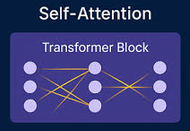
\includegraphics[width=0.55\textwidth]{Images/temp_self_attention.png}
    \legend{Fonte: Elaborado pelo autor(2026)}
    \label{fig:selfattention}
\end{figure}

\par
Essa comparação de todos os \textit{tokens} com todos os outros é justamente o que limita o tamanho da entrada.
Para uma sequência de $n$ \textit{tokens}, a autoatenção calcula $n \times n$ pesos, e \citeonline{vaswani2017attention} indicam para ela um custo por camada de $O(n^2 \cdot d)$, em que $d$ é a dimensão das representações.
Como essa matriz de pesos também precisa ser mantida em memória, o consumo de memória da atenção cresce igualmente de forma quadrática com o tamanho da sequência \cite{dao2022flashattention}: dobrar o tamanho da entrada quadruplica esse custo.
Como consequência, a submissão integral de bases de código de projetos em larga escala, como o \textit{kernel} do Linux, provoca uma explosão nos requisitos de processamento \cite{tunstall2022natural}.
\par 
Estudos empíricos confirmam que essa abordagem pode consumir dezenas de milhões de \textit{tokens} e exigir dias de processamento contínuo, criando uma limitação crítica para a escalabilidade das ferramentas \cite{hou2025generation}.
Essa sobrecarga de contexto exacerba o risco de alucinações da inteligência artificial, induzindo o modelo a gerar inferências estruturalmente plausíveis, porém tecnicamente incorretas.
\par
Para contornar as limitações da janela de contexto e o alto custo da inferência direta por um único modelo, ferramentas recentes de detecção de vulnerabilidades baseadas em LLMs têm adotado fluxos de trabalho com agentes e sistemas multi-agentes, nos quais uma tarefa complexa é decomposta entre agentes coordenados, cada um responsável por uma subtarefa localizada.
Um agente inteligente é fundamentalmente uma entidade computacional que percebe o seu ambiente e age sobre ele de alguma forma \cite{russell2020artificial}.
Em vez de submeter bases de código gigantescas a uma única instância de inteligência artificial, o processamento é descentralizado e distribuído entre múltiplos agentes.
\par
O RepoAudit, um agente baseado em LLM para auditoria de repositórios de código, por exemplo, parte justamente da constatação de que a janela de contexto limitada e o custo em tempo e em \textit{tokens} impedem que um LLM audite um repositório inteiro de uma só vez; em vez disso, seu agente explora a base de código sob demanda, função por função, e submete os resultados a um módulo validador para reduzir alucinações \cite{guo2025repoaudit}.
\par
Em um ambiente cooperativo, a comunicação e a divisão de tarefas entre os agentes emergem como comportamentos racionais essenciais para a resolução de problemas complexos \cite{russell2020artificial}.
Dessa forma, cada agente LLM assume um papel restrito e especializado, como abstração, síntese de sintaxe ou validação, colaborando de forma iterativa para reduzir a sobrecarga de \textit{tokens} e aumentar a precisão na geração do artefato final.
\par
A figura \ref{fig:motivacaocheckers} introduz motivações para a necessidade de métodos mais eficientes e, principalmente, especializados, tal que em projetos grandes, a análise estática possui dois desafios: criar regras para diversos padrões de bugs e gerenciamento de bases de códigos imensas \cite{yang2025knighter}.
Considerando esses dados, o analisador estático ideal deveria: detectar uma diversidade de falhas, incluindo \textit{corner-cases} e semânticas específicas de sistemas, e eficientemente processar milhões de linhas de código.
Porém, dos métodos existentes, geralmente sacrificam um desses objetivos \cite{yang2025knighter}.
\par
Uma proposta nessa direção é o KNighter \cite{yang2025knighter}, um sistema que usa LLMs para gerar automaticamente verificadores (\textit{checkers}) para o \textit{Clang Static Analyzer} (CSA), analisador estático de código C.
Em vez de pedir ao LLM que leia o código inteiro em busca de falhas, o KNighter fornece a ele um \textit{commit} que corrigiu um \textit{bug} real.
A partir dessa correção, o LLM descreve o padrão do \textit{bug} e escreve um verificador especializado nesse padrão, que só é aceito se apontar o código anterior à correção como defeituoso e o código corrigido como correto.
A varredura da base de código é então feita pelo próprio CSA, e não pelo LLM, o que contorna os limites da janela de contexto e o custo de analisar projetos com milhões de linhas, como o \textit{kernel} do Linux \cite{yang2025knighter}.
Assim como o RepoAudit, o KNighter também recorre a agentes auxiliares: um deles corrige erros de sintaxe nos verificadores gerados, e outro faz a triagem dos alarmes que esses verificadores produzem, descartando os falsos \cite{yang2025knighter}.
O funcionamento do KNighter é detalhado na Seção~\ref{sec:knighter}.
\par
Uma alternativa ao uso de analisadores construídos do zero são as ferramentas de análise estática baseadas em regras, como o SemGrep.
O SemGrep é uma ferramenta de código aberto na qual o usuário descreve, em arquivos no formato YAML, regras cujos padrões imitam a própria sintaxe da linguagem analisada, como ilustra a Figura \ref{fig:semgrep} \cite{hou2025generation}.

\begin{figure}[h]
    \centering
    \caption{Exemplo de regra criada para detectar uma senha embutida no argumento da função em Python.}
    \includegraphics[width=0.80\textwidth]{Images/Semgrep.png}
    \legend{Fonte: Adaptado para português com finalidade de melhorar compreensão \cite{hou2025generation}.}
    \label{fig:semgrep}
\end{figure}

\par
Ferramentas de análise estática costumam varrer o código com uma série de regras, chamada de conjunto de regras (\textit{ruleset}); uma ferramenta para C++, por exemplo, pode ter um \textit{ruleset} com verificações de vazamento de memória, de acesso fora dos limites de um vetor e de arquivos abertos e não fechados \cite{hou2025generation}.
\par
O SemGrep disponibiliza um \textit{ruleset} oficial, que \citeonline{hou2025generation} usam como referência para avaliar as regras geradas por LLMs; neste trabalho, é a esse conjunto que se refere a expressão \textit{ruleset} tradicional.
Por dispensar a construção de um analisador específico para cada tipo de falha, \citeonline{hou2025generation} utilizam o SemGrep como base para as regras que geram por meio de LLMs, abordagem também adotada neste trabalho.
Seu funcionamento é detalhado na Seção \ref{sec:analiseestaticaregras}.

\section{Formulação do problema}
\label{sec:problema}
\par
Como discutido na Seção \ref{sec:contexto}, a análise estática em projetos de larga escala precisa conciliar dois objetivos: detectar uma diversidade de falhas, incluindo \textit{corner-cases}, e processar bases de código com milhões de linhas.
Submeter o código diretamente a um LLM poderia ampliar a abrangência da detecção, mas esbarra nos limites da janela de contexto e no custo de inferência.
Diante disso, este trabalho formula a seguinte pergunta de pesquisa:

\begin{quote}
\textit{Um \textit{framework} multi-agente baseado em LLMs é capaz de sintetizar regras para o SemGrep que detectem vulnerabilidades em código C com \textit{recall} e precisão estatisticamente superiores aos do \textit{ruleset} tradicional da ferramenta?}
\end{quote}

\par
O escopo restringe-se à linguagem C, a cinco categorias de CWE (Seção \ref{sec:cwes}) e ao SemGrep como motor de execução das regras.
Não fazem parte do escopo a comparação com ferramentas de análise estática proprietárias nem a aplicação a outras linguagens de programação.
A pergunta é desdobrada nos objetivos específicos (Seção \ref{sec:objespecifico}) e na hipótese (Seção \ref{sec:hipotese}), e os resultados obtidos são discutidos no Capítulo \ref{cap:desenvolvimento}.

\section{Objetivos e hipótese}
\label{sec:objetivos}
\par
Os objetivos desta pesquisa estruturam-se em duas frentes: o objetivo geral, focado em solucionar o problema central do estudo, e os objetivos específicos, representam os subprodutos ou detalhamentos lógicos gerados para alcançar esse propósito maior.

\subsection{Objetivo geral}
\label{sec:objgeral}
\par
O objetivo geral deste trabalho é demonstrar que um \textit{framework} de síntese automatizada de regras, baseando-se em Modelos de Linguagem de Larga Escala e integrado à ferramenta SemGrep, apresenta precisão e \textit{recall} estatisticamente superiores às abordagens estáticas tradicionais na detecção de vulnerabilidades críticas em linguagem C.
Busca-se demonstrar que este modelo supera abordagens estáticas tradicionais na identificação precisa de, no mínimo, cinco categorias de vulnerabilidades de software, em inglês \textit{Common Weakness Enumeration} (CWE).
\par
Ao final da execução experimental (Capítulo \ref{cap:desenvolvimento}), este objetivo foi apenas parcialmente alcançado.
Conforme detalhado nas Seções \ref{sec:resultadoscwe416} e \ref{sec:tentativassemsucesso}, apenas uma das cinco categorias de CWE originalmente previstas (CWE-416) obteve alguma regra efetivamente aprovada pelo critério de validação definido, e de forma instável entre as sementes de particionamento avaliadas; nas demais quatro categorias (CWE-401, CWE-415, CWE-457 e CWE-476), nenhuma configuração testada atingiu os critérios mínimos de aprovação.
\par
Como os critérios de sucesso de um objetivo de pesquisa devem ser definidos antes da execução, e não ajustados depois para se adequar ao resultado obtido \cite{Wazlawick2020}, o objetivo geral foi mantido em sua forma original, e a divergência entre o planejado e o alcançado é retomada no Capítulo \ref{cap:conclusao}.

\subsection{Objetivos específicos}
\label{sec:objespecifico}
\par
Sobre os objetivos específicos, temos:

\begin{enumerate}
  \item Determinar os limites de detecção semântica (\textit{corner-cases}) que podem ser superados pela abordagem gerativa de LLMs em relação aos conjuntos de regras predefinidas (\textit{ruleset}) estáticos.
  \item Avaliar o ganho quantitativo de desempenho (\textit{Recall}, Precisão e F1-Score) de regras sintetizadas dinamicamente frente aos analisadores tradicionais do estado da arte.
  \item Determinar a viabilidade técnica e a escalabilidade de inferência da arquitetura proposta utilizando modelos de linguagem de menor escala (com contagem reduzida de parâmetros), visando garantir a viabilidade técnica da execução do \textit{framework} em infraestruturas locais com restrições de custo e \textit{hardware}.
\end{enumerate}

\par
Avaliando-se retrospectivamente cada objetivo específico à luz dos resultados do Capítulo \ref{cap:desenvolvimento}: o primeiro objetivo foi efetivamente alcançado, uma vez que o próprio processo experimental revelou um limite de detecção semântica claro e documentado para o CWE-457 (Seção \ref{sec:resultadoscwe457}), no qual a limitação não está no modelo gerador, mas no próprio motor de análise de fluxo de contaminação do SemGrep \textit{Open Source}.
\par
O segundo objetivo foi \textbf{parcialmente alcançado}: identificou-se, no registro público e gratuito do SemGrep, regras diretamente aplicáveis a duas das cinco categorias avaliadas -- \texttt{c.lang.security.function-use-after-free}, para o CWE-416, e \texttt{c.lang.security.double-free}, para o CWE-415 --, que foram executadas sobre o mesmo subconjunto rotulado do Juliet Test Suite e comparadas, em \textit{Recall}, precisão e F1-Score, com a melhor configuração sintetizada para cada CWE (Seção \ref{sec:comparacaotradicional}).
\par
A regra tradicional obteve \textit{recall} de 17,4\% (F1 de 0,276) para o CWE-416 e de 28,7\% (F1 de 0,364) para o CWE-415, contra \textit{recall} de 89,2\% a 100\% (F1 de 0,72 a 0,91) e de 43,3\% a 76,3\% (F1 de 0,50 a 0,63), respectivamente, obtidos pelas regras sintetizadas neste trabalho -- superioridade observada em todas as sementes avaliadas, sem exceção, para ambos os CWEs.
\par
Em termos práticos, \textit{recall} mede a proporção dos casos efetivamente vulneráveis do subconjunto avaliado que a regra consegue detectar -- não quantos alertas a regra emite, mas quantos dos casos que \textit{realmente contêm} a vulnerabilidade ela de fato sinaliza; cada caso vulnerável não detectado é um falso negativo, silenciosamente ignorado.
\par
Para o CWE-416, a regra tradicional (17,4\%) deixa de detectar cerca de cinco em cada seis ocorrências reais de uso após liberação presentes no subconjunto rotulado do Juliet Test Suite; a faixa de 89,2\% a 100\% obtida pela regra sintetizada neste trabalho significa que, em cada uma das cinco sementes de particionamento avaliadas (Seção \ref{sec:licaometodologica}), ao menos nove em cada dez casos vulneráveis de teste -- nunca vistos durante a geração da regra -- foram corretamente detectados, chegando à totalidade deles em algumas sementes.
\par
Para o CWE-415, a regra tradicional (28,7\%) deixa de detectar pouco mais de sete em cada dez ocorrências reais de liberação dupla; a faixa de 43,3\% a 76,3\% da regra sintetizada significa que, a depender da semente de particionamento, entre pouco menos da metade e pouco mais de três quartos dos casos vulneráveis de teste foram corretamente detectados -- uma variação mais ampla entre sementes do que a observada no CWE-416, consistente com a maior instabilidade já documentada para este CWE (Seção \ref{sec:licaometodologica}), mas ainda assim superior à regra tradicional em todas as cinco sementes, sem exceção.
\par
Em ambos os casos, o ganho de \textit{recall} não é absoluto: a Tabela \ref{tab:comparacaotradicional} mostra que, em algumas sementes, a precisão da regra sintetizada fica abaixo da precisão da regra tradicional, de modo que o ganho líquido medido pelo F1-Score -- que pondera \textit{recall} e precisão em uma única métrica --, discutido na Seção \ref{sec:comparacaotradicional}, é o indicador mais completo da comparação.
\par
Para as demais três categorias (CWE-401, CWE-457 e CWE-476), nenhuma regra do registro gratuito do SemGrep mostrou-se relevante ao padrão de vulnerabilidade avaliado, de modo que a comparação quantitativa permanece indisponível para esses casos dentro do escopo gratuito investigado, lacuna ainda reconhecida como limitação no Capítulo \ref{cap:conclusao}.
\par
O terceiro objetivo foi alcançado: a comparação entre as combinações de modelos (Seção \ref{sec:combosmodelos}) demonstrou empiricamente que modelos de menor escala (combinação C, 4 bilhões de parâmetros) são tecnicamente viáveis para a execução completa do \textit{framework} em infraestrutura local, ainda que com desempenho inferior ao de modelos maiores (combinação D) em mecanismos de correção mais refinados, como o \texttt{field\_correct} (Seção \ref{sec:resultadosfieldcorrect}).

\subsection{Hipótese ou critério de validação}
\label{sec:hipotese}
\par
A hipótese desta pesquisa é a de que a geração automatizada de regras por meio de um \textit{framework} multi-agente baseado em LLMs, integrado ao motor do SemGrep, produzirá taxas de detecção (\textit{Recall} e \textit{F1-Score}) de vulnerabilidades (CWEs) em C estatisticamente superiores e com maior identificação de \textit{corner-cases} quando comparada aos conjuntos de regras predefinidas dos analisadores estáticos tradicionais (como por exemplo \textit{ruleset} tradicional do SemGrep).
\par
Considerando os critérios de avaliação de hipóteses em pesquisa de Ciência da Computação \cite{Wazlawick2020}, esta hipótese é considerada \textbf{parcialmente confirmada}, com evidência mais direta do que a disponível na primeira redação deste capítulo.
A superioridade estatística generalizada para as cinco categorias de CWE originalmente previstas não se sustenta diante dos dados coletados (Capítulo \ref{cap:desenvolvimento}): apenas CWE-416 e CWE-415 permitiram uma comparação quantitativa direta contra um analisador tradicional, e as demais três categorias sequer foram aprovadas pelo critério de validação interno deste trabalho (Seção \ref{sec:tentativassemsucesso}); nesse sentido, a hipótese é \textbf{refutada} em sua formulação mais ampla.
\par
Por outro lado, para as duas categorias em que uma linha de base tradicional pôde ser estabelecida (Seção \ref{sec:comparacaotradicional}), a hipótese \textbf{não é refutada}: a melhor configuração sintetizada para o CWE-416 atingiu \textit{recall} de 89,2\% a 100\% e F1-Score de 0,72 a 0,91, contra 17,4\% e 0,276 da regra tradicional equivalente do registro público do SemGrep; para o CWE-415, a melhor configuração atingiu \textit{recall} de 43,3\% a 76,3\% e F1-Score de 0,50 a 0,63, contra 28,7\% e 0,364 da regra tradicional -- superando-a em \textit{recall} nas cinco sementes avaliadas, sem exceção, em ambos os CWEs.
\par
A hipótese é, portanto, refutada em sua formulação ampla (generalização irrestrita entre categorias de CWE) e sustentada por evidência quantitativa direta nos dois casos em que uma linha de base tradicional pôde ser estabelecida, conclusão discutida com maior profundidade na Seção \ref{sec:comparacaotradicional} e retomada no Capítulo \ref{cap:conclusao}.

% ---------------------------------------------------------------
\section{Justificativa}
\label{sec:justificativa}
\par
A literatura recente demonstra avanços significativos na aplicação de Modelos de Linguagem de Larga Escala, em inglês \textit{Large Language Models} (LLM), para a análise estática, comprovando a viabilidade de sintetizar verificadores automatizados de código \cite{hou2025generation, yang2025knighter}.
Trabalhos recentes atestam que a integração de LLMs com ferramentas ágeis e baseadas em regras, como o SemGrep, supera as abordagens tradicionais de lógica rígida, permitindo uma maior flexibilidade e abrangência na identificação de vulnerabilidades \cite{hou2025generation, yang2025knighter}.
\par
Contudo, apesar das evoluções trazidas pelo estudo pioneiro de \citeonline{yang2025knighter}, estudos publicados em 2025 e 2026 revelam que métodos baseados em LLMs ainda exibem uma cobertura limitada, frequentemente falhando em lidar com variações semânticas complexas e \textit{corner-cases} \cite{hou2025generation, yang2025knighter}.
Porém estudos concluíram que métodos de análise estática baseado em LLMs identificam mais vulnerabilidades únicas do que métodos tradicionais \cite{yang2025knighter, hou2025generation}.
\par
Portanto, este trabalho justifica-se pela necessidade de preencher a atual lacuna de eficácia e escalabilidade na detecção de vulnerabilidades.
O desenvolvimento de um \textit{framework} iterativo, focado na geração automatizada de regras para o motor do SemGrep, é motivado por dois problemas concretos.
\par
O primeiro é a dependência de engenharia manual: escrever regras de detecção exige conhecimento especializado, a ponto de menos de 5\% das lógicas de detecção utilizadas na indústria serem criadas por usuários comuns \cite{hou2025generation}.
\par
O segundo é o custo da inferência direta por IAs: submeter projetos inteiros a um LLM pode consumir dezenas de milhões de \textit{tokens} e exigir dias de processamento contínuo, o mesmo limite de escalabilidade já discutido na Seção \ref{sec:contexto} \cite{hou2025generation}, o que inviabiliza o seu uso contínuo.
Gerar as regras uma única vez e reutilizá-las no SemGrep, cuja execução não depende de LLMs, ataca os dois problemas simultaneamente.
\par
Ao propor um sistema especializado nas vulnerabilidades críticas (CWEs) da linguagem C, essa pesquisa visa demonstrar que é possível identificar padrões semânticos e \textit{corner-cases} com maior precisão e viabilidade técnica do que os analisadores estáticos tradicionais ou métodos generalistas baseados exclusivamente em LLMs.

% ===============================================================
% CAPÍTULO 2 - REVISÃO BIBLIOGRÁFICA / TRABALHOS RELACIONADOS
% ===============================================================
\chapter{Revisão Bibliográfica / Trabalhos Relacionados}
\label{cap:revisao}
\par
Este capítulo tem como finalidade estabelecer o embasamento teórico e tecnológico que sustenta a pesquisa proposta.
Inicialmente, descreve-se a metodologia utilizada para a seleção dos trabalhos consultados. Na sequência, o referencial teórico explora os paradigmas da análise estática assistida por inteligência artificial, as limitações da análise dinâmica e os desafios inerentes à análise estática tradicional. 
\par
Os fundamentos técnicos são apresentados com ênfase em Modelos de Linguagem de Grande Escala (LLMs), Processamento de Linguagem Natural e os princípios de Análise Estática. 
Por fim, conduz-se uma revisão dos trabalhos correlatos, identificando as lacunas que esta pesquisa busca preencher.

% ---------------------------------------------------------------
\section{Metodologia da pesquisa bibliográfica}
\label{sec:metodologia_pesquisa_bib}
\par
A pesquisa bibliográfica foi conduzida de forma sistemática para identificar trabalhos científicos relevantes sobre a utilização de LLMs no suporte à análise estática. 
As buscas foram centralizadas no motor Google Acadêmico (\textit{Google Scholar}), devido à sua ampla indexação, com foco principal em bases de dados consolidadas na área da Computação, como arXiv, IEEE Xplore e ACM Digital Library.
\par
% "static analysis" ("LLM" OR "large language model" OR "GPT") ("C" OR "C++" OR "Linux kernel") ("pointer" OR "undefined" OR "memory" OR "value-flow") ("SemGrep" OR "semgrep")
Para as buscas, foram definidas palavras-chave em inglês, tais como: \textit{``static analysis''}, \textit{``LLM''}, \textit{``large language model''}, \textit{``GPT''}, \textit{``C''}, \textit{``C++''}, \textit{``rule generation''}, \textit{``Linux kernel''}, \textit{``pointer''}, \textit{``undefined''}, \textit{``memory''}, \textit{``value-flow''} e \textit{``SemGrep''}. 
Estes termos foram combinados por meio de operadores booleanos (\textit{AND}, \textit{OR}) para refinar os resultados, culminando na \textit{string} de busca apresentada na Figura \ref{fig:query}:

\begin{figure}[h]
    \centering
    \caption{\textit{Query} utilizada durante a pesquisa de materiais.}
    \includegraphics[width=0.98\textwidth]{Images/Query.png}
    \legend{Fonte: Elaborado pelo autor (2026)}
    \label{fig:query}
\end{figure}

\par
Como critérios de inclusão, estabeleceram-se: (a) trabalhos publicados entre 2021 e 2026, de forma a capturar o estado da arte; (b) disponibilidade nos idiomas inglês ou português; e (c) relação direta com o tema, priorizando artigos que contivessem implementações ou experimentos aplicados à utilização de LLMs para geração de regras para a linguagem C.
\par
Em contrapartida, os critérios de exclusão adotados foram: (a) trabalhos publicados antes de 2021, com exceção de referências clássicas ou seminais indispensáveis para a teoria; (b) artigos sem alinhamento direto com análise estática ou geração de regras de código; e (c) duplicidades de publicações entre as bases de dados consultadas.
\par
O processo de seleção ocorreu em duas etapas. 
Na primeira fase (triagem), a aplicação da \textit{string} de busca retornou 4.770 resultados, dos quais foram selecionados 47 artigos potencialmente relevantes após a leitura prévia de títulos e resumos. 
Na segunda fase (afunilamento), os trabalhos restantes passaram por uma leitura criteriosa da introdução e do escopo, sendo classificados em uma escala de relevância de 0 a 10 em relação aos objetivos desta pesquisa.

\begin{figure}[h]
    \centering
    \caption{Funil de pesquisa.}
    \includegraphics[width=0.75\textwidth]{Images/Funil.png}
    \legend{Fonte: Elaborado pelo autor (2026)}
    \label{fig:funil}
\end{figure}

\par
A avaliação de 0 a 10 foi feita a partir de seu resumo, palavras-chave, tecnologia aplicada. Caso o trabalho possua similaridades com outros artigos bem avaliados é considerado como suporte ou alta relevância. 
Esse processo de filtragem resultou em 6 artigos classificados com notas entre 9 e 10 (alta relevância), além de 9 artigos categorizados como material de suporte, totalizando 15 trabalhos contemporâneos para compor a fundamentação teórica. 
Adicionalmente, foram incorporados 5 trabalhos seminais anteriores a 2021, essenciais para a consolidação dos conceitos clássicos abordados neste estudo.

% ---------------------------------------------------------------
% ---------------------------------------------------------------
\section{Fundamentos teóricos}
\label{cap:referencial}
\par
O referencial teórico apresenta os conceitos fundamentais que sustentam o desenvolvimento deste projeto. 
Propõe-se um contraponto analítico entre os métodos da análise estática tradicional e as novas abordagens voltadas à automatização da geração de regras.
\par 
A estruturação dos tópicos foi concebida para apresentar gradativamente as tecnologias envolvidas, destacando o papel das LLMs e sua relevância para a modernização das ferramentas de verificação de código na atualidade.

\subsection{Análise Estática Tradicional}
\label{sec:analisetradicional}
\par
Verificações estáticas, segundo \citeonline{aho2007compilers}, são checagens de consistência realizadas durante o processo de compilação, sendo possível capturar erros de programação cedo, antes da sua execução. 
\par
Incluindo dois tipos de análises: 
\textbf{(i) Verificação Sintática}, envolve a aplicação de restrições que não são aplicadas apenas pelas gramáticas, como um identificador ser declarado apenas uma vez dentro do escopo \cite{aho2007compilers}.
\textbf{(ii) Verificação de Tipos}, assegura que as regras de tipagem da respectiva linguagem sejam seguidas, checando se os operadores ou funções estão sendo aplicados ao número ou tipo correto de operando.
Se a conversão de tipos é necessária, o verificador pode inserir o operador correto na árvore de sintaxe para a conversão \cite{aho2007compilers}.
\par
Não é importante somente para otimização de código, as mesmas técnicas podem ser usadas para analisar \textit{software} já existentes para diversos padrões comuns de erros de programação \cite{aho2007compilers}.
PREfix e Metal são duas ferramentas mencionadas por \citeonline{aho2007compilers} utilizam análise estática interprocedural, rastreando o fluxo de informações em um programa inteiro, para encontrar erros de programação estaticamente em grandes bases de código.
Estas ferramentas são capazes de rastrear o caminho de entradas fornecidas pelos usuários enquanto essas \textit{strings} são copiadas ou combinadas ao longo de vários procedimentos, acompanhando as entradas é possível prevenir contra \textit{SQL Injection} e \textit{Buffer Overflows} \cite{aho2007compilers}.

\subsubsection{Árvore Sintática Abstrata}
\label{sec:ast}
\par
Durante o processo de análise sintática, é comum a geração de uma árvore de análise (\textit{Parse Tree}), também conhecida como árvore de sintaxe concreta, onde os nós internos representam os símbolos não-terminais definidos pela gramática da linguagem \cite{aho2007compilers}.
Contudo, para as fases subsequentes de compilação ou de análise estática de código, essa representação contém detalhes puramente estruturais que não afetam a semântica do programa \cite{aho2007compilers}.
\par
A Árvore Sintática Abstrata, do inglês \textit{Abstract Syntax Tree} (AST), surge como uma representação intermediária otimizada.
Em uma AST, cada nó interno representa um operador ou um constructo de programação, enquanto nós filhos representam os operandos ou os componentes semânticos daquele constructo \cite{aho2007compilers}.
Nós auxiliares exigidos pela gramática para contornar ambiguidades ou definir precedência (como produções única ou parênteses) são descartados, resultando em uma estrutura de dados mais limpa e focada no significado das operações \cite{aho2007compilers}.

\begin{figure}[h]
    \centering
    \caption{Árvore Sintática Abstrata para a expressão 9-5+2}
    \includegraphics[width=0.45\textwidth]{Images/AST.png}
    \legend{Fonte: \cite{aho2007compilers}}
    \label{fig:ast}
\end{figure}

\par
Tomando como exemplo, na figura \ref{fig:ast}, a expressão matemática 9 - 5 + 2, a raiz da AST representaria o operador +, tendo como filho esquerdo a subexpressão correspondente a 9 - 5 e como filho direito a constante 2.
Esse agrupamento estrutural reflete a precedência e a associatividade à esquerda dos operadores, tornando redundante a presença de nós sintáticos adicionais.
\par
Em ferramentas de análise estática voltadas para linguagens complexas como C, operar sobre a AST é essencial, pois permite que a verificação de propriedades e a busca por vulnerabilidades sejam conduzidas diretamente sobre a lógica estrutural do código, isolando a análise de variações gramaticais irrelevantes \cite{aho2007compilers}.
\par
No contexto da análise de vulnerabilidades, a AST é fundamental para identificar padrões estruturais perigosos.
Ao invés de realizar buscas textuais limitadas, os analisadores percorrem a árvore em busca de composições específicas de nós.
\par
Por exemplo, para detectar um risco de desreferenciação de ponteiro nulo (\textit{Null Pointer Dereference}), uma regra de análise pode inspecionar a AST em busca de um nó que represente uma chamada de alocação de memória, como a função \texttt{devm\_kzalloc}, verificando se não existe um nó condicional adjacente encarregado de checar o valor de retorno antes de sua utilização.

\subsubsection{Grafos de Fluxo de Controle}
\label{sec:gfc}
\par
Complementar à Árvore Sintática Abstrata (AST), utilizam-se os grafos de fluxo de controle, do inglês \textit{Control Flow Graphs} (CFG).
Enquanto a AST foca em representar hierarquicamente a sintaxe estrutural do código, o CFG é um grafo direcionado construído para modelar os possíveis caminhos de execução do programa, sendo a base essencial para análises sensíveis ao fluxo (\textit{flow-sensitive}) \cite{aho2007compilers}.
\par
Representação em grafo de código intermediário é muito útil para a geração de código \cite{aho2007compilers}.
De acordo com \citeonline{aho2007compilers}, essa representação é construída em dois passos, primeiro, é particionado o código intermediário em blocos básicos (\textit{basic blocks}), que atuam como os nós do grafo.
\par
Um bloco básico é uma sequência máxima de instruções consecutivas de três endereços onde o fluxo de controle entra obrigatoriamente pela primeira instrução, sem saltos para o interior dele, e sai apenas pela última, sem interrupções ou ramificações em seu interior \cite{aho2007compilers}.
As arestas relacionadas do grafo indicam as transições de controle (\textit{control flow}) permitidas no programa, representando que a execução pode fluir do final de um bloco básico específico para o início de outro \cite{aho2007compilers}.
\par
Na construção de um CFG, as instruções de desvio (\textit{jumps}) endereçadas a linhas ou rótulos específicos são substituídas por referências diretas aos blocos básicos correspondentes.
Essa abstração é fundamental na construção de compiladores, pois permite que otimizações subsequentes alterem livremente o conteúdo interno dos blocos sem invalidar os alvos dos desvios de controle \cite{aho2007compilers}.
Caso não houvesse essa otimização, seria necessário corrigir os alvos toda vez que uma instrução fosse alterada.
\par
CFGs podem ser representados na programação por qualquer estrutura de dados tradicional para grafos. 
Quanto ao conteúdo interno dos nós (blocos básicos), \citeonline{aho2007compilers} afirma que eles podem ser representados por um ponteiro para a primeira instrução e uma contagem de instruções.
No entanto, como as otimizações alteram frequentemente a quantidade de instruções, costuma ser mais eficiente representar o conteúdo de cada bloco básico, ou nó, como uma lista encadeada (\textit{linked list}) de instruções \cite{aho2007compilers}.

\subsubsection{Análise de Fluxo de Dados}
\label{sec:analisefluxo}
\par
A Análise de Fluxo de Dados, em inglês \textit{Data Flow Analysis} (DFA), é definida como um conjunto de técnicas que derivam informações sobre o fluxo de dados ao longo dos possíveis caminhos de execução de um programa \cite{aho2007compilers}.
\par
Tradicionalmente fundamentais para as otimizações globais em compiladores, essas técnicas permitem determinar, por exemplo, se duas expressões avaliam para o mesmo valor em todos os caminhos possíveis ou se o resultado de uma atribuição nunca é utilizado (código morto) \cite{aho2007compilers}.
\par
A execução de um programa é modelada como uma série de transformações do estado do programa, onde o estado consiste nos valores de todas as variáveis do programa em um dado momento \cite{aho2007compilers}.
Cada instrução executada transforma um estado de entrada em um novo estado de saída.
\par
No entanto, \citeonline{aho2007compilers} afirma que é impossível acompanhar todos os estados exatos devido ao número ilimitado de caminhos de execução.
Por esse motivo, a DFA opera através de abstrações, ignorando detalhes irrelevantes e guardando apenas as características essenciais para o objetivo da otimização \cite{aho2007compilers}.
\par
É associado a cada ponto do programa um valor de fluxo de dados (que representa a abstrações dos estados possíveis) pertencente a um ``domínio'' \cite{aho2007compilers}.
O problema de DFAs consiste em encontrar uma solução para dois conjuntos de restrições principais:
\par
\textbf{Funções de transferência} (\textit{Transfer Functions}), são restrições baseadas na semântica de cada instrução, pegando o valor do fluxo de dados antes da instrução e geram um novo valor de saída \cite{aho2007compilers}.
O fluxo pode acontecer ``para frente'' (\textit{forward}), onde a entrada molda a saída, ou ``para trás'' (\textit{backward}), onde a direção desse fluxo é invertida.
\par
\textbf{Restrições de Fluxo de Controle} (\textit{Control-Flow Constraints}), definem como a informação transita de um bloco básico para outro dentro do CFG. 
Essencialmente, o valor do fluxo de dados que entra em uma instrução é matematicamente determinado pela combinação dos valores que saem das instruções ou blocos predecessores \cite{aho2007compilers}.
\par
No contexto da segurança de \textit{software} e da detecção de falhas abordadas neste trabalho, a abstração fornecida pela DFA é o motor principal que permite analisadores estáticos avançados identificarem vulnerabilidades complexas.
É através do rastreamento do estado das variáveis pelos caminhos de controle que se torna viável detectar comportamentos críticos em linguagens como C, como \textit{Null Pointer Dereference} (CWE-476) ou uso de variáveis não inicializadas (CWE-457).

\subsubsection{Sensibilidade de Fluxo}
\label{sec:sensifluxo}
\par
A precisão de uma análise estática depende fortemente de sua sensibilidade ao fluxo de controle.
Segundo \citeonline{aho2007compilers}, as abordagens de análise (como a análise de apontamento de ponteiros) podem ser categorizadas em dois tipos principais:
\par
\textbf{Análise Sensível ao Fluxo}, em inglês \textit{Flow-Sensitive Analysis} (FSA), essa abordagem acompanha o fluxo de controle do programa e computa o estado exato (por exemplo, para onde cada variável pode apontar) após a execução de cada instrução individual \citeonline{aho2007compilers}.
Isso significa que a análise avalia as restrições e funções de transferência passo a passo; ela não apenas considera novas informações e relações que um comando gera (\textit{generate}), mas também contabiliza as informações anteriores que o comando invalida ou mata (\textit{kills}).
\par
\textbf{Análise Insensível ao Fluxo}, em inglês \textit{Flow-Insensitive Analysis} (FIA), em contrapartida, essa abordagem ignora o fluxo de controle, assumindo essencialmente que cada instrução do programa pode ser executada em qualquer ordem \cite{aho2007compilers}.
A FIA computa apenas um mapa global indicando para onde cada variável possivelmente apontar em qualquer momento da execução do programa.
Em uma análise insensível ao fluxo, uma atribuição nunca invalida (\textit{kill}) relações de apontamento; ela apenas gera novas relações. Ou seja, se uma variável puder apontar para dois objetos diferentes após a avaliação de duas instruções distintas, o sistema apenas registra e acumula a informação global de que ela aponta para ambos \cite{aho2007compilers}.
\par
\citeonline{aho2007compilers} explicam que a falta de sensibilidade ao fluxo enfraquece consideravelmente a precisão dos resultados da análise, uma vez que produz superaproximações do estado real do programa. 
No entanto, essa abstração tem o benefício direto de reduzir drasticamente o tamanho da representação dos resultados e fazer com que o algoritmo termine de forma mais rápida, o que é frequentemente necessário ao analisar bases de código em larga escala.

\subsubsection{Limitações da Análise Estática}
\label{sec:limitacoesanalise}
\par
\citeonline{aho2007compilers} explicam que o problema de encontrar todos os erros de um programa é indecidível.
Uma ferramenta de análise de fluxo de dados pode até ser projetada para alertar programadores sobre todas as possíveis partes do código com uma categoria específica de erros, porém se a maioria desses avisos forem falsos alarmes, os usuários não vão utilizar a ferramenta.
\par
Por conta dessa complexidade, \citeonline{aho2007compilers} afirmam que os detectores práticos de erros frequentemente não são perfeitos (à prova de falhas ou \textit{sound}) nem completos (\textit{complete}).
As abordagens tradicionais de detecção de vulnerabilidades estática geralmente codificam o conhecimento especializado como regras projetadas manualmente, com padrões e modelos de fluxo de dados, sua dependência de padrões predefinidos limita inerentemente a generalização e a cobertura para tipos de vulnerabilidades previamente não vistos ou em evolução.
\par
Isso significa que a análise estática pode não encontrar todos os erros no programa, e nem todos os erros relatados têm a garantia de serem erros reais, e se as ferramentas relatassem todos os erros potenciais, o volume de falsos positivos tornaria as ferramentas inutilizáveis \cite{aho2007compilers}.

\subsubsection{Análise estática baseada em regras}
\label{sec:analiseestaticaregras}
\par
Em anos recentes, ferramentas de análise estática baseada em regras foram introduzidas.
Complementando as ferramentas tradicionais, ao identificar previamente problemas durante o desenvolvimento pré-produção, reduzem significamente o custo e complexidade de \textit{debugging} e manutenção \cite{jiang2025factaligned}.
Dos componentes mais utilizados, um dos mais relevantes são SemGrep e CodeQL \cite{jiang2025factaligned, hou2025generation}.
\par 
Formalmente, SemGrep é uma ferramenta de análise estática que suporta estruturas complexas e verificações básicas de fluxo de dados no código, permitindo inspeções sem execução para identificar vulnerabilidades de segurança, qualidade de código e violações a conformidade \cite{hou2025generation}.
\par
Sua gramática baseada em YAML mimetiza a sintaxe da linguagem alvo, reduzindo sua curva de aprendizado ao contrário de seu concorrente CodeQL \cite{hou2025generation}, que possui sua própria gramática lógica, tratando o código como um banco de dados relacional, sendo possível realizar análises profundas porém custosa em tempo de aprendizado.
\par
SemGrep converte código em uma árvore de sintaxe abstrata universal (UAST), aplicando um \textit{pattern-matching} uniforme em mais de 30 linguagens \cite{hou2025generation}.
Por ser um projeto mantido ativamente e contar com uma plataforma pública na qual a comunidade compartilha regras prontas, o SemGrep facilita a adaptação de regras existentes e o desenvolvimento colaborativo.

\begin{figure}[h]
    \centering
    \caption{Exemplo de regra simplificada para detecção de falhas OSCI em Java.}
    \includegraphics[width=0.95\textwidth]{Images/Semgrep-java.png}
    \legend{Fonte: Adaptado de \cite{jiang2025factaligned}.}
    \label{fig:semgrepjava}
\end{figure}

\par
\citeonline{jiang2025factaligned} utilizam a regra da Figura \ref{fig:semgrepjava} para ilustrar a utilidade prática do SemGrep: ela identifica, em código Java, uma falha de injeção de comandos no sistema operacional, do inglês \textit{Operating System Command Injection} (OSCI).
\par
Para que a busca seja flexível e rastrear fluxo de dados, o SemGrep utiliza dois recursos fundamentais: 
\par
(i) \textbf{Metavariáveis} (ex.: \textit{\$USER\_DATA}, \textit{\$X}), a partir de um cifrão e nome da variável em letras maiúsculas.
Essas variáveis são atribuídas quando SemGrep identifica um padrão que se encaixa, sendo ``salvo'' o valor na metavariável, consequentemente, se a metavariável é reutilizada na mesma regra, o SemGrep exigirá que o valor capturado seja exatamente o mesmo, o que permite \textit{Data Flow}.
\par
(ii) \textbf{Ellipsis/Curinga} (...), representando qualquer sequência de coisas.
Assim independente da quantidade de argumentos em uma função, número de linhas de código entre duas instruções, é possível omitir detalhes não importantes com (...), tornando SemGrep uma ferramenta abstraída.
\par
Os predicados são as afirmações que procuram o código.
\textit{Tags} como \textit{pattern} ou \textit{pattern-inside} são predicados, com \textit{\textbf{pattern}} sendo uma afirmação exata, como na linha 5, e \textit{\textbf{pattern-inside}} define o contexto, não apontando a vulnerabilidade exata, mas exige que qualquer correspondência subsequente aconteça dentro da estrutura dele, como na linha 2.
\par
A partir destes predicados, é possível combinar operações lógicas (\textit{AND}, \textit{OR}, \textit{NOT}) sendo, respectivamente, \textit{patterns}, \textit{pattern-either}, \textit{pattern-not}.
\par
(i) O predicado \textit{\textbf{patterns}} representa a lógica \textit{AND} (E), para toda regra ou condição listada abaixo deste bloco devem ser verdadeiras simultaneamente.
Como na linha 1, o bloco principal exige que o código esteja dentro da função (linha 2) \textbf{E} corresponda a um dos casos de injeção (linha 4).
\par
(ii) \textbf{\textit{pattern-either}} representa a lógica \textit{OR} (OU), se o código corresponde a qualquer uma das condições aninhadas sob este predicado, a avaliação será verdadeira. Na linha 4, a regra procura um fluxo direto de \textit{\$USER\_DATA} ou um fluxo indireto por atribuição.
\par
(iii) \textbf{\textit{pattern-not}} representa a lógica \textit{NOT} (NÃO).
Não presente no exemplo, porém usado para excluir falsos positivos, anulando caso a regra bater com a condição aninhada no predicado.
\par
Com estes conhecimentos, é possível compreender como o SemGrep lida nativamente com falsos positivos.
Predicados de exclusão, como \textit{pattern-not} e \textit{pattern-not-inside}, descartam ocorrências que já estão protegidas, por exemplo, o uso de um ponteiro que foi verificado contra \texttt{NULL} logo antes, enquanto \textit{pattern-inside} restringe a busca ao contexto em que a falha de fato pode ocorrer.
Assim, cada regra pode ser refinada de forma incremental, acrescentando exclusões para os falsos positivos observados, o que é explorado pelo \textit{pipeline} proposto neste trabalho.

\subsection{Vulnerabilidades de Linguagem}
\label{sec:vulnerabilidadeslinguagem}
\par
O termo Vulnerabilidade (\textit{Vulnerability}) é definido como um conjunto de condições que permite que um invasor (atacante) viole uma política de segurança explícita ou implícita \cite{seacord2013secure, seicertc2016}.
Nem toda falha de segurança (\textit{security flaw}) leva a uma vulnerabilidade \cite{seacord2013secure}.
\par
\citeonline{seacord2013secure} explicam que para que uma falha torne um programa vulnerável a ataques, é necessário que os dados de entrada desse programa cruzem um limite de segurança (\textit{security boundary}).
Uma falha pode existir no código sem as pré-condições para ser explorada; por exemplo, se o programa apresentar um erro grave mas não possuir permissões para ser acessado localmente, ele não viola a política de segurança e não constitui uma vulnerabilidade ativa \cite{seacord2013secure}.
\par
Uma vulnerabilidade pode existir mesmo sem que haja uma falha ou defeito no código \cite{seacord2013secure}.
Como a segurança é um atributo de qualidade que muitas vezes precisa ser balanceado com outros fatores (como desempenho e usabilidade), os projetistas de \textit{software} podem decidir intencionalmente deixar um produto vulnerável a certas formas de exploração \cite{seacord2013secure}.
Isso representação uma aceitação consciente do risco pelo projetista e não um erro de programação.

\subsubsection[\textit{Common Vulnerabilities and Exposures}]{\textit{Common Vulnerabilities and Exposures}}
\label{sec:cves}
\par
A Enumeração Comum de Vulnerabilidades e Exposições, mais popularmente conhecida do inglês \textit{Common Vulnerabilities and Exposures} (CVE).
Similarmente à CWEs, CVE atua como um dicionário, com foco em identificar, definir e catalogar vulnerabilidades de segurança cibernética que foram divulgadas publicamente \cite{cveabout}.
\par 
CVE possui um único registro no seu catálogo para cada vulnerabilidade descoberta para uma versão específica de um \textit{software}.
O objetivo principal de se atribuir um CVE é permitir que profissionais de TI, ferramentas automatizadas e equipes de segurança cibernética saibam que estão se referindo exatamente ao mesmo problema \cite{cveabout}.
\par
Após a confirmação de uma vulnerabilidade, ela recebe um identificador único composto pelo ano de relato ou atribuição, seguido por um sequencial numérico.
Parceiros como \textit{National Vulnerability Database} (NVD) adicionam o registro com suas descrições, atribuindo um índice de severidade metrificado pela \textit{Common Vulnerability Scoring System} (CVSS) e sua causa raiz proveniente da CWE \cite{cveabout}.

\subsubsection{\textit{Common Weakness Enumeration}}
\label{sec:cwes}
\par
A Enumeração de Fraquezas Comuns, mais popularmente conhecida do inglês \textit{Common Weakness Enumeration} (CWE), é um dicionário formal e uma lista desenvolvida pela comunidade que cataloga fraquezas comuns de \textit{software} e \textit{hardware} \cite{mitrecwe}.
\par
Neste contexto, o termo fraqueza (\textit{weakness}) é definido como uma condição em um componente de \textit{software}, \textit{firmware}, \textit{hardware} ou serviço que, sob determinadas circunstâncias, pode contribuir para a introdução de vulnerabilidades \cite{mitrecwe}.
O projeto identifica, classifica e descreve esses problemas sob a nomenclatura de CWEs individuais (como, por exemplo, CWE-476 \textit{Null Pointer Dereference}).
\par
O propósito principal de se mapear essas fraquezas é permitir que desenvolvedores de \textit{software}, projetistas de \textit{hardware} e arquitetos de segurança as eliminem ainda na fase de desenvolvimento, antes da implantação (\textit{deployment}), o que torna a correção muito mais fácil e barata.
\par 
O conteúdo de CWEs pode ser navegado através de diferentes visões, agrupando fraquezas para domínios específicos, como visões focadas estritamente em conceitos de Desenvolvimento de \textit{Software}, organizando as falhas que surgem durante a programação), Design de \textit{Hardware} e Conceitos de Pesquisa, organizando as falhas por comportamentos \cite{mitrecwe}.
\par
O dicionário CWE fornece mapeamentos externos essenciais e atua como base para diversos outros recursos e guias de segurança fundamentais na indústria, como as listas \textbf{CWE Top 25}, \textbf{OWASP Top 10} e os \textbf{padrões de codificação segura do SEI CERT} \cite{mitrecwe, seicertc2016}.
A lista de fraquezas é atualizada de três a quatro vezes por ano para adicionar ou aprimorar informações, e o dicionário é construído, em parte, tomando como base os problemas reportados nos registros de vulnerabilidades ativas do catálogo CVE, do inglês \textit{Common Vulnerabilities and Exposures}.
\par
Para o escopo deste trabalho, serão consideradas primariamente cinco vulnerabilidades presentes na lista oficial da CWE, todas são fraquezas relacionadas a falhas de memória.
São elas:

\begin{itemize}
  \item \textbf{CWE-401}: \textit{Missing Release of Memory after Effective Lifetime}; 
  \item \textbf{CWE-415}: \textit{Double Free}; 
  \item \textbf{CWE-416}: \textit{Use After Free}; 
  \item \textbf{CWE-457}: \textit{Use of Uninitialized Variable};
  \item \textbf{CWE-476}: \textit{Null Pointer Dereference}. 
\end{itemize}

\subsubsection{CWE-401}
\label{sec:401}
\par
A CWE-401, chamada de Vazamento de Memória, do inglês \textit{Missing Release of Memory after Effective Lifetime} ou \textit{Memory Leak}, ocorre quando um programa aloca memória, mas falha em rastreá-la ou liberá-la adequadamente após ela não ser mais necessária \cite{cwe401}. 
Isso torna o bloco de memória indisponível para realocação ou reúso.
\par
De acordo com \citeonline{cwe401}, é frequentemente causada por caminhos de execução, como condições de erro, dados malformados ou sessões interrompidas abruptamente, onde o código falha em executar a rotina de limpeza.
Também surge da confusão sobre qual parte do programa é responsável por realizar o \textit{free} em linguagens de gerenciamento manual, como C.
\par
Embora normalmente resulte em problemas gerais de confiabilidade do \textit{software}, se um invasor conseguir desencadear repetidamente esse vazamento de forma intencional, ele poderá esgotar a memória do sistema \cite{cwe401}.
Consequentemente leva a uma Negação de Serviço, em inglês \textit{Denial of Service} (DoS) por consumo excessivo de resursos (CPU ou memória) ou travamentos.
\par
A melhor forma é utilizar linguagens, bibliotecas ou \textit{frameworks} que forneçam gerenciamento automático de memória (como \textit{garbage collectors}) \cite{cwe401}.
Linguagens como C, contudo, não oferecem esse gerenciamento de forma nativa.
A adoção de bibliotecas externas para suprir essa falta exige cautela do projetista, que deve ponderar o custo de desempenho (\textit{overhead}), o risco de introdução de novas vulnerabilidades pela própria biblioteca e o aumento no esforço de análise de segurança do sistema.

\subsubsection{CWE-415}
\label{sec:415}
\par
A CWE-415, chamada de Liberação Dupla, do inglês \textit{Double Free}, ocorre quando o produto chama a função de liberação (como \texttt{free()}) duas vezes no mesmo endereço de memória \cite{cwe415}.
\par
Semelhante ao vazamento de memória (\ref{sec:401}), costuma ser resultado de condições de erro não tratadas corretamente ou confusão lógica sobre a responsabilidade de limpar a memória, especialmente quando ponteiros são usados de forma global ou espalhados por centenas de linhas e múltiplos arquivos \cite{cwe415}.
\par
Chamar a função \texttt{free()} de forma dupla corrompe as estruturas de dados de gerenciamento de memória do sistema.
O programa pode travar, ou, pior, fazer com que duas chamadas futuras da função \texttt{malloc()} retornem exatamente o mesmo ponteiro \cite{cwe415}.
Se o invasor controlar os dados inseridos nessa memória ``duplamente alocada'', ele ganha uma condição conhecida como \textit{write-what-where} e pode realizar ataques de \textit{buffer overflow}, chegando a \textbf{executar código arbitrário} \cite{cwe415}.
\par
Para garantir que cada alocação seja liberada apenas uma vez, uma técnica prática é definir o ponteiro como \texttt{NULL} imediatamente após o primeiro \texttt{free}, garantindo que não possa ser liberado novamente por engano \cite{cwe415}.

\subsubsection{CWE-416}
\label{sec:416}
\par
A CWE-416, chamada de Uso Após Liberação, do inglês \textit{Use After Free} (UAF), ocorre quando o programa continua a utilizar ou referenciar um ponteiro para a memória que já foi liberada \cite{cwe416}.
Como a memória já foi devolvida, ela pode ter sido realocada e preenchida com dados novos; logo, as operações realizadas com o ponteiro original interagem acidentalmente com os dados da nova alocação \cite{cwe416}.
\par 
Frequentemente resulta de outras fraquezas primárias, como, em concorrência, condições de corrida, manipulação inadequada de erros ou apenas liberação precoce por falha lógica \cite{cwe416}.
\par 
É possível causar alteração não intencional de memória, corrompendo dados válidos, vazamento de informações confidenciais, como permissão de leitura indevida, e DoS por travamento \cite{cwe416}.
Além disso, se o invasor conseguir inserir dados maliciosos logo após o ponteiro ser liberado, é possível \textbf{executar códigos ou comandos arbitrários} assumindo o controle da execução \cite{cwe416}.
\par
Além do uso de gerenciamento automático, usar o conceito visto em CWE-415 (\ref{sec:415}), definindo os ponteiros como \texttt{NULL} imediatamente após serem liberados.
Se houver uma falha que tente reutilizar esse ponteiro depois disso, ocorrerá um travamento (Desreferenciamento de Nulo), mas isso elimina a possibilidade crítica de execução de código malicioso \cite{cwe415}.

\subsubsection{CWE-457}
\label{sec:457}
\par
A CWE-457, chamada de Uso de Variável Não Inicializada, do inglês \textit{Use of Uninitialized Variable}, ocorre quando o código usa uma variável que não recebeu um valor inicial \cite{cwe457}.
Em linguagens como C, variáveis armazenadas na pilha (\textit{stack}) não são limpas por padrão e conterão lixo de memória deixado por chamadas de funções anteriores.
\par
Segundo \citeonline{cwe457}, tipicamente ocorre por erros tipográficos no código ou porque um fluxo lógico (como \texttt{switch} ou \texttt{if/else}) falhou em cobrir todos os casos e não atribuiu valor à variável antes de ela ser utilizada.
\par
Essa fraqueza pode gerar comportamentos totalmente imprevisíveis, corromper o fluxo de controle esperado do programa ou causar DoS.
Em cenários críticos, um invasor pode influenciar os dados residuais na pilha (pré-inicializando o lixo intencionalmente) para contornar checagens de senha, burlar travas lógicas ou \textbf{executar código} \cite{cwe457}.
O problema se agrava com \textit{strings}, pois funções contam com um terminador nulo que pode não existir no lixo residual.
\par
Sempre garantir explicitamente que variáveis essenciais recebam um valor padrão aceitável no momento de declaração \cite{cwe457}.
É fortemente recomendado configurar e usar ferramentas de compilação em modos rigorosos, pelos compiladores moderrnos costumarem emitir alertas consistentes quando variáveis são lidas sem serem inicializadas \cite{cwe457}.

\subsubsection{CWE-476}
\label{sec:476}
\par
A CWE-476, chamada de Desreferenciamento de Ponteiro Nulo, do inglês \textit{Null Pointer Dereference}, ocorre quando o código tenta desreferenciar, acessar o conteúdo ou método apontado, um ponteiro sob a suposição de que ele é válido, mas seu valor real é \texttt{NULL} \cite{cwe476}.
\par
Muitas funções de busca ou resolução de rede (por exemplo: \texttt{gethostbyaddr}) retornam nulo quando falham, e os desenvolvedores se esquecem de checar o retorno (\textit{Unchecked Return Value}) antes de usar o resultado do ponteiro \cite{cwe476}.
Também pode ser consequência de variáveis não inicializadas ou concorrência em sistemas assíncronos.
\par
Segundo \citeonline{cwe476}, a consequência geralmente é o \textbf{travamento completo do processo} (DoS), sendo muito difícil que o programa se recupere para um estado seguro de funcionamento, mesmo com tratamentos de exceção.
Em raras circunstâncias, como quando \texttt{NULL} equivale ao endereço de memória literal \texttt{0x00} e o código privilegiado pode acessá-lo, um invasor pode ler/escrever na memória e \textbf{executar códigos} \cite{cwe476}.
\par
Validar e checar estritamente resultados de todas as funções, confirmando que o valor não é nulo antes de utilizá-lo. Inicializar variáveis com valores padrões também previnem essa situação \cite{cwe476}.

\subsection{Linguagem Natural}
\label{subsec:linguagemnatural}
\par
Um sistema formal amplamente utilizado para modelar a estrutura constituinte em linguagens naturais é a Gramática Livre de Contexto (\textit{Context-Free Grammar} - CFG). 
Também conhecidas como gramáticas de estrutura de frase (\textit{phrase-structure grammars}), as CFGs utilizam um formalismo que é equivalente à Forma de Backus-Naur (BNF), padrão universal para a especificação da sintaxe em computação \cite{jurafsky2026speech}.
\par
Uma CFG consiste em um conjunto de regras ou produções, onde cada uma expressa como os símbolos podem ser ordenados e agrupados, e um léxico de palavras e símbolos.
Tal estrutura define uma linguagem formal, na qual existe uma separação estrita: sentenças que podem ser derivadas pelas regras são consideradas gramaticais, enquanto as que não podem são denominadas agramaticais \cite{jurafsky2026speech}.
\par
Contudo, essa distinção rígida é uma característica das gramáticas formais e serve apenas como um modelo simplificado das linguagens naturais.
Diferente das linguagens de programação, a validade e o sentido em linguagem natural dependem intrinsecamente do contexto.
Na linguística computacional, o uso desses modelos para capturar tal complexidade é fundamentado na gramática generativa, visto que a linguagem passa a ser definida pelo conjunto de possíveis 'geradas' por suas regras gramaticais \cite{jurafsky2026speech}.

\subsubsection{Processamento de Linguagem Natural}
\label{sec:processamentoln}
\par
O Processamento de Linguagem Natural, do inglês \textit{Natural Language Processing} (NLP), tem de objetivo fundamental capacitar os sistemas computacionais a processar, armazenar, compreender e gerar a linguagem humana, permitindo que as máquinas se comuniquem com sucesso e realizem tarefas inferenciais complexas \cite{jurafsky2026speech}.
\par
Os autores pontuam que o problema da compreensão da linguagem é consideravelmente complexo, pois não se restringe apenas ao entendimento da estrutura sintática das sentenças, mas exige uma profunda compreensão da semântica, do contexto e do assunto abordado.
\par
O campo de NLP progrediu através de diferentes abordagens de resolução, a abordagem mais relevante para este trabalho é o Aprendizado Profundo (\textit{Deep Learning}).
Baseado na arquitetura \textit{Transformer}, esse paradigma mudou o foco da engenharia manual de características para a aprendizagem de representação (\textit{representation learning}), onde os modelos aprendem automaticamente vetores de significado contínuos (\textit{embeddings} contextuais) operando em vastas quantidades de texto não rotulado, mediante o pré-treinamento autossupervisionado \cite{jurafsky2026speech}.
\par
O NLP é dividido em tarefas de Compreensão de Linguagem Natural (\textit{Natural Language Understanding} - NLU), focadas em extrair significado, e Geração de Linguagem Natural (\textit{Natural Language Generation} - NLG), focadas na produção de texto coerente \cite{tunstall2022natural}.
\par
Para modelos mais utilizados de LLMs, o foco inerente desses modelos é NLG.
Graças à capacidade de aprendizado em contexto (\textit{in-context learning}) guiado por \textit{prompts}, esses modelos utilizam a sua capacidade de geração (NLG) para resolver, de forma indireta, os problemas de compreensão (NLU) \cite{tunstall2022natural, jurafsky2026speech}.

\subsection{Arquitetura \textit{Transformer}}
\label{sec:modelostransformers}
\par
A arquitetura \textit{Transformer}, proposta por \citeonline{vaswani2017attention} inicialmente para tarefas como a tradução automática, é um modelo de transdução de sequências que dispensa o uso total de Redes Neurais Recorrentes (\textit{Recurrent Neural Networks} RNNs) e convolucionais (\textit{Convolucional Neural Networks} - CNNs).
Ao invés disso, ela se baseia exclusivamente em mecanismos de atenção para capturar dependências globais entre as sequências de entrada e saída.
\par
A arquitetura segue uma estrutura de \textbf{Codificador-Decodificador} (\textit{Encoder-Decoder}).

\begin{itemize}
  \item \textbf{Codificador (\textit{Encoder})}: 
Segundo \citeonline{vaswani2017attention}, o codificador tem a função de converter uma sequência de \textit{tokens} de entrada em uma sequência de representações contínuas (\textit{embeddings} ou estados ocultos contextuais).
Composto por uma pilha de camadas idênticas de $N = 6$.
Cada camada possui duas subcamadas principais:

\begin{enumerate}
  \item Mecanismo de Autoatenção de Múltiplas Cabeças (\textit{Multi-Head Self-Attention}).
  \item Rede Neural \textit{Feed-Forward} totalmente Conectada, aplicada de forma independente a cada posição (\textit{Position-Wise fully Connected Feed-Forward Network}).
\end{enumerate}

\par
Em torno de cada uma das subcamadas, o modelo emprega uma conexão residual (\textit{skip/residual connection}) seguida de uma normalização de camada (\textit{layer normalization}) \cite{vaswani2017attention, tunstall2022natural}.
\par
Esses modelos convertem uma sequência de texto de entrada em uma representação numérica, sendo muito eficientes para tarefas como classificação de texto ou reconhecimento de entidades nomeadas. A representação calculada para cada \textit{token} nessa arquitetura depende tanto do contexto à esquerda (antes do \textit{token}) quanto à direita (depois do \textit{token}); esse mecanismo é geralmente denominado atenção bidirecional \cite{tunstall2022natural}.
  \item \textbf{Decodificador (\textit{Decoder})}:
O decodificador utiliza as representações contínuas geradas pelo codificador para produzir iterativamente a sequência de saída, gerando um símbolo (\textit{token}) de cada vez, com uma propriedade autorregressiva, ou seja, consumindo os símbolos gerados anteriormente como entrada adicional \cite{vaswani2017attention, tunstall2022natural}.
\par
Assim como o codificador, é composto por uma pilha de $N = 6$ camadas idênticas.
Além das camadas presentes no codificador, o decodificador introduz uma terceira subcamada e aplica uma modificação vital na sua autoatenção:

\begin{enumerate}
  \item Autoatenção Mascarada de Múltiplas Cabeças (\textit{Masked Multi-Head Attention}):
A autoatenção do decodificador é mascarada (através da atribuição de valores $-\infty$ para conexões ilegais) para impedir que uma posição acesse informações de \textit{tokens} futuros (\textit{leftward information flow}), garantindo que a previsão do próximo \textit{token} dependa apenas das saídas já conhecidas \cite{vaswani2017attention, tunstall2022natural}.
  \item Atenção Codificador-Decodificador (\textit{Encoder-Decoder Attention} ou \textit{Cross-Attention}):
Esta subcamada realiza a atenção sobre a saída da pilha do codificador.
Nela, as consultas vêm da camada anterior do decodificador, enquanto as chaves e valores vêm da saída do codificador, permitindo que o modelo relacione \textit{tokens} de ambas as sequências \cite{vaswani2017attention, tunstall2022natural, jurafsky2026speech}.
  \item Rede Neural \textit{Feed-Forward} orientada à posição.
\end{enumerate}

\par
A partir disso, dada uma entrada de texto, esses modelos completam a sequência prevendo iterativamente a palavra subsequente mais provável.
\end{itemize}

\par
A função de atenção no \textit{Transformer} mapeia um vetor de Consulta (\textit{Query} - $Q$), um conjunto de vetores Chave (\textit{Key} - $K$) e vetores Valor (\textit{Value} - $V$) para produzir uma saída \cite{vaswani2017attention, tunstall2022natural}.
\par
A Atenção de Produto Escalar Escalado (\textit{Scaled Dot-Product Attention}) é calculada pela seguinte fórmula:

\begin{equation}
  Attention(Q, K, V) = softmax\left(\frac{QK^T}{\sqrt{d_k}}\right)V 
\end{equation}

\par
onde $d_{k}$ é a dimensão dos vetores Chave. Essa operação permite que cada \textit{token} ``preste atenção'' em todos os outros \textit{tokens} da sequência, ponderando sua importância relativa.
O fator de escala $\sqrt{d_k}$ é utilizado para estabilizar os gradientes durante treinamento.
\par
Essa fórmula é a origem do custo quadrático mencionado na Introdução, no Capítulo \ref{cap:introducao}.
Para uma sequência de $n$ \textit{tokens}, as matrizes $Q$ e $K$ têm dimensão $n \times d_k$, e o produto $QK^T$ resulta em uma matriz $n \times n$ com um peso para cada par de \textit{tokens}, sendo cada peso um produto escalar entre vetores de dimensão $d_k$.
\par
Por isso, \citeonline[Tabela 1]{vaswani2017attention} atribuem à camada de autoatenção uma complexidade de $O(n^2 \cdot d)$ por camada, contra $O(n \cdot d^2)$ de uma camada recorrente, em que $d$ é a dimensão das representações.
\par
Os próprios autores observam que a autoatenção é mais rápida que a recorrência apenas enquanto $n$ é menor que $d$, situação comum nas frases usadas em tradução automática, mas que deixa de valer para entradas longas, como arquivos de código-fonte extensos.
Além do tempo, a matriz $n \times n$ precisa ser armazenada em cada cabeça de atenção, o que torna também o consumo de memória quadrático em relação ao tamanho da sequência \cite{dao2022flashattention}.
\par
Esses modelos não aplicam a atenção apenas uma vez.
Em vez de realizar uma única função de atenção com dimensões globais, a arquitetura projeta as Consultas, Chaves e Valores $h$ vezes de forma linear e independente.
Eles realizam $h$ projeções lineares independentes de $Q, K$ e $V$.
Espressada por:

\begin{equation}
  MultiHead(Q, K, V) = Concat(head_1, ..., head_h) W^O
\end{equation}

onde $head_i = Attention(QW^{Q}_i, KW^{K}_i,VW^{V}_i)$.
Isso permite que o modelo atenda simultaneamente a informações de diferentes subespaços de representação em várias posições do texto \cite{vaswani2017attention}.
\par
Dado que o \textit{Transformer} não contém recorrência ou convolução, o modelo nativamente desconhece a ordem de sequência.
Para solucionar isso, \citeonline{vaswani2017attention} propuseram injetar informações sobre a posição relativa ou absoluta dos \textit{tokens} na sequência através de Codificações Posicionais (\textit{Positional Encodings}) \cite{vaswani2017attention}.
Esses vetores de posição possuem a mesma dimensão que os \textit{embeddings} dos \textit{tokens} e são inseridos nas bases das pilhas do codificador e do decodificador.
\par
No final da pilha do decodificador, o vetor de representação contínua é passado por uma transformação linear (\textit{unembedding matrix}) e, em seguida, por uma função \textit{softmax} para converter as pontuações (\textit{logits}) em probabilidades normalizadas sobre o vocabulário, gerando a previsão do próximo \textit{token} \cite{vaswani2017attention}.

\subsubsection{Modelos de Linguagens de Grande Escala}
\label{subsec:llm}
\par
Os Modelos de Linguagem de Grande Escala, do inglês \textit{Large Language Models} (LLMs), são sistemas computacionais baseados em redes neurais profundas, quase exclusivamente utilizando a arquitetura \textit{Transformer}, projetados para prever, gerar e interagir utilizando Linguagem Natural (\ref{subsec:linguagemnatural}) \cite{jurafsky2026speech}.
\par
Segundo \citeonline{jurafsky2026speech}, uma LLM é um sistema probabilístico que, dado um contexto ou prefixo de palavras, atribui uma distribuição de probabilidade aos possíveis próximos símbolos (\textit{tokens}) do vocabulário.
\par
Existem três configurações principais de \textit{Transformers} (codificadores, decodificadores e codificadores-decodificadores), os LLMs generativos modernos (como a família GPT, Claude, Lhama, etc.) utilizam a arquitetura baseada estritamente em Decodificadores (\textit{Decoders}).
Pela natureza de gerar iterativamente o próximo \textit{token} por vez e consumir a própria saída como entrada para o passo seguinte, esse processo é denominado geração causal ou autorregressiva (\textit{causal or autorregressive generation}) \cite{jurafsky2026speech}.
\par
A ideia central, proposta por \citeonline{jurafsky2026speech}, que torna os LLMs possíveis é o pré-treinamento.
Os modelos aprendem conhecimentos profundos sobre a linguagem, o contexto e o mundo simplesmente sendo ensinados de forma iterativa a prever a próxima palavra em \textit{corpora} gigantescos de texto.
\par
Esse processo é autossupervisionado (\textit{self-supervised}), pois a sequência natural de palavras serve como sua própria supervisão.
O algoritmo ajusta bilhões de parâmetros da rede (pesos de atenção e \textit{feed-forward}) minimizando a função de perda de entropia cruzada (\textit{cross-entropy loss}), que penaliza o modelo quando ele atribui uma probabilidade baixa à palavra que de fato é a correta no texto \cite{jurafsky2026speech}.
\par
Após o pré-treinamento, qualquer tarefa de Processamento de Linguagem Natural (\ref{sec:processamentoln}) pode ser modelada como uma geração condicional guiada por um \textit{prompt} \cite{jurafsky2026speech}.
Sua capacidade de aprendizado em contexto (\textit{in-context learning}) permite que LLMs aprendam a executar novas tarefas durante a fase de inferência (quando estão apenas gerando texto) a partir das instruções ou demonstrações contidas no \textit{prompt}, sem que haja nenhuma atualização de parâmetros baseada em gradientes no modelo subjacente \cite{jurafsky2026speech}.
\par
Um modelo apenas pré-treinamento tende a simplesmente dar continuidade ao texto de forma passiva em vez de responder à intenção do usuário, além de ser suscetível a gerar alucinações (\textit{hallucinations}) ou saída inseguras \cite{jurafsky2026speech}.
Para torná-los assistentes úteis, os LLMs passam por duas fases cruciais de Pós-Treinamento (\textit{Post-training}).
\par
Primeiro, o modelo é submetido a um ajuste fino (\textit{finetuning}) utilizando um conjunto de dados contendo pares de instruções e as respostas desejadas.
Ensinando o modelo não apenas a resolver tarefas, mas atua como um meta-aprendizado para que ele se torne fundamentalmente melhor em seguir instruções de modo geral \cite{jurafsky2026speech}.
\par
Para garantir que o modelo seja útil e inofensivo (\textit{helpful and non-harmful}), técnicas de Aprendizado por Reforço (\textit{Rein-forcement Learning} - RL) ou Otimização Direta de Preferências (\textit{Direct Preference Optimization}) são utilizadas.
O modelo é treinado para que suas saídas maximizem uma recompensa alinhada com os valores e preferências humanas, penalizando respostas indesejadas, rudes ou incorretas \cite{jurafsky2026speech}.

\subsubsection{Agentes e Sistemas Multi-Agentes}
\label{sec:agentes}
\par
Um agente é definido como qualquer entidade capaz de perceber o seu ambiente através de sensores e agir sobre esse ambiente por meio de atuadores \cite{russell2020artificial}.
O comportamento lógico dessa entidade é matematicamente descrito por uma função de agente, que mapeia a sequência completa de percepções recebidas para a escolha de uma ação correspondente \cite{russell2020artificial}.
\par
O objetivo no desenvolvimento dessas soluções é a construção de um agente racional, ou seja, aquele que seleciona ações com a expectativa de maximizar sua medida de desempenho, baseando-se nas evidências do ambiente e em seu conhecimento embutido \cite{russell2020artificial}.
\par
A complexidade de determinados problemas, contudo, exige soluções que transcendem a capacidade de um único agente.
Nestes casos, adota-se a arquitetura de Sistemas Multi-Agentes \cite{russell2020artificial}.
Os desafios de \textit{design} em ambiente multi-agentes diferem significativamente dos ambientes isolados, uma vez que, em cenários cooperativos, a comunicação e a coordenação entre as entidades emergem como comportamentos racionais necessários para evitar redundâncias e atingir o objetivo de forma eficiente \cite{russell2020artificial}.
\par
Com a consolidação dos Modelos de Linguagem de Larga Escala (LLMs), o paradigma baseado em agentes ganhou nova capacidade operacional.
Os LLMs passaram a atuar como o núcleo de decisão dos agentes: em ferramentas como o RepoAudit, um agente baseado em LLM explora de forma autônoma um repositório de código, decidindo quais funções analisar a seguir e registrando o que já descobriu em uma memória própria \cite{guo2025repoaudit}.
\par
Os sistemas multi-agentes levam essa ideia adiante, decompondo uma tarefa complexa entre agentes coordenados, cada um responsável por uma subtarefa localizada, o que também oferece um meio de integrar ferramentas externas e fluxos de trabalho estruturados.
\par
Em um \textit{framework} multi-agente fundamentado em LLMs, o mesmo modelo de base pode ser usado por vários agentes, que se diferenciam pelas instruções e metas específicas fornecidas a cada um no \textit{prompt}.
\par
Os trabalhos analisados indicam dois benefícios dessa divisão.
O primeiro diz respeito à janela de contexto: como cada agente trata apenas uma parte do problema, nenhum deles precisa receber a base de código inteira; o RepoAudit, por exemplo, analisa uma função por vez e recupera sob demanda apenas os trechos necessários \cite{guo2025repoaudit}.
\par
O segundo diz respeito às alucinações: o resultado de um agente pode ser conferido por outro componente antes de ser aceito, como no módulo validador do RepoAudit, que verifica os fatos de fluxo de dados levantados pelo LLM para reduzir falsos positivos \cite{guo2025repoaudit}, e no agente de triagem do KNighter, que descarta alarmes falsos produzidos pelos verificadores gerados \cite{yang2025knighter}.

\subsection{Métricas de Avaliação}
\label{sec:metricasavaliacao}
\par
As métricas de avaliação para uma ferramenta de análise estática funcional requer métricas que permitam analisar não apenas a acurácia geral, mas o equilíbrio entre erros de falso positivo e falso negativo. 
\par
Neste trabalho, serão utilizadas diferentes métodos de avaliação, se dividindo em Validade Gramatical (\ref{sec:validadegramatica}), Validade Funcional (\ref{sec:validadefuncional}), Validação em \textit{Dataset} (\ref{sec:validadedataset}), Validação no mundo real (\ref{sec:validademundoreal}), Custo (\ref{sec:custo}).

\subsubsection{Juliet Test Suite}
\label{sec:juliet}
\par
O \textit{Juliet Test Suite} é uma coleção de programas escritos em C/C++ e Java, contendo casos de teste sintéticos, que foram desenvolvidas como exemplos de vulnerabilidades \cite{nistsard112juliet}.
\par
A coleção foi desenvolvida por \citeonline{nistsard112juliet}, um projeto de domínio público.
A versão mais recente 1.3 para C/C++ possui mais de 64 mil casos de teste espalhados em mais de 100 mil arquivos.
O \textit{dataset} não foca em problemas lógicos ou de arquitetura geral de \textit{software}, mas em vulnerabilidades de código categorizadas pelo sistema CWE (\ref{sec:cwes}).
\par
O propósito central é servir como um ``campo de provas'' padronizado para ferramentas de análise de código, como analisadores estáticos (do inglês \textit{Static Application Security Testing} - SAST).
Esse conjunto será utilizado para analisar todos os CWEs selecionados para este trabalho, analisando a eficácia das regras produzidas.

\subsubsection{Validade Gramatical}
\label{sec:validadegramatica}
\par
Determina se uma regra é identificada com sucesso pela ferramenta de análise estática sem gerar erros de sintaxe.
\par
Para avaliar a validade de sua gramática, cada regra é aplicada na ferramenta para avaliar um código teste, avaliando somente se a ferramenta reporta ou não algum erro de sintaxe na própria regra durante a execução. 
\par
Sendo analisado também quais regras geram \textit{loops} de correção, quais o agente de correção não foi capaz de corrigir.

\subsubsection{Validade Funcional}
\label{sec:validadefuncional}
\par
Define a precisão da regra sobre distinguir corretamente um código defeituoso e corrigido.
Para realizar essa avaliação, cada regra introduzida à ferramenta, é avaliado os relatórios gerados a partir dela sobre o código gerador da regra (defeituoso e corrigido).
\par
Analisando a verificação em ambos casos, é identificado o número de relatos no código com \textit{bugs} ($X_{identificados}$) e no código corrigido ($X_{corrigidos}$), sendo validado somente nos casos em que no código corrigido não seja identificado nenhum relatório ($X_{corrigidos} = 0$) e no código defeituoso todos os $N$ casos presentes ($X_{identificados} >= N$).

\subsubsection{Validação em \textit{Dataset}}
\label{sec:validadedataset}
\par
A métrica mais intuitiva para avaliar um modelo é a Acurácia (\textit{Accuracy}), medindo a proporção de previsões corretas em relação ao total de previsões.
Porém, como em casos de aplicação de mundo real muitos códigos não estão categorizados e corretamente identificados, é perigosamente enganosa a sua métrica neste escopo.
\par
A alternativa é o \textbf{F1-Score}, sendo uma métrica utilizada para avaliar o desempenho de modelos de classificação.
Cada previsão feita pelo modelo cai em uma das quatro categorias:

\begin{itemize}
  \item \textbf{Verdadeiros Positivos} (\textit{True Positive} - TP);
  \item \textbf{Falsos Positivos} (\textit{False Positive} - FP);
  \item \textbf{Falsos Negativos} (\textit{False Negative} - FN);
  \item \textbf{Verdadeiros Negativos} (\textit{True Negative} - TN).
\end{itemize}
\par
A \textbf{Precisão} (\textit{Precision - P}) indica a proporção de exemplos positivos que foram corretamente identificados.
No contexto desse trabalho, representa a proporção de trechos de códigos classificados que realmente eram \textit{bugs}.
É especialmente importante sua corretude quando o custo de falsos positivos é alto, causando a inutilização da ferramenta \cite{aho2007compilers}.

\begin{equation}
  \textit{Precision} = \frac{TP}{TP + FP}
\end{equation}

\vspace{\onelineskip}
\par
A \textbf{Revocação ou Sensibilidade} (\textit{Recall} - R) mede a capacidade do modelo de encontrar todas as instâncias positivas reais.
Neste caso, indica quantas das vulnerabilidades foram realmente identificadas pelo modelo.

\begin{equation}
  \textit{Recall} = \frac{TP}{TP + FN}
\end{equation}

\vspace{\onelineskip}
\par
Avaliou-se especificamente se a ferramenta foi capaz de apontar o alerta diretamente nos pontos do programa já rotulados e conhecidos como vulneráveis.
\par
A métrica \textbf{F1-Score} representa a média harmônica entre a Precisão e Revocação, sendo particularmente útil quando se busca um equilíbrio entre as duas.
Sua fórmula é calculada por:

\begin{equation}
  \textit{F1-Score} = 2 \times \frac{\textit{Precision} \times \textit{Recall}}{\textit{Precision} + \textit{Recall}}
\end{equation}

\vspace{\onelineskip}
\par
No cenário da Análise Estática, o F1-Score reflete competentemente o \textit{trade-off} entre as identificações corretas e falhas.

\subsubsection{Validação no mundo real}
\label{sec:validademundoreal}
\par
Na aplicação para projetos de código aberto, é desconhecido o número de vulnerabilidades.
A partir desse conhecimento, este trabalho adota, para a aplicação sobre código real, a \textbf{Taxa de Falsas Descobertas Amostradas} (do inglês \textit{Sampled False Discovery Rate} - SFDR).
\par
Na execução da ferramenta em projetos \textit{open-source} sem rótulos conhecidos, é extraído o \textbf{Número de Relatórios} ($\#Relatorios$) gerados, o \textbf{Número de Arquivos} ($\#Arquivos$) afetados, contendo pelo menos um aviso e \textbf{Número de Falsos Positivos} ($\#FPs$), instâncias incorretamente relatadas como vulnerabilidades.
Baseado nessas categorias, estimamos o SFDR como:

\begin{equation}
  SFDR = \frac{\#FPs}{\#Relatorios}
\end{equation}

\vspace{\onelineskip}
A partir desses dados, é possível avaliar o quão eficiente será a ferramenta em problemas no mundo real.

\subsubsection{Custo}
\label{sec:custo}
\par
Para analisar de forma adequada o custo gerado pela geração e análise, este trabalho utiliza as mesmas avaliações adotadas na área.
Será analisado o número de consumo de \textit{tokens} processados nas entradas e saídas para cada projeto, bem como a medição do tempo exato de execução que a ferramenta levou para analisar o repositório.

% ---------------------------------------------------------------
% ---------------------------------------------------------------
\section{Trabalhos correlatos}
\label{sec:trabalhosrelacionados}
\par
Os três trabalhos apresentados a seguir foram selecionados por enfrentarem diretamente o mesmo problema central: as limitações da análise estática tradicional na detecção de vulnerabilidades, buscando superá-las com o apoio de LLMs.
\par
Cada um deles atribui à LLM um papel diferente: sintetizar verificadores para um analisador existente \cite{yang2025knighter}, gerar regras para o SemGrep \cite{hou2025generation} ou auditar diretamente o repositório por meio de um agente autônomo \cite{guo2025repoaudit}.

\subsection{Trabalho 1: \textit{KNighter: Transforming Static Analysis with LLM-Synthesized Checkers} \cite{yang2025knighter}}
\label{sec:knighter}
\par
O trabalho de \citeonline{yang2025knighter} é considerado o estudo pioneiro para a área de Analisadores Estáticos Automatizados.
Publicado em SOSP 25 \textit{(ACM SIGOPS 31st Symposium on Operating Systems Principles)}, em Seul, República da Coreia.
KNighter foi o primeiro sistema de geração de analisadores estáticos totalmente automatizado \cite{yang2025knighter}.
\par
Os autores buscam resolver o problema principal com métodos de análise tradicional.
Apesar da análise estática ser o método mais eficiente pela sua falta de execução de código, para gerenciamento de sistemas de larga escala, esses métodos falham na falta de identificar diferentes padrões de bugs e gerenciamento de bases enormes de código \cite{yang2025knighter}.
A figura \ref{fig:motivacaocheckers} mostra a motivação que os autores tinham sobre analisadores automatizados.
\par
Motivado pelas limitações expostas, o trabalho propõe um \textit{framework} voltado à extração de padrões a partir de histórico de \textit{commits}.
Como exemplo empírico, a identificação de chamadas à função \texttt{devm\_kzalloc} desacompanhadas de verificação de nulidade configura uma heurística válida para a detecção da vulnerabilidade \textit{Null Pointer Dereference} (CWE-476) \cite{yang2025knighter}.
\par
Com um \textit{commit} como entrada, KNighter retorna como saída um analisador gerado para \textit{Clang Static Analyser} (CSA). Sendo um verificador válido aquele que identifica o código pré alteração do \textit{commit} como \textit{bug} e o código corrigido como correto \cite{yang2025knighter}.

\begin{figure}[h]
    \centering
    \caption{\textit{Overview} do KNighter}
    \includegraphics[width=1\textwidth]{Images/Overview-KNighter.png}
    \legend{Fonte: Adaptado para o português para melhor compreensão \cite{yang2025knighter}.}
    \label{fig:overviewknighter}
\end{figure}

\par
O motor principal do framework é \textit{Clang Static Analyser} (CSA), \citeonline{yang2025knighter} explica que CSA opera a partir de uma execução simbólica \textit{path-sensitive}, construindo uma representação interna chamada \textit{ExplodedGraph}.
CSA é modulável pela sua construção a partir de \textit{checkers}, sendo eles, pequenos componentes especializados, montados a partir de um \textit{template} \cite{yang2025knighter}.
\par
Na figura \ref{fig:overviewknighter} mostra como o KNighter funciona em duas fases: sintetização de \textit{checkers}, o projeto analisa o \textit{patch} de entrada para identificar padrões de \textit{bugs}, sintetiza, a partir do conteúdo identificado, um plano de detecção e implementa um CSA \textit{checker} \cite{yang2025knighter}.
Se ocorre qualquer erro de compilação, é encaminhado para um agente de sintaxe que automaticamente repara o \textit{checker} a partir das mensagens de erro \cite{yang2025knighter}.
\par
No que tange à implementação do trabalho, a metodologia descrita por \citeonline{yang2025knighter} fundamenta-se na coleta de \textit{commits}, viabilizando uma análise comparativa e estrutural entre versões vulneráveis de código-fonte e suas respectivas correções. 
Foram coletados 10 tipos de CWEs, criando para cada CWE um respectivo CSA \textit{checker}.
\par
Além dessa coleção, foram preparados 3 tipos de exemplos de \textit{checkers} para aprendizado \textit{in-context}, lidando com os respectivos CWEs: \textit{Null Pointer Dereference} (CWE-476), \textit{Use of Uninitialized Variable} (CWE-457) e \textit{Double Free} (CWE-415) \cite{yang2025knighter}.
Além desses exemplos, os autores identificaram repetições de atividades que cada \textit{checker} reutiliza, então separaram em 9 \textit{sub-checkers} para poderem serem reutilizados em outros verificadores.
\par
Para a avaliação de cada \textit{checker}, é analisado sua eficácia para o \textit{bug} do \textit{commit} analisado e reconhecer sua correção.
No repositório original do \textit{patch}, o analisador realiza uma varredura integral na versão do código imediatamente à correção, quantificando o total de vulnerabilidades identificadas ($N_{\text{buggy}}$).
\par
Em seguida, uma nova varredura é executada na base atualizada para contabilizar as vulnerabilidades remanescentes ($N_{\text{patched}}$), viabilizando assim a validação da eficácia do verificador.
Um \textit{checker} é considerado válido se $N_{\text{buggy}}$ > $N_{\text{patched}}$ e $N_{\text{patched}}$ < $T_{\text{valid}}$, onde $T_{\text{valid}}$ é um valor limite (padrão 50) \cite{yang2025knighter}.
\par 
Apesar de seu forte pioneirismo, \citeonline{yang2025knighter} analisa suas falhas com seu projeto, com 36,06\% dos \textit{commits} não sendo possível gerar um analisador a partir disso, com sua maioria falhando por implementações incorretas, com o problema comum são otimizações realizadas pelo respectivo compilador (como strcp e memset), impedindo que o \textit{checker} lidasse com essas chamadas.
\par
Além disso, notaram limitações relacionadas a \textit{Buffer Overflow} e \textit{Use of Uninitialized Variable}.
Os autores atribuem essa dificuldade a dois fatores principais.
O primeiro é a limitação inerente da análise estática em determinar valores precisos, principalmente quando é preciso determinar limites de \textit{buffers}.
O segundo é a dificuldade para analisar códigos \textit{multi-thread}, como no gerenciamento correto de \textit{locks} \cite{yang2025knighter}. 
\par 
KNighter relata dentre 37 \textit{checkers} plausíveis, foram relatados 92 novos \textit{bugs}, que depois de uma inspeção manual, 32,2\% foram falsos positivos \cite{yang2025knighter}.
Sendo o principal erro que envolve os analisadores com seu padrão correto e regras para \textit{matching} corretos, porém o \textit{checker} falha em gerenciar \textit{triggers} ou a condição do estado corretamente (como identificar um ponteiro já verificado antes de seu uso) \cite{yang2025knighter}.
\par
Para o presente trabalho, a contribuição de \citeonline{yang2025knighter} é insubstituível no ponto de vista conceitual: a automatização para um sistema de análise estática, gerenciamento de mais de um agente para refinamento e correção, cobrindo CWEs relevantes adotados neste TCC.
\par
No entanto, a ferramenta auxiliar difere: enquanto \citeonline{yang2025knighter} opera gerenciando regras para CSA, este trabalho opera exclusivamente com SemGrep, com suas regras de inclusão e exclusão lógica auxilia para evitar falsos positivos, que foi um defeito crítico em KNighter.
Além disso, KNighter utiliza somente \textit{commits} para seu treinamento, o que limita sua detecção pelo simples fato de existirem outras vulnerabilidades que não se encaixam nos \textit{patches} já corrigidos; para contribuir na solução deste problema, este trabalho recorre ao \textit{dataset} de \citeonline{nistsard112juliet}.

\subsection{Trabalho 2: \textit{Generation, Migration and Optimization of Cross-Language Static-Analysis Rules Based on Large Language Models} \cite{hou2025generation}}
\par
O trabalho de \citeonline{hou2025generation}, publicado no IEEE International Conference on Software e Quality, Reliability and Security (QRS) em 2025, representa um dos trabalhos que compõem o atual estado da arte em Análise Estática Automatizado até o momento da elaboração desse TCC.
Com a motivação de melhorar a análise estática para \textit{bugs} contextualizados de específicos projetos, utilizando \textit{rulesets} lidando com o máximo de casos (\textit{corner-cases}) diminuindo o trabalho braçal e capacidade de migrar regras para diferentes linguagens \cite{hou2025generation}.
\par
Os autores citam KNighter, explicando que apesar de sua efetividade, KNighter não possui dinâmica para lidar com diferentes linguagens, exigindo diversas alterações manuais para conseguir seu funcionamento \cite{hou2025generation}.
Propondo um novo método baseado em LLMs que gera regras de análise estática a partir de padrões de históricos de código, utilizando regras gramáticas e \textit{few-shot learning} em contexto, além de suporte para migração de regras existentes para outras linguagens, geração de exemplos para cada regra especificado para lidar com \textit{corner-cases} \cite{hou2025generation}.
\par
Arquiteturamente, o \textit{framework} proposto adota uma estratégia de \textit{few-shot learning} para administrar conhecimento do domínio adquirido das LLMs durante seu pré-treinamento não supervisionado, integrando especificações de sintaxe de regras, histórico de informações de erros e descrição de otimizações de regras para guiar o comportamento de geração de regras das LLMs \cite{hou2025generation}.
\citeonline{hou2025generation} apontam que isso efetivamente soluciona dificuldades em \textit{corner-cases} que seriam mais complexos para um humano criar, diminuindo o caso de falsos positivos e falsos negativos.
\par
A ferramenta de análise estática utilizada, para reduzir o uso de apenas LLMs, é SemGrep.
Os autores explicam que análise estática baseada em regras proveem extensibilidade por suas regras customizaveis, permitindo checagens para problemas específicos para projetos específicos \cite{hou2025generation}.
\par
Consequentemente, \citeonline{hou2025generation} afirma que não existe necessidade da construção de um analisador específico para realizar essas checagens.
Para o objetivo do artigo com migração de regras, SemGrep se encaixa perfeitamente por seu suporte a mais de 30 linguagens, mimetizando qualquer das linguagens suportadas com seu arquivo YAML \cite{hou2025generation}.
\par
Do ponto de vista técnico, a abordagem proposta segue um \textit{workflow} de três estágios: a Geração, Migração e Otimização das regras.
No estágio inicial de Geração, o método dos autores é reconhecimento de \textit{patches} de código e gera descrições das regras, assim gera a regra a partir da descrição.
Com as regras geradas, cada uma é avaliada em \textit{snippets} de teste para verificar uma eficácia, então as descrições das regras podem ser otimizadas de acordo com falsos positivos e falsos negativos \cite{hou2025generation}.
\par
Para o segundo estágio, seu método gera descrições de linguagens naturais e seus \textit{snippets} de teste para a migração da regra, subsequentemente criando a regra.
No último estágio, seu método lê a regra criada, independente se foi gerada ou não, e cria \textit{snippets} para lidar com \textit{corner-cases}, seguindo os mesmos passos do estágio um \cite{hou2025generation}.
\par
Sua construção de metodologia segue um fluxo similar ao \citeonline{yang2025knighter}, apesar de criar uma avaliação extra relacionada à migração de linguagens.
Para a utilização de \textit{datasets} para treinamento, \citeonline{hou2025generation} utiliza, para geração de regras, foram selecionadas aleatóriamente 111 regras dentre o \textit{ruleset} oficial do SemGrep, cada regra contendo um YAML e \textit{snippets} de um código com \textit{bugs} e sua correção, inserindo cada regra para seu agente realizar a descrição de cada regra, com uma validação manual para garantir que as descrições correspondiam a cada regra.
\par
Para a adaptação de gramática do SemGrep, \citeonline{hou2025generation} utiliza a documentação oficial do SemGrep, incluindo partes relacionadas a Sintaxe de Regras e Sintaxe de Padrões. Convertendo o texto para \textit{Markdown}, e inserindo a gramática no contexto dos agentes.
Apesar de a documentação ser feita para leitores humanos, \citeonline{hou2025generation} inseriram códigos exemplos para um treinamento \textit{few-shot} para sua familiarização com a gramática.
\par
Para validar seu experimento, \citeonline{hou2025generation} utilizam três validações.
\par
\textbf{Validação Gramática}, regras com a gramática válida são aquelas que a regra gerada é reconhecida pela ferramenta de análise estática, para essa avaliação, foi aplicado cada regra com uma amostra de código aplicado na ferramenta, e examinado se SemGrep relata algum erro de gramática para a regra \cite{hou2025generation};
\par 
\textbf{Validação Funcional}, uma regra é funcionalmente válida a partir que as regras geradas conseguem reportar \textit{bugs} em uma amostra de teste.
Para cada amostra de teste, contendo N \textit{bugs} que se encaixam na respectiva regra, se a regra produzida retorna $B_{\text{VP}}$ verdadeiros positivos e $B_{\text{FP}}$ falsos positivos, é definido dois indicativos para avaliar a validade da regra: \cite{hou2025generation}

\begin{align}
    Taxa\ de\ Falsos\ Positivos : FP &= \frac{B_{FP}}{N} \\
    Taxa\ de\ Verdadeiros\ Positivos : TP &= \frac{B_{VP}}{N}
\end{align}

\par
Utilizando essa metodologia de avaliação, \citeonline{hou2025generation} utiliza o trabalho de \citeonline{yang2025knighter} como comparação de eficácia.
Como o trabalho de KNighter provê publicamente um \textit{dataset} com 61 \textit{commits} de \textit{bugs fixes} no Kernel Linux, contendo o erro e sua correção, \citeonline{hou2025generation} avalia seu método para, além de comparar com KNighter mas, avaliar sua performance no Kernel Linux.
\par
Resultados de \citeonline{hou2025generation} criaram 41 regras válidas comparadas com as 37 geradas por \citeonline{yang2025knighter}, modestiamente ultrapassando performance contra KNighter, apesar dos autores afirmarem que seu trabalho precisa de mais refinamento. 
Além de comparar com KNighter, \citeonline{hou2025generation} compara sua efetividade contra ferramentas comuns de análise estática como Smatch, CPPCheck, \textit{ruleset} oficial do SemGrep e TScanCode.
Nenhuma das ferramentas identificaram os mesmos de alguns \textit{bugs} que sua metodologia conseguiu, que os autores dizem ser talvez pela falta de conhecimento do domínio específico do projeto analisado que métodos baseados em LLMs conseguem detectar \cite{hou2025generation}. 
\par
Para o presente trabalho, o estudo de \citeonline{hou2025generation} cumpre dois papéis fundamentais.
\par
Primeiro, apresenta aprimoramentos comparado com o seu pioneiro KNighter com seu fluxo lógico interpretativo, se mostrando promissor utilizando ferramentas sem limites de linguagem, \citeonline{hou2025generation} mostra que SemGrep, com suas funções lógicas, auxilia para evitar falsos positivos, apesar de seu custo computacional pelos diversos agentes.
\par
Segundo, estabelece o referencial na utilização de ferramentas tradicionais para integração com LLMs.
Mesmo sem integração de outros \textit{datasets} para inclusão de novas regras, \citeonline{hou2025generation} foi capaz de exceder em performance pela mudança de \textit{workflow} para cada \textit{commits}.

\subsection[Trabalho 3: \textit{RepoAudit: An Autonomous LLM-Agent for Repository-Level Code Auditing} \cite{guo2025repoaudit}]{Trabalho 3: \textit{RepoAudit: An Autonomous LLM-Agent for Repository-Level Code Auditing} \cite{guo2025repoaudit}}
\label{sec:repoaudit}
\par
O trabalho de \citeonline{guo2025repoaudit}, desenvolvido na Universidade Purdue e publicado na 42ª \textit{International Conference on Machine Learning} (ICML 2025), em Vancouver, Canadá, apresenta o RepoAudit, um agente autônomo baseado em LLMs para auditoria de código em nível de repositório, isto é, a revisão de um projeto inteiro com o objetivo de identificar \textit{bugs}.
\par
Os autores partem da constatação de que auditar um repositório com LLMs esbarra em três obstáculos: a janela de contexto limitada, as alucinações, que degradam a qualidade dos relatórios, e o alto custo de tempo e de \textit{tokens} ao analisar projetos de larga escala \cite{guo2025repoaudit}.
\par
Dividir o repositório em pedaços e submetê-los individualmente ao modelo também não resolve o problema, pois muitas falhas são não locais: dependem de valores que atravessam diversas funções, classes e arquivos.
Como exemplo, o número de arestas de fluxo de dados do projeto \textit{shadowsocks-libev} ultrapassa um milhão \cite{guo2025repoaudit}.
\par
Além disso, diversos tipos de falha são sensíveis ao caminho de execução.
Um vazamento de memória (CWE-401), por exemplo, ocorre quando a memória alocada deixa de ser liberada em ao menos um dos caminhos possíveis do programa, e enumerar todos esses caminhos leva à conhecida explosão de caminhos, já que o seu número cresce exponencialmente com o tamanho do código \cite{guo2025repoaudit}.
\par
Ao analisar a lista CWE Top 25 de 2024, os autores concluem que 19 das 25 categorias (76\%) exigem raciocínio global e sensível ao caminho sobre grafos de chamadas, de dependência de dados e de fluxo de controle, enquanto apenas seis podem ser identificadas por análises localizadas sobre a AST \cite{guo2025repoaudit}.
\par
Inspirado no comportamento de auditores humanos, que seguem o código na ordem de execução e percorrem apenas os caminhos relevantes para a propriedade investigada, o RepoAudit é organizado em três componentes \cite{guo2025repoaudit}:
\par
\textbf{(i) Iniciador}, que identifica os pontos de partida da análise (as fontes), como os valores \texttt{NULL} na busca por desreferenciamento de ponteiro nulo.
Para isso, utiliza a biblioteca de \textit{parsing} \textit{tree-sitter} e um conjunto de casadores de padrões escritos uma única vez para cada tipo de falha; os próprios autores apontam a síntese desses casadores por LLMs como um caminho promissor \cite{guo2025repoaudit};
\par
\textbf{(ii) Explorador}, que percorre o repositório sob demanda, analisando uma função por vez.
Para cada função, o modelo é instruído a abstrair o programa, mantendo apenas as instruções relevantes, a tratar ponteiros e apelidos (\textit{aliases}) e a coletar os caminhos viáveis, identificando os fatos de fluxo de dados a partir da fonte.
Os resultados são guardados em uma memória do agente, que também funciona como \textit{cache} para evitar análises repetidas, e a exploração só avança para funções chamadoras ou chamadas quando o valor investigado escapa da função atual.
Um candidato a \textit{bug} é gerado quando a fonte alcança um ponto crítico (\textit{sink}), como a desreferência de um ponteiro, ou, no caso de vazamentos de memória, quando não alcança nenhuma chamada a \texttt{free} \cite{guo2025repoaudit};
\par
\textbf{(iii) Validador}, que reduz as alucinações por dois mecanismos: um analisador baseado em \textit{parsing} confirma que cada fato de fluxo de dados respeita a ordem do fluxo de controle antes de ser armazenado, e uma nova consulta ao modelo verifica se as condições de caminho entre funções diferentes não se contradizem, descartando o relatório caso se contradigam \cite{guo2025repoaudit}.
\par
Na avaliação, o RepoAudit foi executado com o modelo Claude 3.5 Sonnet, com temperatura zero e análise limitada a cadeias de no máximo quatro funções, sobre três tipos de falha presentes na lista CWE Top 25: desreferenciamento de ponteiro nulo (CWE-476), vazamento de memória (CWE-401) e uso após liberação (CWE-416).
Foram utilizados quinze projetos reais, com média de 251 mil linhas de código, entre eles subsistemas do \textit{kernel} do Linux, Redis, memcached e ImageMagick \cite{guo2025repoaudit}.
\par
O agente reproduziu todos os 21 \textit{bugs} relatados em trabalhos anteriores e encontrou 19 novos, totalizando 40 verdadeiros positivos e 11 falsos positivos, uma precisão de 78,43\%, com custo médio de 0,44 hora e US\$ 2,54 por projeto \cite{guo2025repoaudit}.
Nos mesmos projetos, a ferramenta industrial Meta Infer relatou 7 verdadeiros positivos e 2 falsos positivos, mas não pôde ser aplicada a parte dos projetos por depender de compilação, enquanto o Amazon CodeGuru relatou 18 falsos positivos e nenhum verdadeiro positivo \cite{guo2025repoaudit}.
\par
O estudo de ablação reforça a importância de cada componente: sem a etapa de abstração, o número de verdadeiros positivos cai 47,50\% e o de falsos positivos aumenta 181,82\%; sem os validadores, os falsos positivos aumentam 245,45\%; e sem a memória utilizada como \textit{cache}, o custo fica de três a quatro vezes maior em média \cite{guo2025repoaudit}.
Aplicado a nove projetos \textit{open-source} ativos, o RepoAudit detectou 185 \textit{bugs} com precisão de 85,71\%, dos quais 95 foram confirmados e 79 corrigidos pelos desenvolvedores \cite{guo2025repoaudit}.
\par
Como limitações, os autores apontam que, além dos falsos positivos e negativos causados por alucinações, o custo da análise cresce com o número de fontes presentes no repositório e que a ferramenta não é \textit{sound} na análise entre funções, podendo perder falhas que envolvam cadeias de chamadas com mais de quatro funções \cite{guo2025repoaudit}.
\par
Para o presente trabalho, o RepoAudit é relevante por três motivos.
Primeiro, cobre três das cinco CWEs adotadas neste TCC, oferecendo uma referência direta de desempenho para as mesmas classes de falha.
Segundo, demonstra empiricamente que etapas de validação reduzem de forma expressiva os falsos positivos gerados por LLMs, o que fundamenta o agente de validação do \textit{pipeline} proposto (Seção \ref{sec:arquitetura}).
Terceiro, evidencia o principal contraste com esta proposta: o RepoAudit consulta o modelo a cada auditoria, de modo que o custo se repete a cada execução e cresce com o tamanho do projeto, enquanto este trabalho utiliza a LLM apenas para gerar regras, que depois são executadas pelo SemGrep sem custo de inferência.
\par

\subsection{Síntese comparativa}
\par
A análise individual dos três trabalhos relacionados permite, em conjunto, delinear com precisão o estado da arte em Análise Estática Baseado em LLMs e identificar lacunas que este TCC busca preencher.
Para facilitar essa análise, a Tabela \ref{tab:trabalhosrelacionados} sintetizam as características técnicas dos trabalhos relacionados entre si e o diferencial introduzido pela proposta deste trabalho.

\begin{table}[htb]
    \centering
    \caption{Comparação técnica entre os trabalhos relacionados}
    \label{tab:trabalhosrelacionados}
    \begin{tabular}{p{2cm}|p{3cm}|p{3cm}|p{3cm}|p{3cm}}
        \toprule
        \textbf{Critério} 
        & \textbf{Yang et al. (2025)} 
        & \textbf{Hou et al. (2025)} 
        & \textbf{Guo et al. (2025)}
        & \textbf{Este trabalho} \\
        \midrule
        Foco principal
        & Geração automatizada de verificadores estáticos a partir de histórico de \textit{patches}.
        & Geração, otimização e migração multilinguagem de regras de análise estática.
        & Auditoria autônoma de repositórios inteiros por um agente LLM guiado por fluxo de dados.
        & Geração de regras automatizada a partir de histórico de \textit{patches} e \textit{datasets}. \\
        \midrule
        Método/ Tecnologia           
        & LLMs + Clang Static Analyser (CSA) 
        & LLMs (\textit{few-shot learning}) + SemGrep
        & LLM (Claude 3.5 Sonnet) + agente com memória e validadores (\textit{tree-sitter}).
        & LLMs (\textit{few-shot learning}) + \textit{CWEs datasets} + SemGrep \\
        \midrule
        Métrica Principal de Avaliação
        & Taxa de validade dos \textit{checkers} e volume de novos \textit{bugs} detectados.
        & Validade sintática/ funcional e eficácia na transposição de regras entre linguagens.
        & Precisão, \textit{bugs} verdadeiros detectados e custo (tempo e US\$ por projeto).
        & \textit{Recall}, Taxa de Falsos Positivos e custo computacional (tempo/ \textit{tokens}). \\
        \midrule
        Limitação / Trabalho Futuro
        & Acoplamento estrito ao ecossistema C/C++ e geração de falsos positivos diante de lógicas de estado complexas.
        & Alta taxa de falsos positivos e dificuldade em fluxo de dados.
        & Custo proporcional ao número de fontes e análise entre funções limitada a quatro funções.
        & -- \\
        \bottomrule
    \end{tabular}
    \legend{Fonte: Elaborado pelo autor (2026)}
\end{table}

% ===============================================================
% CAPÍTULO 3 - DESENVOLVIMENTO
% ===============================================================
\chapter{Desenvolvimento / Implementação / Experimentos}
\label{cap:desenvolvimento}
\par
Este capítulo apresenta a proposta de desenvolvimento deste trabalho, detalhando a arquitetura do sistema, as decisões metodológicas, o planejamento experimental e o cronograma de execução previstos para TCC2. 
Expandindo como será realizada cada etapa da solução, bem como serão apresentados prazos para cada fase.
\par
Em sincronia com a proposta de pesquisa, o foco está na especificação precisa do que será implementado e avaliado \cite{Wazlawick2020}.

% ---------------------------------------------------------------
\section{Metodologia da pesquisa}
\label{sec:metodologia_pesquisa}
\par
Este trabalho utiliza o método \textit{Design Science Research} (DSR), conforme definido \citeonline{hevner2004design}, como método científico orientador.
O DSR é um paradigma de pesquisa fundamentalmente focado na resolução de problemas, responsável por produzir quatro tipos de artefatos: constructos, modelos, métodos, instanciações \cite{hevner2004design}.
\par
O ciclo deste trabalho está estruturado em quatro fases:
(1) \textbf{construção de \textit{dataset}}, organização e identificação de \textit{datasets} públicos e banco de \textit{commits} de bases de código de projetos \textit{open-source};
(2) \textbf{\textit{pipeline} de geração de regras}, aplicação de LLMs em um \textit{pipeline} para gerar regras satisfatórias para a ferramenta SemGrep;
(3) \textbf{avaliação de resultados}, analisar cada relatório para obter taxa de falsos positivos no \textit{dataset} de aprendizado;
(4) \textbf{aplicação no mundo real}, com o conjunto de regras, será analisado os resultados em projetos \textit{open-source} como Linux Kernel.

% ---------------------------------------------------------------
\section{Detalhes da implementação}
\label{sec:implementacao}

\subsection{Visão geral da solução proposta}
\label{sec:solucao}
\par
A solução proposta consiste em uma Extensão Geradora de Regras baseado em LLMs direcionada a Projetos de Larga Escala para a ferramenta de análise estática, SemGrep.
O \textit{pipeline} recebe o código-fonte como entrada e utiliza uma LLM para analisar trechos de verificações de segurança e \textit{border-cases} não-tratados. A partir da identificação padrões e potenciais vulnerabilidades, o sistema gera automaticamente regras personalizadas compatíveis com o SemGrep.

\begin{figure}[htbp]
    \centering
    \caption{Arquitetura do pipeline proposto}
    \label{fig:pipetable}
    \resizebox{\textwidth}{!}{%
    \begin{tabular}{ccccccccc}
        \toprule
        \textbf{Dataset} & $\rightarrow$ & 
        \textbf{Análise} & $\rightarrow$ &
        \shortstack{\textbf{Geração}\\\textbf{de Regras}} & $\rightarrow$ &
        \textbf{Otimização} & $\rightarrow$ &
        \textbf{Ferramenta} \\
        \midrule
        Código-Fonte & & Possíveis CWEs & & Regras dinâmicas  & & Fusão de casos & & Conjunto de regras \\
        \bottomrule
    \end{tabular}%
    }
    \legend{Fonte: Elaborado pelo autor (2026)}
\end{figure}

\subsection{Arquitetura do trabalho}
\label{sec:arquitetura}
\par
Este trabalho é organizado em dois módulos principais independentes e complementares: um \textit{dataset} global unificado de CWEs e uma camada de \textit{pipeline} geradora de regras baseada em LLMs.
Capaz de gerar regras a partir de qualquer projeto e analisar os \textit{commits} somando o conhecimento do \textit{dataset}.
\begin{enumerate}
  \item \textbf{Módulo de \textit{Dataset}}:
    A base de conhecimento do sistema é estruturada a partir de do repositório provido por \citeonline{nistsard112juliet}.
Esta fonte fornece um volume expressivo de amostras de código categorizadas por CWEs, viabilizando o treinamento e a validação do modelo.
Para complementar essa base estática e garantir a cobertura de \textit{corner-cases} do mundo real, o módulo também realiza a coleta e integração de históricos de \textit{commits} extraídos de projetos \textit{open-source} ativos.
Além da base de \citeonline{nistsard112juliet}, será coletado históricos de \textit{commits} de projetos \textit{open-source} ativos, obtendo mais exemplos de \textit{corner-cases}.
\item \textbf{Camada do \textit{Pipeline} (Agentes LLM)}: 
  O fluxo de abstração, síntese e otimização das regras ocorre de maneira iterativa, orquestrado por um conjunto de agentes especializados.
  Em vez de uma execução linear rígida, o sistema adota um ciclo de retroalimentação visualizado integralmente na Figura \ref{fig:pipeline} e na Figura \ref{fig:quartoagente}.
  O funcionamento da camada abstrai-se nas seguintes frentes:

  \begin{itemize}
  \item \textbf{Análise e Abstração (Agente \#1)}:
    Recebe os fragmentos de código (vulneráveis e corrigidos) e sintetiza um relatório destacando os padrões diferenciais e a lógica da falha. 
  \item \textbf{Síntese de Sintaxe (Agente \#2)}: 
    Traduz o relatório abstraído para a gramática formal de regras exigidas pela ferramenta SemGrep.
  \item \textbf{Assistência e Validação (Agente \#3)}: 
    Atua no controle de qualidade; caso o motor do SemGrep acuse erros sintáticos durante a validação da regra gerada, este agente interpreta os \textit{logs} de erro e aplica as correções necessárias de forma iterativa.
    Caso a regra continua rejeitada pela ferramenta depois de três tentativas, será descartada, para evitar consumo infinito de memória e \textit{tokens}.
  \item \textbf{Otimização Contínua e Consolidação de Regras (Agente \#4)}:
    Após a aprovação e eficácia comprovada, as regras são integradas ao conjunto principal.
    Este agente realiza uma varredura periódica para unificar regras que tratam do mesmo CWE, consolidando padrões e maximizando a abrangência de \textit{corner-cases}.
  \end{itemize}
\end{enumerate}

\par
Alinhado aos objetivos específicos (Seção \ref{sec:objespecifico}), a arquitetura foi desenhada priorizando a adoção de modelos de linguagem de menor escala (com menos parâmetros) para a orquestração destes agentes.
Essa decisão visa viabilizar a execução do \textit{framework} em infraestruturas locais, otimizando o consumo computacional e o gasto de \textit{tokens}.

\begin{figure}[h]
    \centering
    \caption{\textit{Pipeline} para gerador de regras.}
    \includegraphics[width=1\textwidth]{Images/Pipeline.png}
    \legend{Fonte: Elaborado pelo autor (2026)}
    \label{fig:pipeline}
\end{figure}

\begin{figure}[h]
    \centering
    \caption{Pós-processamento para otimizar regras e abranger \textit{corner-cases}}
    \includegraphics[width=1\textwidth]{Images/QuartoAgente.png}
    \legend{Fonte: Elaborado pelo autor (2026)}
    \label{fig:quartoagente}
\end{figure}

\subsection{Arquitetura efetivamente implementada}
\label{sec:arquiteturaimplementada}
\par
Durante a implementação, a arquitetura de quatro agentes descrita nesta seção foi consolidada em um ciclo mais enxuto, definido empiricamente ao longo dos experimentos.
Em vez de quatro agentes LLM distintos operando em sequência fixa, o sistema implementado estrutura-se em dois papéis centrais executados por modelos de linguagem -- \textbf{gerador} e \textbf{corretor} -- e um componente determinístico, o \textbf{\textit{gate} de avaliação}, responsável por validar sintaticamente, executar e avaliar quantitativamente cada regra candidata.
\par
O papel de \textbf{gerador} corresponde, em essência, à fusão dos antigos Agentes \#1 e \#2 (análise/abstração e síntese de sintaxe): a partir dos exemplos de código vulnerável e seguro de um CWE, o gerador escreve diretamente a regra candidata, no formato de saída configurado (Seção \ref{sec:formatosregras}).
\par
O \textit{gate}, por sua vez, substitui a função de validação originalmente atribuída ao Agente \#3, porém de forma inteiramente determinística: um módulo em \textit{Python} normaliza a resposta do modelo, verifica a validade estrutural da regra (posicionamento correto dos operadores do SemGrep, presença de ao menos um matizador de alto nível, terminação de instruções em C), aplica uma checagem lexical (\textit{lint}) que rejeita regras que reutilizem identificadores específicos dos exemplos de treinamento em vez de metavariáveis, executa o motor do SemGrep sobre os arquivos de treinamento e computa \textit{recall}, precisão e taxa de falsos positivos.
\par
O papel de \textbf{corretor} herda a função reativa do antigo Agente \#3: recebe a regra candidata e o relatório de erros ou métricas do \textit{gate} e produz uma nova versão da regra, em um ciclo iterativo limitado a um número configurável de tentativas (até seis, em vez das três originalmente previstas, valor que se mostrou necessário para regras mais complexas).
\par
Uma regra é considerada \textbf{aprovada} quando, no conjunto de treinamento, atinge \textit{recall} mínimo de 50\%, não produz nenhum falso positivo nos casos sintéticos do Juliet Test Suite e não ultrapassa 0,1 alertas por mil linhas de código (KLOC) ao ser executada sobre uma base de código real assumida como correta (Seção \ref{sec:protocoloavaliacao}).
Caso o orçamento de tentativas se esgote sem aprovação, a melhor tentativa observada é mantida apenas para fins de avaliação no conjunto de teste, não sendo incorporada ao conjunto final de regras.
\par
Dois papéis adicionais, inspirados na função de consolidação do antigo Agente \#4, foram implementados como mecanismos opcionais e avaliados experimentalmente: o \textbf{crítico}, que revisa uma regra reprovada e explica textualmente a causa provável da falha antes que o corretor atue; e o \textbf{fusor} (\textit{merger}), que combina a regra de melhor desempenho com a regra mais ``silenciosa'' (menor taxa de falsos positivos) obtida ao longo das tentativas, em uma tentativa final de síntese.
\par
Complementarmente, três mecanismos de controle foram avaliados: o \textbf{\textit{guard}}, que impede que uma correção substitua a melhor regra já encontrada caso a nova versão apresente pontuação inferior; o \textbf{\texttt{project\_apis}}, que insere no \textit{prompt} os nomes das funções de memória próprias do projeto-alvo; e o parâmetro de \textbf{modo de exemplos} (\texttt{example\_mode}), que determina o que é mostrado ao gerador -- os achados do detector (\texttt{findings}, padrão), pares de código vulnerável/seguro do \textit{dataset} (\texttt{pairs}), achados da análise de grafos de eventos (\texttt{graph}) ou nenhum exemplo (\texttt{none}).

\subsection{Formatos de saída das regras}
\label{sec:formatosregras}
\par
Ao longo dos experimentos, cinco formatos distintos de saída foram implementados e avaliados para a regra candidata, cada um restringindo de forma diferente a liberdade do modelo gerador:
\begin{enumerate}
  \item \textbf{\texttt{yaml}}: o modelo escreve livremente a regra completa na gramática YAML do SemGrep, sem restrição estrutural além da instrução textual do \textit{prompt};
  \item \textbf{\texttt{spec}}: o modelo escreve uma especificação em JSON dos padrões, posteriormente traduzida deterministicamente para a gramática do SemGrep;
  \item \textbf{\texttt{template}}: o modelo preenche uma estratégia pré-definida de rastreamento de contaminação (\textit{taint}), representada como um JSON de preenchimento, reduzindo a liberdade de síntese à escolha dos padrões e nomes de funções relevantes;
  \item \textbf{\texttt{form}}: o modelo preenche as lacunas de uma regra em modo \textit{taint} (fonte, desinfetantes e usos perigosos de uma variável), com o decodificador do modelo restrito por uma gramática formal do esqueleto, impedindo a geração de qualquer estrutura fora do esquema previsto;
  \item \textbf{\texttt{formsearch}}: equivalente ao anterior, porém para o modo de busca (\textit{search}) do SemGrep, utilizado quando o CWE-alvo não admite um ponto de partida de contaminação (como uma declaração de variável sem valor atribuído).
\end{enumerate}
\par
Para os formatos \texttt{form}, \texttt{formsearch} e \texttt{yaml}, foi implementado adicionalmente um modo de correção alternativo, denominado \texttt{field\_correct}: em vez de reescrever a regra inteira a cada tentativa de correção, o corretor responde apenas com o novo valor de um único campo (um padrão, uma exclusão ou um padrão de exclusão de contexto), escolhido ciclicamente a cada tentativa, enquanto o restante da regra permanece inalterado.
\par
Esse mecanismo busca contornar um comportamento recorrente observado nos modelos de menor porte: ao receber a mesma mensagem de erro repetidamente, o modelo tende a reenviar a regra anterior, idêntica, em vez de produzir uma variação (Seção \ref{sec:resultadosfieldcorrect}).
\par
Uma limitação identificada durante a implementação é que a correção por campo só é aplicável quando a estrutura da regra já é válida; quando o gerador produz uma regra com um erro estrutural (por exemplo, um operador do SemGrep posicionado de forma inválida), o sistema recorre automaticamente à reescrita completa, já que a edição de um único valor não é capaz de corrigir a posição de um operador.

\subsection{O analisador de grafos de eventos: um componente complementar e determinístico}
\label{sec:analisadorgrafos}
\par
O modo de exemplos \texttt{graph} (Seção \ref{sec:arquiteturaimplementada}) é alimentado por um componente desenvolvido em um ramo (\textit{branch}) separado do repositório deste trabalho, que não utiliza nenhum modelo de linguagem: um analisador de grafos de eventos de memória.
\par
Para cada função do código-fonte analisado, esse componente constrói, por meio de \textit{tree-sitter}, um grafo de eventos (alocação, liberação, uso, reatribuição) conectados por arestas de fluxo de controle, e executa sobre ele consultas de alcançabilidade -- por exemplo, para o CWE-416, uma busca por todo caminho que leve de uma liberação (\texttt{free(\$p)}) a um uso subsequente da mesma variável sem reatribuição intermediária.
\par
A motivação para o desenvolvimento desse componente foi dupla: 
\par
\textbf{(i)} avaliar se uma abordagem inteiramente determinística, sem o custo de inferência de um modelo de linguagem, seria capaz de, isoladamente, atingir o mesmo critério de qualidade estabelecido neste trabalho para as regras sintetizadas -- \textit{recall} elevado no Juliet Test Suite e no máximo 0,1 alertas por KLOC sobre código real assumido como correto (Seção \ref{sec:protocoloavaliacao}); 
\par
\textbf{(ii)} testar se seus achados, por identificarem precisamente as duas linhas de código envolvidas em cada ocorrência (a liberação e o uso posterior), constituiriam exemplos de treinamento de maior qualidade para o gerador do que os achados, predominantemente textuais, do detector inicial de 3 bilhões de parâmetros.
\par
Como detector autônomo, após sucessivas rodadas de generalização de seus eventos e de inferência estatística dos nomes de função de alocação e liberação específicos de cada projeto -- sem nenhuma lista de nomes escrita manualmente, a partir do próprio uso que o código faz da biblioteca padrão de C --, o analisador atingiu 134 dos 138 casos de CWE-416 do Juliet Test Suite, sem nenhum falso positivo, e manteve-se abaixo do limite de 0,1 alertas por KLOC em diversos projetos de código real nunca utilizados em seu desenvolvimento (entre eles \textit{tmux}, \textit{PostgreSQL} e \textit{SQLite}), embora tenha falhado em outros (no \textit{vim}, uma única função de liberação inferida incorretamente respondeu por 179 dos 234 alertas emitidos).
\par
Esse resultado é relevante por si: demonstra que o objetivo central deste trabalho -- detectar a vulnerabilidade de forma precisa e silenciosa em código real -- é alcançável por uma via inteiramente distinta da síntese de regras por LLM aqui proposta, ainda que por um caminho que não produz, como artefato final, uma regra executável pela ferramenta-alvo definida no escopo deste trabalho, o SemGrep (Seção \ref{sec:justificativa}).

\subsection{Combinações de modelos avaliadas}
\label{sec:combosmodelos}
\par
Para viabilizar a execução do \textit{framework} em \textit{hardware} local e investigar o Objetivo Específico 3 (Seção \ref{sec:objespecifico}), diversas combinações de modelos de linguagem foram configuradas e avaliadas ao longo do trabalho, detalhadas na Tabela \ref{tab:combosmodelos}.
Todas as combinações utilizam o mesmo modelo de 3 bilhões de parâmetros (Qwen2.5-Coder-3B) na etapa de detecção inicial de vulnerabilidades, variando o modelo responsável pela geração e correção das regras.

\begin{table}[htb]
    \centering
    \caption{Combinações de modelos de linguagem avaliadas}
    \label{tab:combosmodelos}
    \begin{tabular}{p{1.3cm}p{11.5cm}}
        \toprule
        \textbf{Combo} & \textbf{Modelo gerador/corretor} \\
        \midrule
        A & Qwen2.5-Coder-3B em todos os papéis \\
        B & Qwen2.5-Coder-7B \\
        C & Qwen3-4B-Instruct-2507 \\
        D & Qwen3-Coder-30B-A3B (\textit{Mixture-of-Experts}, aproximadamente 3 bilhões de parâmetros ativos por \textit{token}, com \textit{offload} parcial para GPU) \\
        E & Qwen3-Coder-30B-A3B, sem troca de modelos entre papéis \\
        F & Phi-4-mini \\
        \bottomrule
    \end{tabular}
    \legend{Fonte: Elaborado pelo autor (2026)}
\end{table}

\par
A combinação D, apesar de seu custo computacional mais elevado e tempo de inferência por \textit{token} consideravelmente maior, demonstrou-se necessária para a obtenção dos melhores resultados do trabalho (Seção \ref{sec:resultadoscwe416}): a combinação C, baseada em um modelo de 4 bilhões de parâmetros, não foi capaz de reproduzir os ganhos obtidos pelo mecanismo \texttt{field\_correct}, evidenciando uma relação direta entre a capacidade do modelo gerador e a eficácia de mecanismos de correção mais refinados.

\subsection{Protocolo de avaliação}
\label{sec:protocoloavaliacao}
\par
A avaliação de cada regra sintetizada segue um protocolo de validação cruzada por dobras (\textit{k-fold cross-validation}), com $k=5$, estratificado pelas variantes de fluxo do Juliet Test Suite, de forma que cada variante sintática de um CWE seja utilizada no conjunto de teste exatamente uma vez ao longo das cinco dobras.
\par
Para mitigar o efeito de variação amostral identificado ao longo do trabalho (Seção \ref{sec:licaometodologica}), cada configuração experimental foi repetida com múltiplas sementes (\textit{seeds}) de particionamento, inicialmente duas e, nas configurações consideradas mais relevantes, estendidas a cinco.
\par
Além da avaliação sobre o \textit{dataset} sintético, cada regra candidata é também executada sobre uma base de código real de um projeto \textit{open-source} maduro (o repositório \textit{git/git}), assumida como funcionalmente correta.
\par
Essa segunda avaliação, denominada \textit{gate} de negativos do mundo real, quantifica a taxa de alertas por mil linhas de código (KLOC) que a regra dispara sobre código idiomático e não-vulnerável, funcionando como um critério de qualidade mais rigoroso e realista do que a simples ausência de falsos positivos no \textit{dataset} sintético: uma regra pode atingir zero falsos positivos nos casos de teste do Juliet e, ainda assim, disparar constantemente sobre código real, caso seus padrões sejam genéricos ou mal direcionados.
\par
Uma regra somente é considerada aprovada quando atinge \textit{recall} mínimo de 50\% no conjunto de treinamento, nenhum falso positivo no Juliet Test Suite e taxa de alerta no mundo real igual ou inferior a 0,1 alertas por KLOC.
\par
Durante a execução dos experimentos, identificou-se e corrigiu-se uma falha de robustez no \textit{gate}: regras candidatas com padrões patologicamente ineficientes ocasionalmente faziam o motor do SemGrep travar ou encerrar de forma anômala ao ser executado sobre a base de código real, interrompendo todo o processo de validação cruzada em andamento.
A correção implementada trata esse travamento ou encerramento anômalo como um erro comum de regra inválida, permitindo que o ciclo gerador-corretor prossiga normalmente para a próxima tentativa, em vez de encerrar o processo inteiro.

% ---------------------------------------------------------------
\section{Experimentos e cenário de testes}
\label{sec:experimentos}
\par
Os experimentos conduzidos na segunda etapa deste trabalho têm como objetivo avaliar empiricamente a arquitetura descrita na Seção \ref{sec:implementacao} sobre cinco categorias de vulnerabilidade (CWE-401, CWE-415, CWE-416, CWE-457 e CWE-476, descritas na Seção \ref{sec:cwes}), variando o formato de saída da regra, a combinação de modelos e os mecanismos opcionais do corretor (Seção \ref{sec:arquiteturaimplementada}).
\par
Cada rodada experimental segue o protocolo de avaliação descrito na Seção \ref{sec:protocoloavaliacao}, com os arquivos de treinamento e teste extraídos do Juliet Test Suite \cite{nistsard112juliet} e a base de código real do repositório \textit{git/git} utilizada como fonte de negativos do mundo real.
\par
O planejamento experimental organizou-se em quatro rodadas sucessivas, cada uma definida e registrada previamente à sua execução, seguindo o princípio de \textit{Design Science Research} de avaliação rigorosa e documentada \cite{hevner2004design}.

\subsection{Rodada 1: viabilidade do formato de preenchimento de lacunas (CWE-457)}
\label{sec:rodada1}
\par
A primeira rodada experimental teve como objetivo avaliar se restringir a liberdade sintática do modelo gerador, por meio dos formatos \texttt{form} e \texttt{formsearch} (Seção \ref{sec:formatosregras}), produz regras mais eficazes do que o formato livre \texttt{yaml} para o CWE-457 (uso de variável não inicializada), um caso nunca antes avaliado pelo \textit{pipeline}.
\par
Antes da execução, dois fatos foram estabelecidos manualmente, a partir de regras escritas pelo próprio autor sobre os arquivos do Juliet Test Suite: 
\par
\textbf{(i)} em modo \textit{taint}, uma declaração de variável sem atribuição de valor não é capaz de iniciar o rastreamento de contaminação no motor do SemGrep \textit{Open Source}, de forma que qualquer regra no formato \texttt{form} está estruturalmente limitada a 0\% de \textit{recall} para este CWE;
\par
\textbf{(ii)} uma regra em modo de busca, combinando a declaração, qualquer código intermediário e um uso posterior da variável, excluindo o mesmo padrão quando precedido de uma atribuição, atinge um \textit{recall} de aproximadamente 31\% sem falsos positivos nos primeiros 120 pares de arquivos do Juliet, valor que serve como teto de referência para a capacidade do próprio formato, independentemente do modelo utilizado.
\par
Os quatro formatos (\texttt{yaml}, \texttt{template}, \texttt{form} e \texttt{formsearch}) foram avaliados na combinação C (Qwen3-4B-Instruct), com validação cruzada de cinco dobras, duas sementes e até seis tentativas de correção por dobra.

\subsection{Rodadas 2 a 4: mecanismo \texttt{field\_correct} (CWE-416 e CWE-415)}
\label{sec:rodadas234}
\par
As três rodadas subsequentes investigaram o mecanismo de correção por campo (\texttt{field\_correct}, Seção \ref{sec:formatosregras}) sobre os formatos \texttt{form} e \texttt{formsearch}, aplicados ao CWE-416 (uso após liberação) e ao CWE-415 (liberação dupla), dois CWEs cuja semântica se encaixa naturalmente em uma estrutura de rastreamento de contaminação (fonte: \texttt{free(\$P)}; uso perigoso: qualquer acesso posterior ao ponteiro, no caso do CWE-416, ou uma segunda chamada a \texttt{free(\$P)}, no caso do CWE-415).
\par
A Rodada 2 avaliou os quatro arranjos (\texttt{form} e \texttt{formsearch}, com e sem \texttt{field\_correct}) para ambos os CWEs na combinação C; a Rodada 3 repetiu exatamente os mesmos dezesseis experimentos na combinação D (Qwen3-Coder-30B-A3B), isolando o efeito do porte do modelo gerador; a Rodada 4 investigou o acúmulo do \texttt{field\_correct} com o parâmetro \texttt{example\_mode=pairs} (Seção \ref{sec:arquiteturaimplementada}), ambos considerados, isoladamente, os mecanismos mais promissores identificados até então.
No total, 48 execuções de validação cruzada foram realizadas ao longo destas três rodadas.

\subsection{Revisão da configuração de referência e rodada final (CWE-416)}
\label{sec:rodadafinal}
\par
Paralelamente às rodadas anteriores, um levantamento consolidado de todas as 120 execuções de validação cruzada realizadas até então foi conduzido, identificando a única configuração já aprovada pelo \textit{gate} ao longo de todo o trabalho: a combinação D, formato \texttt{template}, com o parâmetro \texttt{example\_mode=pairs} (pares de código vulnerável e seguro apresentados ao gerador, em vez dos achados do detector), aplicada ao CWE-416, aprovando duas das cinco dobras na primeira semente avaliada.
\par
A partir desse achado, conduziu-se uma rodada final de refinamento: 
\par
\textbf{(i)} extensão da configuração \texttt{pairs} para cinco sementes, de forma a avaliar sua estabilidade; 
\par
\textbf{(ii)} combinação de \texttt{pairs} com os mecanismos \texttt{guard} (nunca piorar a melhor regra já encontrada) e \texttt{project\_apis} (nomes de funções do projeto-alvo no \textit{prompt}); 
\par
\textbf{(iii)} uma configuração isolando apenas o mecanismo \texttt{guard}, sem o \texttt{project\_apis}, também estendida a cinco sementes.

% ---------------------------------------------------------------
\section{Resultados e análises}
\label{sec:resultados}
\par
Esta seção apresenta e discute os resultados quantitativos obtidos nas quatro rodadas experimentais descritas na Seção \ref{sec:experimentos}.
A Tabela \ref{tab:resumocwes} sintetiza o melhor resultado obtido para cada categoria de vulnerabilidade avaliada ao longo do trabalho.

\begin{table}[htb]
    \centering
    \caption{Síntese dos melhores resultados por CWE}
    \label{tab:resumocwes}
    \begin{tabular}{p{1.4cm}p{6.5cm}p{2.0cm}p{2.6cm}}
        \toprule
        \textbf{CWE} & \textbf{Melhor configuração} & \textbf{\textit{Recall}} & \textbf{Dobras aprovadas} \\
        \midrule
        CWE-416 & Combo D, \texttt{template}, \texttt{pairs} + \texttt{guard} & 89,2\%--100\% & 2 de 5 sementes* \\
        CWE-415 & Combo D, \texttt{yaml}, \texttt{example\_mode=graph} & 43,3\%--76,3\% & 0 de 5 \\
        CWE-401 & Combo G, execução isolada (sem validação cruzada) & 79,47\% & -- \\
        CWE-476 & Combo D, \texttt{yaml}, \texttt{example\_mode=graph} & 22,9\%--24,8\% & 0 de 2 \\
        CWE-457 & Combo C, \texttt{formsearch} & 0\%--18,75\% & 0 de 2 \\
        \bottomrule
    \end{tabular}
    \legend{Fonte: Elaborado pelo autor (2026). *Cada semente aprovada contribui com, no mínimo, uma de cinco dobras.}
\end{table}

\subsection{CWE-457: um alvo estruturalmente inadequado}
\label{sec:resultadoscwe457}
\par
Nenhum dos quatro formatos avaliados para o CWE-457 obteve aprovação em qualquer dobra, nas duas sementes testadas (20 execuções no total).
O formato \texttt{form}, em modo \textit{taint}, confirmou a limitação estrutural identificada previamente à execução (Seção \ref{sec:rodada1}): por não haver atribuição de valor em uma declaração de variável, o motor do SemGrep não é capaz de iniciar o rastreamento de contaminação a partir dela, limitando o \textit{recall} de toda regra desse formato a 0\%, independentemente da qualidade dos demais campos preenchidos pelo modelo.
\par
Os formatos \texttt{yaml} e \texttt{template} produziram, na maioria das dobras, regras sintaticamente válidas e aceitas sem erro pelo motor do SemGrep, porém completamente inertes: \textit{recall} de 0\% e nenhum falso positivo, indicando que o modelo de 4 bilhões de parâmetros utilizado (combinação C) não foi capaz de sintetizar um padrão que, de fato, correspondesse ao uso de uma variável não inicializada em código C genérico.
\par
Apenas o formato \texttt{formsearch} apresentou alguma capacidade de detecção, atingindo 18,75\% de \textit{recall} em uma dobra, acompanhado de 288 falsos positivos, e 0\% nas demais, com taxa de alerta no mundo real entre 0,22 e 0,48 alertas por KLOC -- acima do limite de 0,1 estabelecido pelo \textit{gate}.
\par
Interpreta-se este resultado não como uma falha do mecanismo de geração em si, mas como evidência de que o CWE-457 é um alvo inadequado para a abordagem proposta nas condições avaliadas: o teto de \textit{recall} de aproximadamente 31\% obtido manualmente, antes mesmo da execução de qualquer modelo (Seção \ref{sec:rodada1}), já está abaixo do limiar mínimo de 50\% exigido pelo \textit{gate}, e o modelo de linguagem utilizado sequer se aproximou desse teto já conhecido.

\subsection{Mecanismo \texttt{field\_correct}: um ganho real, porém inconsistente}
\label{sec:resultadosfieldcorrect}
\par
As três rodadas dedicadas ao mecanismo de correção por campo (48 execuções de validação cruzada, Seção \ref{sec:rodadas234}) revelam um padrão de efeito real, porém não generalizável.
Na combinação C (4 bilhões de parâmetros), o mecanismo não produziu nenhuma diferença mensurável de \textit{recall} em relação à reescrita completa da regra, em nenhum dos quatro arranjos avaliados.
\par
Na combinação D (30 bilhões de parâmetros, \textit{Mixture-of-Experts}), o efeito foi expressivo em um único caso: para o CWE-416 no formato \texttt{form}, o \texttt{field\_correct} elevou o \textit{recall} de 0\% para a faixa de 40\% a 60\%, ao custo de uma taxa de falsos positivos de 20 a 70 vezes superior ao limite de 0,1 alertas por KLOC do \textit{gate}.
\par
Para o formato \texttt{formsearch} do mesmo CWE, nenhum efeito foi observado, com ou sem o mecanismo.
Para o CWE-415, o efeito foi misto: em alguns casos, o \texttt{field\_correct} reduziu substancialmente o número de falsos positivos sem alterar de forma relevante o \textit{recall} (por exemplo, de 24 para 0 falsos positivos no formato \texttt{formsearch}, mantendo \textit{recall} semelhante); em outros, o mecanismo piorou o resultado, chegando a reduzir o \textit{recall} de 63,8\% para 20,6\% em uma das sementes do formato \texttt{yaml}.
\par
A combinação do \texttt{field\_correct} com o parâmetro \texttt{example\_mode=pairs} (Rodada 4) não superou nenhuma das duas configurações isoladamente, e revelou um efeito adicional: o parâmetro \texttt{pairs}, quando aplicado ao formato \texttt{yaml} do CWE-415, zerou o \textit{recall} em ambas as sementes testadas, independentemente do \texttt{field\_correct}, evidenciando que nem todo mecanismo validado para um CWE se generaliza para outro.
\par
Conclui-se que o \texttt{field\_correct} não constitui uma melhoria geral do corretor, mas sim um mecanismo cujo benefício depende da combinação específica de formato, CWE e capacidade do modelo gerador: ele tende a reduzir o ruído de regras já próximas de uma solução estrutural correta, mas não é capaz, por si só, de corrigir uma regra cuja escolha inicial de fonte e sumidouro de contaminação esteja fundamentalmente equivocada.

\subsection{CWE-416: da aprovação isolada à melhoria consistente}
\label{sec:resultadoscwe416}
\par
O levantamento das 120 execuções de validação cruzada acumuladas ao longo do trabalho revelou que apenas uma configuração jamais obteve aprovação do \textit{gate}: a combinação D, no formato \texttt{template}, com o parâmetro \texttt{example\_mode=pairs}, aprovando duas das cinco dobras da sua primeira semente (\textit{recall} de 77,6\% e precisão de 73,5\% no conjunto de teste), porém nenhuma dobra na segunda semente (apesar de um \textit{recall} de 97,1\% nesta última).

\begin{table}[htb]
    \centering
    \caption{Evolução da configuração de referência para o CWE-416 (combo D, formato \texttt{template}, cinco sementes)}
    \label{tab:cwe416evolucao}
    \begin{tabular}{p{4.6cm}p{2.4cm}p{2.1cm}p{2.3cm}}
        \toprule
        \textbf{Configuração} & \textbf{\textit{Recall} (faixa)} & \textbf{FP (faixa)} & \textbf{Sementes com aprovação} \\
        \midrule
        \texttt{pairs} & 77,6\%--97,8\% & 84--320 & 1 de 5 \\
        \texttt{pairs} + \texttt{guard} + \texttt{project\_apis} & 80,3\%--97,1\% & 619--799 & 0 de 2 \\
        \texttt{pairs} + \texttt{guard} & 89,2\%--100\% & 12--216 & 2 de 5 \\
        \bottomrule
    \end{tabular}
    \legend{Fonte: Elaborado pelo autor (2026)}
\end{table}

\par
A extensão dessa configuração para cinco sementes (Tabela \ref{tab:cwe416evolucao}) revelou um padrão relevante: o \textit{recall} manteve-se consistentemente elevado em todas as sementes (77,6\% a 97,8\%), não sendo, portanto, instável.
\par
O que variou entre as sementes foi o número absoluto de falsos positivos no conjunto de teste (84 a 320 ocorrências), situado próximo ao limiar de corte do \textit{gate}; apenas a primeira semente obteve uma contagem suficientemente baixa para ser aprovada.
Conclui-se que a aprovação original não foi resultado de uma sorte de \textit{recall}, mas de uma sorte relacionada a exatamente onde a contagem de falsos positivos daquela semente específica recaiu em relação a um corte rígido.

\begin{figure}[htb]
    \centering
    \caption{Falsos positivos por configuração -- evolução da regra do CWE-416 (Tabela \ref{tab:cwe416evolucao})}
    \fbox{\begin{minipage}{0.92\textwidth}
    \centering
    \vspace{0.2cm}
    \textbf{[PLACEHOLDER -- gráfico a ser criado em SVG pelo autor]}
    \vspace{0.2cm}
    \begin{minipage}{0.95\textwidth}
    \raggedright
    \footnotesize
    \textbf{Tipo:} gráfico de barras horizontais (ou verticais) em faixa (\textit{range/floating bar}, mínimo--máximo), eixo de contagem em escala logarítmica recomendada (valores cobrem quase duas ordens de grandeza).\\
    \textbf{Eixo categórico:} as três configurações avaliadas, na ordem: \texttt{pairs}; \texttt{pairs + guard + project\_apis}; \texttt{pairs + guard} (final).\\
    \textbf{Eixo de valor:} falsos positivos no conjunto de teste.\\
    \textbf{Faixas (mínimo--máximo):} \texttt{pairs}: 84--320; \texttt{pairs + guard + project\_apis}: 619--799; \texttt{pairs + guard}: 12--216.\\
    \textbf{Mensagem visual pretendida:} somar \texttt{project\_apis} ao melhor mecanismo isolado dispara os falsos positivos em cerca de uma ordem de grandeza, e removê-lo novamente (mantendo apenas \texttt{guard}) traz a configuração à faixa mais baixa de todo o levantamento -- evidenciando visualmente que \texttt{project\_apis} era a fonte do ruído, não o \texttt{guard}.
    \end{minipage}
    \vspace{0.2cm}
    \end{minipage}}
    \legend{Fonte: Elaborado pelo autor (2026). Figura a ser substituída por versão em SVG/PDF antes da versão final.}
    \label{fig:graficofpconfiguracoes416}
\end{figure}

\par
A combinação do parâmetro \texttt{pairs} com os mecanismos \texttt{guard} e \texttt{project\_apis} elevou ainda mais o \textit{recall} (80,3\% a 97,1\% em duas sementes), porém às custas de um aumento severo de ruído (619 a 799 falsos positivos; 25,6 a 47,3 alertas por KLOC no mundo real), não resultando em nenhuma dobra aprovada.
\par
Por fim, isolando apenas o mecanismo \texttt{guard} (sem o \texttt{project\_apis}) e estendendo para cinco sementes, obteve-se o melhor resultado do trabalho: duas das cinco sementes passaram a obter ao menos uma dobra aprovada (contra apenas uma das cinco sementes da configuração \texttt{pairs} isolada), com uma faixa de \textit{recall} mais concentrada (89,2\% a 100\%).
\par
Esse resultado indica que o parâmetro \texttt{project\_apis} era o principal responsável pelo ruído adicional observado, e que o mecanismo \texttt{guard}, isoladamente, contribui de fato para a confiabilidade da aprovação, sem comprometer o \textit{recall} da configuração de referência.

\subsection{CWE-415 e a necessidade metodológica de múltiplas sementes}
\label{sec:licaometodologica}
\par
A configuração de referência do CWE-415 (combinação D, formato \texttt{yaml}, \texttt{example\_mode=graph}) nunca obteve aprovação do \textit{gate}, porém suas duas sementes originais apresentaram \textit{recall} de 63,8\% e 64,8\%, valores próximos entre si que, isoladamente, sugeririam um resultado estável em torno de 64\%.
A extensão para cinco sementes revelou uma realidade distinta: 63,8\%, 64,8\%, 47,3\%, 43,3\% e 76,3\%, uma amplitude de 33 pontos percentuais (Tabela \ref{tab:cwe415porsemente} e Figura \ref{fig:graficorecallsementes415}).

\begin{table}[htb]
    \centering
    \caption{\textit{Recall} por semente de particionamento -- configuração de referência do CWE-415 (combo D, \texttt{yaml}, \texttt{example\_mode=graph})}
    \label{tab:cwe415porsemente}
    \begin{tabular}{cc}
        \toprule
        \textbf{Semente} & \textbf{\textit{Recall}} \\
        \midrule
        1 & 63,8\% \\
        2 & 64,8\% \\
        3 & 47,3\% \\
        4 & 43,3\% \\
        5 & 76,3\% \\
        \bottomrule
    \end{tabular}
    \legend{Fonte: Elaborado pelo autor (2026). Amplitude de 33 pontos percentuais entre a maior e a menor semente; nenhuma delas foi aprovada pelo \textit{gate} (Seção \ref{sec:tentativassemsucesso}).}
\end{table}

\begin{figure}[htb]
    \centering
    \caption{\textit{Recall} por semente -- CWE-415 frente ao piso do \textit{gate} e à regra tradicional}
    \fbox{\begin{minipage}{0.92\textwidth}
    \centering
    \vspace{0.2cm}
    \textbf{[PLACEHOLDER -- gráfico a ser criado em SVG pelo autor]}
    \vspace{0.2cm}
    \begin{minipage}{0.95\textwidth}
    \raggedright
    \footnotesize
    \textbf{Tipo:} gráfico de barras verticais, com duas linhas de referência horizontais.\\
    \textbf{Eixo X:} semente de particionamento (1 a 5).\\
    \textbf{Eixo Y:} \textit{recall} (\%), de 0 a 100.\\
    \textbf{Barras (5, na ordem das sementes):} 63,8\%; 64,8\%; 47,3\%; 43,3\%; 76,3\% (Tabela \ref{tab:cwe415porsemente}).\\
    \textbf{Linha de referência 1 (tracejada):} 50\% -- \textit{recall} mínimo exigido pelo \textit{gate}.\\
    \textbf{Linha de referência 2 (pontilhada):} 28,7\% -- \textit{recall} da regra tradicional do SemGrep para o CWE-415 (Tabela \ref{tab:comparacaotradicional}).\\
    \textbf{Mensagem visual pretendida:} todas as sementes superam a regra tradicional, mas apenas três das cinco superam o piso do \textit{gate}, e a dispersão entre sementes é maior do que a distância até qualquer uma das duas linhas de referência.
    \end{minipage}
    \vspace{0.2cm}
    \end{minipage}}
    \legend{Fonte: Elaborado pelo autor (2026). Figura a ser substituída por versão em SVG/PDF antes da versão final.}
    \label{fig:graficorecallsementes415}
\end{figure}

\par
Esse achado, somado ao caso do CWE-416 descrito na Seção \ref{sec:resultadoscwe416}, evidencia uma lição metodológica central deste trabalho: a variação de resultado entre sementes de particionamento foi, em diversos casos, maior do que o efeito de qualquer mecanismo experimental avaliado (formato de saída, \texttt{field\_correct}, \texttt{example\_mode} ou combinação de modelo).
\par
Em um caso específico, a configuração do formato \texttt{form} com \texttt{field\_correct} para o CWE-416 variou de 0\% a 60\% de \textit{recall} entre duas sementes da mesma configuração exata.
Com apenas duas sementes, não é possível distinguir um efeito real do ruído amostral inerente ao processo de particionamento e amostragem de exemplos; a prática adotada na rodada final deste trabalho (cinco sementes por configuração relevante) é recomendada como padrão mínimo para qualquer extensão futura deste \textit{framework}, mesmo ao custo de uma redução no número de combinações exploradas por unidade de tempo computacional disponível.

\subsection{O que não foi alcançado: síntese das tentativas sem sucesso e alternativas}
\label{sec:tentativassemsucesso}
\par
É necessário reconhecer, com a mesma transparência empregada na apresentação dos resultados positivos, que diversas tentativas conduzidas ao longo deste trabalho não alcançaram o resultado esperado.
O Objetivo Geral desta pesquisa (Seção \ref{sec:objgeral}) estabeleceu a meta de demonstrar desempenho superior às abordagens tradicionais em, no mínimo, cinco categorias de vulnerabilidade.
\par
Ao final das quatro rodadas experimentais, apenas o CWE-416 obteve alguma dobra efetivamente aprovada pelo \textit{gate}, e de forma inconsistente entre sementes (Seção \ref{sec:resultadoscwe416}); o CWE-415 aproximou-se, sem jamais ser aprovado; e os CWE-401, CWE-457 e CWE-476 permaneceram com desempenho insuficiente ou pouco explorado.
Esta subseção consolida essas tentativas malsucedidas, discute possíveis causas e contrapõe o que foi tentado às estratégias adotadas pelos trabalhos correlatos apresentados na Seção \ref{sec:trabalhosrelacionados}.
\par
\textbf{(i) O mecanismo \texttt{field\_correct} não se generalizou.}
A expectativa inicial era de que restringir a correção a um único campo por tentativa reduzisse o comportamento, observado nos modelos menores, de reenviar a mesma regra reprovada repetidamente.
\par
O mecanismo cumpriu esse papel pontual, mas não se tornou uma melhoria geral do corretor (Seção \ref{sec:resultadosfieldcorrect}): sua eficácia dependeu de uma combinação específica e imprevisível de formato, CWE e porte do modelo gerador, chegando a piorar resultados em alguns arranjos.
\par
Isso indica que o problema central dos modelos menores -- a dificuldade de escolher corretamente a fonte e o sumidouro de contaminação de uma regra -- não é um problema de granularidade de edição, mas de compreensão semântica da vulnerabilidade, algo que uma correção localizada por campo não é capaz de suprir.
Uma alternativa não explorada seria aplicar o mecanismo de \textit{checker synthesis} orientado por histórico de \textit{patches} de \citeonline{yang2025knighter} (KNighter) já na etapa de geração, e não apenas de correção, de forma que a escolha inicial de fonte e sumidouro já nasça ancorada em exemplos reais de correção do próprio CWE, e não apenas na descrição textual do achado do detector.
\par
\textbf{(ii) O CWE-415 nunca foi aprovado pelo \textit{gate}, apesar de \textit{recall} relevante.}
Mesmo na sua melhor configuração (\texttt{yaml}, \texttt{example\_mode=graph}, combinação D), o CWE-415 (liberação dupla de memória) jamais atingiu simultaneamente \textit{recall} mínimo de 50\% e taxa de falso positivo no mundo real abaixo de 0,1 alertas por KLOC, em nenhuma das cinco sementes avaliadas (Seção \ref{sec:licaometodologica}).
\par
Diferentemente do CWE-457 (Seção \ref{sec:resultadoscwe457}), a causa aqui não era, a esta altura do trabalho, estruturalmente conhecida, e foi inicialmente atribuída de forma difusa à capacidade do modelo gerador de distinguir um padrão de dupla liberação de uma liberação legítima, um raciocínio superficial de fluxo de dados semelhante ao relatado para ferramentas baseadas em LLMs em geral.
\par
Uma investigação posterior, dedicada especificamente a esta e às demais categorias sem solução, identificou uma causa mais precisa e independente do modelo, detalhada no item (vi) adiante.
\par
Como alternativa, a abordagem de \citeonline{guo2025repoaudit} (RepoAudit), que mantém memória entre análises e valida cada candidato a partir da sintaxe concreta do código (via \textit{tree-sitter}) em vez de depender inteiramente de uma regra estática generalizada previamente, poderia reduzir esse tipo de erro ao analisar cada ocorrência em seu contexto real, ao custo de abandonar o objetivo de produzir uma regra reutilizável e de baixo custo de inferência recorrente, que é a proposta central deste trabalho (Seção \ref{sec:justificativa}).
\par
\textbf{(iii) Combinar os dois melhores mecanismos conhecidos piorou o resultado.}
A tentativa de somar o único parâmetro já aprovado (\texttt{example\_mode=pairs}) aos mecanismos de maior \textit{recall} já observados (\texttt{guard} e \texttt{project\_apis}) partiu da hipótese de que efeitos positivos isolados se somariam.
\par
O resultado mostrou o oposto: a taxa de falsos positivos aumentou em uma ordem de grandeza (Tabela \ref{tab:cwe416evolucao}), e o isolamento posterior do \texttt{project\_apis} como variável causadora só foi possível por meio de uma rodada adicional dedicada exclusivamente a essa decomposição.
O ganho de contexto (mais informação no \textit{prompt}, como os nomes de funções do projeto) não é garantia de ganho de precisão, podendo inclusive ser contraproducente quando o contexto adicional não está suficientemente alinhado à semântica da vulnerabilidade -- um risco já discutido teoricamente na Seção \ref{sec:contexto} ao abordar os limites do \textit{self-attention} sobre janelas de contexto extensas \cite{vaswani2017attention}.
\par
\textbf{(iv) O CWE-457 permanece sem solução dentro da abordagem proposta.}
Diferentemente dos casos anteriores, aqui a causa raiz é conhecida e documentada antes mesmo da execução de qualquer experimento (Seção \ref{sec:rodada1}): o motor do SemGrep \textit{Open Source} não inicia rastreamento de contaminação a partir de uma declaração sem atribuição de valor.
Não se trata, portanto, de uma falha do \textit{framework} proposto, mas de uma limitação da ferramenta-alvo (SemGrep) para este CWE específico em sua variante \textit{Open Source}.
\par
Duas alternativas foram cogitadas, porém não implementadas por estarem fora do escopo de síntese de regras SemGrep definido neste trabalho (Seção \ref{sec:justificativa}): (a) a utilização da versão comercial do SemGrep (\textit{Semgrep Pro}), cujo motor de fluxo de dados interprocedural é mais completo; e (b) a geração de um analisador dedicado e independente do SemGrep, nos moldes do \textit{checker} standalone sintetizado por \citeonline{yang2025knighter}, que não herda as mesmas restrições de modo \textit{taint} por não depender da infraestrutura do SemGrep.
\par
Em conjunto, esses quatro casos sugerem uma conclusão mais ampla: a comparação com \citeonline{hou2025generation} e \citeonline{yang2025knighter} indica que a dificuldade central deste trabalho -- equilibrar \textit{recall} e taxa de falsos positivos em código real -- não é exclusiva da arquitetura aqui proposta, mas uma limitação recorrente relatada de forma consistente em toda a literatura revisada sobre análise estática assistida por LLMs.
\par
A diferença observada entre os trabalhos correlatos e esta pesquisa está menos no problema em si e mais na escala de validação: enquanto \citeonline{guo2025repoaudit} avalia dezenas de repositórios reais com revisão manual extensiva, este trabalho validou um número reduzido de combinações sobre um único repositório de negativos (\textit{git/git}) e o \textit{dataset} sintético do Juliet Test Suite, o que limita a generalização dos resultados aqui obtidos e é retomado como limitação formal no Capítulo \ref{cap:conclusao}.
\par
\textbf{(v) Os achados do analisador de grafos de eventos (Seção \ref{sec:analisadorgrafos}), apesar de mais precisos, não produziram regras mais silenciosas.}
Substituir os achados do detector inicial pelos achados do analisador de grafos como exemplo de treinamento (\texttt{example\_mode=graph}) elevou o \textit{recall} da combinação D no CWE-416 de 71,6\% para 91,6\%, porém às custas de uma queda de precisão de 89,4\% para 69,8\%, de um aumento de falsos positivos no Juliet de 9,0 para 29,4 e de uma elevação da taxa de alerta no mundo real de 2,53 para 4,76 alertas por KLOC (Tabela \ref{tab:efeitografo416}): a regra tornou-se mais abrangente, não mais silenciosa.

\begin{table}[htb]
    \centering
    \caption{Efeito de \texttt{example\_mode=graph} sobre a combinação D no CWE-416}
    \label{tab:efeitografo416}
    \begin{tabular}{p{4.5cm}p{3.2cm}p{3.2cm}}
        \toprule
        \textbf{Métrica} & \textbf{Achados do detector} & \textbf{Achados do grafo} \\
        \midrule
        \textit{Recall} & 71,6\% & 91,6\% \\
        Precisão & 89,4\% & 69,8\% \\
        Falsos positivos (Juliet) & 9,0 & 29,4 \\
        Alertas/KLOC (mundo real) & 2,53 & 4,76 \\
        \bottomrule
    \end{tabular}
    \legend{Fonte: Elaborado pelo autor (2026). A regra tornou-se mais abrangente, não mais silenciosa.}
\end{table}

\par
A causa, identificada por leitura manual das regras geradas, é estrutural: a descrição de um achado do grafo (``liberado na linha $a$, usado na linha $b$'') informa ao modelo \textit{onde} está o defeito, mas não \textit{o que} a regra deve excluir -- a própria linha de liberação, sendo também um uso do ponteiro segundo a definição do padrão de sumidouro da regra, acaba capturada pela regra gerada, e nada na descrição do achado instrui o modelo a excluí-la.
\par
Para o CWE-476 (desreferência de ponteiro nulo), o mesmo experimento expôs uma limitação mais fundamental, da linguagem de regras do SemGrep e não do modelo: a consulta do analisador de grafos só se mantém silenciosa ao exigir que nenhuma decisão de fluxo de controle ocorra entre o evento nulo e a desreferência, uma condição que a linguagem de padrões do SemGrep não é capaz de expressar; diante dos achados do grafo como exemplo, o modelo de 30 bilhões de parâmetros produziu regras que, em 5 das 10 dobras, não casavam com nenhum trecho de código e, nas demais, casavam com praticamente qualquer desreferência de ponteiro (\textit{recall} de 51\% a 80\%, acompanhado de 110 a 145 alertas por KLOC) -- não havia, para o modelo, um padrão intermediário entre esses dois extremos.
\par
Um achado adicional, obtido ao compilar diretamente a lógica do analisador de grafos em uma regra SemGrep fixa (sem nenhum modelo de linguagem envolvido, apenas um padrão de \textit{taint} com uma exclusão por \texttt{not\_inside}), qualifica o próprio critério de aprovação adotado neste trabalho: essa regra foi aprovada em 10 das 10 dobras do CWE-416 (\textit{recall} de 52,0\%, zero falsos positivos no Juliet, 0,06 alertas por KLOC), mas a leitura manual dos 22 alertas que ela emitiu sobre o código real de referência não encontrou nenhum defeito verdadeiro entre eles -- eram laços que liberam um elemento e usam o seguinte, reatribuições por meio de macros ou funções que o extrator não conseguia enxergar, e entradas de tabela de dispersão (\textit{hash}) readicionadas por outro caminho.
\par
Esse achado reforça uma ressalva metodológica importante para a interpretação de todos os resultados deste trabalho: a aprovação pelo \textit{gate} -- \textit{recall} mínimo, zero falsos positivos no Juliet, baixa taxa de alerta em código real -- é uma propriedade do comportamento da regra sobre este conjunto específico de dados de referência, não uma garantia de que os alertas que ela produziria sobre outro código real correspondam a defeitos verdadeiros.
\par
\textbf{(vi) CWE-401, CWE-415 e CWE-476 compartilham uma causa raiz comum, nomeada com precisão em uma investigação final: um limite da própria linguagem de padrões do SemGrep, não do modelo gerador ou da estratégia de busca empregada.}
Após o encerramento das quatro rodadas experimentais, uma investigação dedicada testou se os achados do analisador de grafos de eventos (Seção \ref{sec:analisadorgrafos}), ainda não utilizados como exemplo para o CWE-401, e um formato ainda não testado para o CWE-476 (\texttt{formsearch} com achados do grafo) poderiam reverter esses dois casos.
\par
Nenhum dos dois reverteu: o CWE-401 atingiu apenas 25,2\% e 25,7\% de \textit{recall} nas duas sementes avaliadas -- abaixo inclusive do piso de 50\% exigido apenas para validade estrutural, sem sequer considerar o critério de ruído no mundo real --, o pior resultado entre os quatro CWEs já testados com achados do grafo como exemplo; o CWE-476 em \texttt{formsearch} obteve 4,2\% e 0\% de \textit{recall}, inferior ao já obtido em formato livre (23,9\%, Seção \ref{sec:resultadosfieldcorrect}) -- resumido na Tabela \ref{tab:diagnosticofinal}.

\begin{table}[htb]
    \centering
    \caption{Experimentos finais de diagnóstico -- CWE-401 e CWE-476}
    \label{tab:diagnosticofinal}
    \begin{tabular}{p{1.4cm}p{4.3cm}p{2.6cm}p{3.6cm}}
        \toprule
        \textbf{CWE} & \textbf{Mecanismo testado} & \textbf{\textit{Recall}} & \textbf{Resultado} \\
        \midrule
        CWE-401 & Achados do grafo como exemplo (2 sementes) & 25,2\%; 25,7\% & Abaixo do piso de 50\% exigido pelo \textit{gate} \\
        CWE-476 & \texttt{formsearch} + achados do grafo (2 sementes) & 4,2\%; 0\% & Inferior ao já obtido em formato livre (23,9\%) \\
        \bottomrule
    \end{tabular}
    \legend{Fonte: Elaborado pelo autor (2026).}
\end{table}

\par
Essa investigação, somada à correção de um defeito até então não diagnosticado no gerador determinístico por síntese (\texttt{method\_synthesis}): uma exclusão \texttt{not\_inside} que, aplicada de forma genérica a todo CWE, excluía para o CWE-415 a própria ocorrência que deveria confirmar o achado, por fonte e sumidouro de contaminação serem, nesse caso, exatamente o mesmo padrão sintático (\texttt{free(\$P)}) -- permitiu nomear, para cada um dos três CWEs ainda sem solução, uma razão específica e verificada, e não mais hipotética, pela qual nenhuma regra SemGrep consegue expressar a condição que separa um achado verdadeiro de um falso, independentemente de quem ou o que a escreve:
\begin{itemize}
  \item \textbf{CWE-401} (vazamento de memória): a condição de interesse -- ``não foi liberado, não foi repassado adiante, não foi retornado antes do fim da função'' -- é um argumento de vivacidade (\textit{liveness}) sobre todos os caminhos até todas as saídas da função, não uma relação entre dois pontos fixos de código (uma fonte e um sumidouro) que uma regra de \textit{taint} possa nomear;
  \item \textbf{CWE-415} (liberação dupla): a fonte e o sumidouro de contaminação são, por definição da própria vulnerabilidade, exatamente o mesmo padrão sintático (\texttt{free(\$P)}); o motor de \textit{taint} do SemGrep casa essa única ocorrência contra si mesma, e nenhum operador da linguagem de padrões disponível distingue ``esta ocorrência'' de ``uma ocorrência posterior da mesma forma'';
  \item \textbf{CWE-476} (desreferência de ponteiro nulo): a ausência de um teste não nulo em qualquer caminho entre o evento nulo e a desreferência é uma condição sobre caminhos de fluxo de controle, não uma forma sintática única que possa ser nomeada e excluída de uma vez, como fez o \texttt{pattern-not} do CWE-457 (Seção \ref{sec:resultadoscwe457}).
\end{itemize}
\par
O fato de essas três causas se manterem idênticas através de métodos tão distintos quanto um modelo de 30 bilhões de parâmetros orientado pelos achados do grafo, um gerador determinístico por síntese de padrões e um programa que compila a lógica do grafo diretamente em uma regra fixa (item (v) anterior) é, em si, a evidência mais forte deste trabalho de que o limite não está na busca, mas no destino dela: toda tentativa testada escreve uma regra SemGrep, e nenhuma delas muda o que essa linguagem é capaz de expressar.
\par
A alternativa concreta que esse diagnóstico aponta -- direcionar um motor de análise com sensibilidade a caminho (como o CodeQL ou o Joern), ou disponibilizar diretamente as consultas do próprio analisador de grafos de eventos (Seção \ref{sec:analisadorgrafos}) como detector, em vez de compilá-las em uma regra SemGrep -- está fora do escopo de síntese de regras definido para este trabalho (Seção \ref{sec:justificativa}), mas é registrada aqui como a conclusão mais precisa obtida sobre por que estes três CWEs permanecem sem solução, e retomada como trabalho futuro no Capítulo \ref{cap:conclusao}.

\subsection{Comparação com um analisador estático tradicional}
\label{sec:comparacaotradicional}
\par
Para avaliar diretamente o Objetivo Específico 2 (Seção \ref{sec:objespecifico}) e a Hipótese de pesquisa (Seção \ref{sec:hipotese}), buscou-se uma linha de base de comparação externa ao \textit{framework} proposto.
O registro público (\textit{registry}) gratuito do SemGrep, acessível sem autenticação, disponibiliza o pacote \texttt{r/c} (73 regras para a linguagem C, das quais 16 aplicáveis ao \textit{dataset} utilizado), do qual duas regras mostraram-se diretamente relevantes para os CWEs avaliados neste trabalho: \texttt{c.lang.security.function-use-after-free}, para o CWE-416, e \texttt{c.lang.security.double-free} (que, nos arquivos avaliados, ocorre acompanhada de ocorrências adicionais da regra de uso após liberação), para o CWE-415.
\par
Nenhuma regra relevante foi encontrada no mesmo pacote para o CWE-401, o CWE-457 ou o CWE-476 -- para o primeiro, a única regra disparada (detecção insegura de funções de cópia de \textit{string}) não corresponde ao padrão de vazamento de memória avaliado; para os demais dois, nenhuma regra do pacote foi acionada em nenhum arquivo do \textit{dataset} --, de forma que a comparação direta ficou restrita às duas categorias em que o \textit{framework} proposto também obteve os melhores resultados.
\par
As regras tradicionais foram executadas sobre a totalidade do subconjunto Juliet rotulado para cada CWE (300 arquivos para o CWE-416, 760 para o CWE-415, divididos igualmente entre código vulnerável e seguro), e seu \textit{recall}, precisão e F1-Score foram calculados pelo mesmo critério de agrupamento por caso de teste utilizado na avaliação das regras sintetizadas (Seção \ref{sec:protocoloavaliacao}).
A Tabela \ref{tab:comparacaotradicional} apresenta o resultado, contrapondo-o à faixa de valores obtida pela melhor configuração sintetizada de cada CWE ao longo das cinco sementes avaliadas (Seções \ref{sec:resultadoscwe416} e \ref{sec:licaometodologica}).

\begin{table}[htb]
    \centering
    \caption{Comparação entre as regras sintetizadas e um analisador tradicional (registro público do SemGrep, pacote \texttt{r/c})}
    \label{tab:comparacaotradicional}
    \begin{tabular}{p{1.6cm}p{3.6cm}p{2.3cm}p{2.3cm}p{1.6cm}}
        \toprule
        \textbf{CWE} & \textbf{Abordagem} & \textbf{\textit{Recall}} & \textbf{Precisão} & \textbf{F1} \\
        \midrule
        \multirow{2}{1.6cm}{CWE-416} & Regra tradicional (\texttt{r/c}) & 17,4\% & 66,7\% & 0,276 \\
         & Melhor regra sintetizada & 89,2\%--100\% & 56,1\%--92,4\% & 0,72--0,91 \\
        \midrule
        \multirow{2}{1.6cm}{CWE-415} & Regra tradicional (\texttt{r/c}) & 28,7\% & 50,0\% & 0,364 \\
         & Melhor regra sintetizada & 43,3\%--76,3\% & 41,6\%--59,7\% & 0,50--0,63 \\
        \bottomrule
    \end{tabular}
    \legend{Fonte: Elaborado pelo autor (2026). A regra tradicional foi avaliada sobre a totalidade do subconjunto Juliet rotulado do CWE; a regra sintetizada, por validação cruzada de cinco dobras e cinco sementes sobre o conjunto de teste isolado.}
\end{table}

\begin{figure}[htb]
    \centering
    \caption{Comparação visual: regra tradicional \textit{versus} melhor regra sintetizada (CWE-416 e CWE-415)}
    \fbox{\begin{minipage}{0.92\textwidth}
    \centering
    \vspace{0.2cm}
    \textbf{[PLACEHOLDER -- gráfico a ser criado em SVG pelo autor]}
    \vspace{0.2cm}
    \begin{minipage}{0.95\textwidth}
    \raggedright
    \footnotesize
    \textbf{Tipo:} duas pequenas múltiplas (\textit{small multiples}) lado a lado, uma por CWE; em cada uma, gráfico de barras agrupadas por métrica (\textit{Recall}, Precisão, F1$\times$100), com duas barras por métrica: ``Tradicional'' (valor único) e ``Sintetizada'' (barra em faixa mínimo--máximo, com hastes de erro).\\
    \textbf{Eixo Y:} 0 a 100 (F1 multiplicado por 100 para compartilhar a escala com \textit{recall}/precisão; indicar isso na legenda do eixo).\\
    \textbf{Painel CWE-416:} Tradicional -- \textit{recall} 17,4\%, precisão 66,7\%, F1 27,6; Sintetizada -- \textit{recall} 89,2\%--100\%, precisão 56,1\%--92,4\%, F1 72--91.\\
    \textbf{Painel CWE-415:} Tradicional -- \textit{recall} 28,7\%, precisão 50,0\%, F1 36,4; Sintetizada -- \textit{recall} 43,3\%--76,3\%, precisão 41,6\%--59,7\%, F1 50--63.\\
    \textbf{Mensagem visual pretendida:} a regra sintetizada supera a tradicional em \textit{recall} e F1 nos dois CWEs, sem exceção, enquanto a precisão mostra sobreposição entre as faixas -- o ganho não é absoluto em todas as métricas, apenas no saldo medido pelo F1 (Tabela \ref{tab:comparacaotradicional}).
    \end{minipage}
    \vspace{0.2cm}
    \end{minipage}}
    \legend{Fonte: Elaborado pelo autor (2026). Figura a ser substituída por versão em SVG/PDF antes da versão final.}
    \label{fig:graficocomparacaotradicional}
\end{figure}

\par
Em ambos os CWEs, a melhor configuração sintetizada por este trabalho superou a regra tradicional em \textit{recall} em todas as cinco sementes avaliadas, sem exceção: o menor valor de \textit{recall} obtido pela configuração sintetizada (43,3\%, CWE-415) ainda supera o da regra tradicional para o mesmo CWE (28,7\%); o mesmo padrão se repete, com margem ainda maior, no CWE-416 (menor valor sintetizado de 89,2\% contra 17,4\% da regra tradicional).
\par
Em F1-Score, a vantagem é igualmente consistente: 0,72 a 0,91 contra 0,276 no CWE-416, e 0,50 a 0,63 contra 0,364 no CWE-415.
A precisão, por sua vez, apresenta um quadro mais equilibrado -- em algumas sementes a regra tradicional supera a configuração sintetizada (por exemplo, 66,7\% contra 56,1\% na semente de menor precisão do CWE-416), evidenciando que o ganho de \textit{recall} do \textit{framework} proposto não ocorre sem nenhum custo de precisão, ainda que o ganho líquido, medido pelo F1-Score, seja favorável em todas as sementes avaliadas.
\par
Interpreta-se este resultado como a evidência mais direta e quantitativa, dentre todas as obtidas neste trabalho, em favor da Hipótese de pesquisa (Seção \ref{sec:hipotese}): nas duas categorias de CWE em que uma regra tradicional comparável pôde ser identificada no registro público e gratuito do SemGrep, a síntese dinâmica de regras por LLMs superou-a de forma consistente em \textit{recall} e F1-Score, confirmando, ainda que não de forma generalizada a todas as cinco categorias originalmente previstas, a premissa central deste trabalho.
\par
Ressalva-se que a regra tradicional foi avaliada sobre a totalidade do conjunto rotulado, sem necessidade de particionamento (por não ser uma abordagem treinada ou ajustada aos dados), enquanto a regra sintetizada foi avaliada por validação cruzada sobre dados de teste isolados; a comparação, ainda assim, segue o padrão estabelecido na literatura de avaliação empírica de ferramentas de análise estática \cite{guo2025repoaudit}.

% ===============================================================
% CAPÍTULO 4 - CONCLUSÃO
% ===============================================================
\chapter{Conclusão}
\label{cap:conclusao}

\section{Retomada do problema e dos objetivos}
\par
A pergunta de pesquisa que orientou este trabalho (Seção \ref{sec:problema}) questionava se um \textit{framework} baseado em LLMs seria capaz de sintetizar regras para o SemGrep com \textit{recall} e precisão estatisticamente superiores ao \textit{ruleset} tradicional da ferramenta, para vulnerabilidades de gerenciamento de memória em C.
\par
A resposta obtida é condicional, não categórica: sim, para duas das cinco categorias de CWE originalmente delimitadas (CWE-416 e CWE-415), nas quais uma comparação direta contra uma regra tradicional pôde ser estabelecida e superada em \textit{recall} e F1-Score em todas as sementes avaliadas (Seção \ref{sec:comparacaotradicional}); não demonstrada, para as demais três (CWE-401, CWE-457 e CWE-476), nas quais nenhuma configuração testada atingiu o critério interno de aprovação deste trabalho, por razões distintas e específicas a cada CWE (Seção \ref{sec:tentativassemsucesso}).
\par
O Objetivo Geral (Seção \ref{sec:objgeral}) -- generalizar essa superioridade a, no mínimo, cinco categorias de CWE -- não foi plenamente alcançado, e essa divergência entre o planejado e o obtido é, como discutido na própria Seção \ref{sec:objgeral}, mantida como resultado honesto do processo experimental, não como meta reformulada \textit{a posteriori} \cite{Wazlawick2020}.
\par
Dos três Objetivos Específicos (Seção \ref{sec:objespecifico}), o primeiro (delimitar os limites semânticos da abordagem gerativa frente a \textit{rulesets} estáticos) e o terceiro (viabilizar a execução em modelos de menor escala e infraestrutura local) foram plenamente alcançados; o segundo (comparação quantitativa com analisadores tradicionais) foi parcialmente alcançado, restrito às duas categorias de CWE para as quais uma regra tradicional comparável existe no registro público e gratuito do SemGrep.
\par
A Hipótese de pesquisa (Seção \ref{sec:hipotese}) acompanha esse mesmo padrão: refutada em sua formulação ampla, generalizada a todas as categorias previstas, e não refutada nos dois casos -- CWE-416 e CWE-415 -- em que a evidência quantitativa pôde ser produzida.
\par
Interpretado como um todo, o processo de validação cruzada de mais de cem execuções realizado ao longo deste trabalho (Seções \ref{sec:resultadoscwe416} a \ref{sec:comparacaotradicional}), complementado por uma investigação final dedicada especificamente às três categorias ainda sem solução, produziu uma resposta mais estreita e mais precisa do que a pergunta de pesquisa original antecipava.
\par
A dificuldade não está distribuída igualmente entre categorias de CWE, nem é atribuível de forma difusa à capacidade do modelo gerador, mas concentrada em limites nomeados e específicos da própria linguagem de padrões do SemGrep -- a ausência de um ponto de partida de contaminação em uma declaração sem valor (CWE-457); a inexistência, na linguagem de padrões, de um argumento de vivacidade sobre todos os caminhos de uma função (CWE-401); a identidade sintática entre fonte e sumidouro de contaminação, que o motor de \textit{taint} do SemGrep casa contra si mesma (CWE-415); e a natureza de condição sobre caminhos, e não de forma sintática única, da ausência de teste que separa um achado verdadeiro de um falso (CWE-476) --, limites que se mantiveram idênticos através de métodos tão distintos quanto um modelo de linguagem, um gerador determinístico por síntese e um programa que compila a lógica de detecção diretamente em uma regra fixa (Seção \ref{sec:tentativassemsucesso}).

\section{Contribuições para a Computação}
\par
Independentemente do grau de sucesso quantitativo obtido em cada categoria de CWE, este trabalho produz contribuições de natureza metodológica e empírica para a área de análise estática assistida por modelos de linguagem, organizadas segundo os quatro tipos de artefato do \textit{Design Science Research} \cite{hevner2004design} adotados como método (Seção \ref{sec:metodologia_pesquisa}):
\begin{enumerate}
  \item \textbf{Constructo}: a caracterização, em cinco formatos de saída de regra progressivamente mais restritos (\texttt{yaml}, \texttt{spec}, \texttt{template}, \texttt{form} e \texttt{formsearch}, Seção \ref{sec:formatosregras}), do compromisso entre liberdade sintática do modelo gerador e capacidade de direcionar sua saída a uma estrutura de regra sabidamente eficaz -- uma dimensão de projeto não discutida nos trabalhos correlatos revisados (Seção \ref{sec:trabalhosrelacionados}), que tratam o formato de saída do modelo como uma decisão de implementação, e não como uma variável experimental.
  \item \textbf{Método}: o mecanismo de correção por campo (\texttt{field\_correct}, Seção \ref{sec:formatosregras}) e sua caracterização experimental como um ganho real, porém condicionado à capacidade do modelo de base e ao formato de regra (Seção \ref{sec:resultadosfieldcorrect}) -- um resultado tão negativo quanto positivo, que delimita quando esse tipo de correção granular é, e não é, uma estratégia útil para modelos de linguagem de pequeno porte em tarefas de síntese de código estruturado.
  \item \textbf{Modelo}: a demonstração empírica, obtida ao se estender a avaliação de duas para cinco sementes de particionamento (Seção \ref{sec:licaometodologica}), de que a variação amostral entre sementes pode exceder o efeito de qualquer mecanismo experimental avaliado -- um alerta metodológico com implicação direta para a validade de resultados reportados com poucas repetições em trabalhos futuros desta mesma linha de pesquisa, dentro ou fora deste \textit{framework}.
  \item \textbf{Instanciação}: o \textit{pipeline} completo e executável (gerador, corretor, \textit{gate} determinístico e protocolo de validação cruzada), capaz de operar inteiramente em \textit{hardware} de consumo com modelos de linguagem locais de código aberto, disponibilizado como ferramenta reutilizável para a síntese e avaliação de regras do SemGrep em outras categorias de vulnerabilidade.
\end{enumerate}
\par
Contribui-se ainda com um diagnóstico que distingue, para as três categorias de CWE que permaneceram sem solução após todas as rodadas experimentais (CWE-401, CWE-415 e CWE-476), um limite de \textbf{busca} de um limite de \textbf{linguagem-alvo}: uma investigação dedicada (Seção \ref{sec:tentativassemsucesso}) mostrou que nenhum dos mecanismos avaliados neste trabalho -- variação do \textit{prompt} e dos exemplos mostrados ao modelo, variação do corretor, ou mesmo a substituição completa do modelo por um gerador determinístico -- muda o resultado, porque todos produzem, como artefato final, uma regra na mesma linguagem de padrões do SemGrep, e é essa linguagem, não o método de busca dentro dela, que não comporta a condição exigida por cada um desses três CWEs.
\par
Essa distinção generaliza-se para além deste trabalho: ao se investigar por que uma abordagem de síntese de regras não converge para um CWE específico, convém primeiro verificar se a linguagem-alvo é, em princípio, capaz de expressar a condição que distingue um achado verdadeiro de um falso, antes de se investir em variações do método de síntese em si.
\par
Contribui-se, por fim, com uma constatação de ordem epistemológica para a avaliação de qualquer ferramenta de análise estática assistida por modelos de linguagem, levantada ao se comparar os achados do analisador de grafos de eventos com a síntese de regras por LLM (Seção \ref{sec:analisadorgrafos}): uma regra pode satisfazer integralmente um critério de aprovação quantitativo -- \textit{recall} mínimo no conjunto de teste, zero falsos positivos no \textit{dataset} sintético, baixa taxa de alerta em código real -- sem que seus alertas individuais correspondam a defeitos verdadeiros quando lidos manualmente (Seção \ref{sec:tentativassemsucesso}), o que reforça, para além deste trabalho, a necessidade de revisão manual amostral como complemento a qualquer métrica agregada de avaliação de regras de análise estática, prática já adotada por \citeonline{guo2025repoaudit} e incorporada neste trabalho a partir da comparação com o analisador de grafos.

\section{Limitações e trabalhos futuros}
\par
As limitações deste trabalho foram discutidas em detalhe na Seção \ref{sec:tentativassemsucesso}; esta seção as retoma de forma sintética e aponta encaminhamentos concretos para trabalhos futuros.
\par
Em primeiro lugar, o Objetivo Geral de demonstrar desempenho superior em, no mínimo, cinco categorias de CWE (Seção \ref{sec:objgeral}) não foi plenamente alcançado: apenas o CWE-416 obteve dobras aprovadas pelo \textit{gate}, e de forma instável entre sementes de particionamento; o CWE-415 chegou perto, sem jamais ser aprovado; e os CWE-401, CWE-457 e CWE-476 não ultrapassaram a fase exploratória.
\par
Essa limitação é, em si, um resultado relevante: ela indica que a dificuldade relatada pela literatura em equilibrar \textit{recall} e falsos positivos (Seção \ref{sec:trabalhosrelacionados}) se manifesta igualmente na arquitetura aqui proposta, e que a escala de validação deste trabalho (um único repositório de negativos do mundo real, um número reduzido de sementes por configuração) é insuficiente para generalizar a eficácia do \textit{framework} para categorias de vulnerabilidade além do CWE-416 e do CWE-415, as duas únicas em que uma comparação direta contra um analisador tradicional pôde ser estabelecida (Seção \ref{sec:comparacaotradicional}) e nas quais a hipótese de pesquisa não foi refutada.
\par
Como trabalhos futuros, propõe-se: 
\par
(i) Validar as configurações já aprovadas sobre múltiplos repositórios de negativos do mundo real, e não apenas o \textit{git/git}, de forma a confirmar que a taxa de falso positivo observada não é específica daquele projeto; 
\par
(ii) Incorporar, à semelhança de \citeonline{yang2025knighter}, o histórico de \textit{patches} de correção do próprio CWE já na etapa de geração da regra, não apenas como exemplo textual, mas como fonte estruturada de padrões de fonte e sumidouro de contaminação; 
\par
(iii) Investigar arquiteturas alternativas baseadas em agentes com memória e validação sintática concreta, nos moldes de \citeonline{guo2025repoaudit}, como alternativa complementar para os CWEs em que a síntese de uma regra estática generalizável se mostrou mais difícil (CWE-415 e CWE-457); 
\par
(iv) Estender toda e qualquer configuração considerada promissora para, no mínimo, cinco sementes de particionamento antes de reportá-la como resultado, prática adotada apenas na etapa final deste trabalho (Seção \ref{sec:licaometodologica}) e que se mostrou necessária para distinguir um efeito real do ruído amostral do processo de validação cruzada; 
\par
(v) Obter uma linha de base tradicional para o CWE-401, o CWE-457 e o CWE-476, categorias para as quais o registro gratuito do SemGrep não ofereceu nenhuma regra relevante (Seção \ref{sec:comparacaotradicional}), seja por meio de uma versão paga de um analisador (como o \textit{Semgrep Pro}), de outra ferramenta de análise estática do estado da arte (como o CodeQL), ou de uma regra manualmente especializada escrita por um especialista; 
\par
(vi) Para o CWE-401, o CWE-415 e o CWE-476, cujo obstáculo uma investigação final diagnosticou precisamente como um limite da própria linguagem de padrões do SemGrep, e não do modelo gerador ou da estratégia de busca (um argumento de vivacidade sobre todos os caminhos da função, no primeiro; uma fonte e um sumidouro de contaminação sintaticamente idênticos, que o motor de \textit{taint} do SemGrep casa contra si mesmo, no segundo; e uma condição sobre caminhos de fluxo de controle, não uma forma sintática única a excluir, no terceiro -- Seção \ref{sec:tentativassemsucesso}), investigar um motor de análise estática com sensibilidade a caminho, capaz de expressar essas três condições nativamente (como o CodeQL ou o Joern), ou, alternativamente, disponibilizar diretamente as consultas do analisador de grafos de eventos deste trabalho (Seção \ref{sec:analisadorgrafos}) -- que já expressa essas mesmas condições em sua própria lógica de busca -- como detector autônomo, independente de qualquer regra SemGrep.

% ---------------------------------------------------------------
% ELEMENTOS PÓS-TEXTUAIS
% ---------------------------------------------------------------
\postextual

% ===============================================================
% REFERÊNCIAS BIBLIOGRÁFICAS
% ===============================================================
% As referências bibliográficas são geradas automaticamente a partir
% do arquivo bibliografia.bib, seguindo o padrão ABNT (NBR 6023).
%
% COMO CITAR no texto:
%   \cite{chave}         -> (SOBRENOME, ano) — citação indireta
%   \citeonline{chave}   -> Sobrenome (ano) — citação direta no texto
%
% TIPOS DE REFERÊNCIA no arquivo .bib:
%   @book        -> Livros
%   @article     -> Artigos de periódicos
%   @inproceedings -> Artigos em anais de eventos
%   @mastersthesis -> Dissertações de mestrado
%   @phdthesis   -> Teses de doutorado
%   @misc        -> Sites, vídeos e outros materiais
%   @manual      -> Documentação técnica
%
% Veja o arquivo bibliografia.bib para exemplos de cada tipo.
% ---------------------------------------------------------------
\bibliography{bibliografia}

% ---------------------------------------------------------------
% APÊNDICES (se necessário)
% ---------------------------------------------------------------
% \begin{apendicesenv}
% \partapendices
%
% \chapter{Nome do Apêndice}
% \label{ap:apendice1}
%
% Conteúdo do apêndice (material elaborado pelo próprio autor).
%
% \end{apendicesenv}

% ---------------------------------------------------------------
% ANEXOS (se necessário)
% ---------------------------------------------------------------
% \begin{anexosenv}
% \partanexos
%
% \chapter{Nome do Anexo}
% \label{an:anexo1}
%
% Conteúdo do anexo (material de terceiros).
%
% \end{anexosenv}

\end{document}
